%%%%%%%%%%%%%%%%%%%%%%%%%%%%%%%%%%%%%%%%%%%%%%%%%%%%%%%%
%!TEX encoding = UTF-8 Unicode UNH Thesis Style defined by other people and used successfully by
% Iulian Ruset for PhD dissertation submitted and accepted May 2005
% Burcin Donmez for PhD dissertation submitted and accepted August 2006
% Alexander Vapirev for PhD dissertation submitted and accepted August 2007
% Georgi Nenchev (GNN) for PhD dissertation submitted and accepted May 2008 and
% Matthew Argall for electronic submission of thesis. Accepted December 2014
% Maxwell Grady for electronic submission of thesis Summer 2017.

%%%%%%%%%%%%%%%%%%%%%%%%%%%%%%%%%%%%%%%%%%%%%%%%%%%%%%%%
% Please keep all files ASCII encoded to retain compatibility
% Compiled with pdfTeXk on Mac OS X  (10.4.10) (GNN)
% Compiled with TeXShop on OS X El. Capitan (MG)
% Compiled with TeXWorks Windows 10 (MG)

\documentclass[12pt,letterpaper]{report} 	% don't change this
\usepackage{graphicx}
\usepackage{url}
%%%%%%%%%%%%%%%%%%%%
\renewcommand\bibname{\sc Bibliography} 	% To make bibliography in capital 12/05/05 Burcin Donmez
%%%%%%%%%%%%%%%%%%%%

%%%%%%%%%%%%%%%%%%%%%%%%%%%
%\usepackage{hyperref}
%%%%%%%%%%%%%%%%%%%%%%%%%%%

%%%%%%%%%%%%%%%%%%%%%%%%%%%%%%%%%%%%%%%%%%%%%%%%%%%%%%%%%%%%%%%%%%%%%%%%%
%
% DEFINITIONS AND COMMANDS
%
%%%%%%%%%%%%%%%%%%%%%%%%%%%%%%%%%%%%%%%%%%%%%%%%%%%%%%%%%%%%%%%%%%%%%%%%%
%
% LOAD PACKAGES:
%

% \usepackage{chemformula}
\usepackage[version=4]{mhchem}

\usepackage{amsmath}
\usepackage{amssymb}
\usepackage{amsthm}
%\usepackage{doublespace}           % use this package if compiling from UNIX (and comment setspace)
\usepackage{setspace}               % use this package if compiling from Windows using MikTex or LiveTex and comment doublespace
%\usepackage{epsfig}                % Obsolete (use graphicx) and conflicts with rotating package
%\usepackage{har2nat}	            % call this package if you have harvard style citations. har2nat makes harvard style citations compatible with natbib and must be called after natbib - Alexander Vapirev May 2007
%\usepackage[dcucite,abbr]{harvard} % comment this line if using natbib - Alexander Vapirev May 2007
\usepackage{graphicx}
\usepackage{rotating}
%\usepackage[wide]{sidecap}
%\usepackage{subfigure}
%\usepackage{psfrag}
\usepackage{subfig}
\usepackage{caption}
%\usepackage{subcaption}
\usepackage{appendix}
%\usepackage{layout}
\pagestyle{plain} % Puts page number on the bottom over the whole thesis
\usepackage[english]{babel}         % Example text
\usepackage{blindtext}              % Example text
\usepackage{unh_thesis}
%\usepackage[numbers]{natbib}

\usepackage{pdfpages}  % Added by Maxwell Grady 2017 to allow insertion of PDF documents

\usepackage{url}                                % added by Maxwell Grady 2016 to have URL's display properly when using the bibstyle 'plain'. This is accompanied by chaining the bibstyle to 'plainurl'

\usepackage{esvect}                           % added by Maxwell Grady 2016 to have convenient notation for vector labeling

%userdefined commands
\newcommand{\ud}{\mathrm{d}}


% BIBLIOGRAPHY STYLE:
%\bibliographystyle{alpha}
%\bibliographystyle{plain}            %Alphabetical order, with only non-ordered, numerical entries in the text. Used by GNN.
\bibliographystyle{plainurl}           %
%\bibliographystyle{unsrtnat} 	% this was in Gagik's Dissertation
%\bibliographystyle{apsrev}
%\bibliographystyle{agsm}  		%goes with harvard package and with natbib -Alexander Vapirev, July 2007
%\bibliographystyle{harvard}
%\bibliographystyle{natbib}
%\bibliographystyle{jphysicsB}
%\bibliographystyle{abbrvnat}		%goes with natbib package
%\bibliographystyle{plainnat}		%goes with natbib package   %MCG -2016 try using unsrt instead
%\bibliographystyle{unsrtnat}	%goes with natbib package
%\bibliographystyle{unsrt}
%\bibliographystyle{agufull08}

%\includeonly{     %This will let you compile one chapter at a time while keeping all the references and numbering intact. Choose that chapter by un-commenting \includeonly{ and the corresponding line (GNN)
%frontmatter_template}
%./Chapters/Chapter-1}
%./Chapters/Chapter-}2
%./Chapters/Chapter-3}
%./Chapters/Appendix-A}
%./Chapters/Appendix-B}
%./Chapters/Appendix-C}
\begin{document}

%%%%%%%%%%%%%%%%%%%%%%%% frontmatter %%%%%%%%%%%%%%%%%%%%%%%%%%%
%Please, keep this file ASCII encoded for compatibility (GNN)
%           TITLE PAGE
\title{\sc A study of the surface structure of polymorphic graphene and other two-dimensional materials for use in novel electronics and organic photovoltaics}           	 % Your title here, all capitals
\author{MAXWELL GRADY}                     		 % Your name, all capitals
\AbstractAuthor{Maxwell Grady}                   % Your name in lowercase for the abstract.(GNN)
%\AbstractAuthor{John Doe\\Advisor: John Doe Sr.}    % For the Microfilming copy of the abstract (GNN)
\prevdegrees{B.S. in Theoretical Physics and Applied Mathematics, Loyola University Chicago, 2010}	% Your old degree
\major{Physics}                               						% Your new major
\degree{Doctor of Philosophy}                          				% Your new degree
\degreemonth{September}                                   			% When awarded.
\degreeyear{2017}                                      							 %
\approvaldate{September 05, 2017}
\thesisdate{September, 2017}
\DOCUMENTtype{DISSERTATION}
\Documenttype{Dissertation}
\documenttype{dissertation}
\maketitle

%\copyrightyear{2007}                                   	    % Delete these
%\makecopyright                                         	 		% if no copyright
%%%%%%%%%%%%%%%%%%%%%%%%%%%%%%%%%%%%%%%%%%%%%%%%%%%%%%%%%%%%%%%%%
%           THE COMMITTEE
%	The most importatnt page. Check the commitee memebers full names and their current respective titles.

% {Faculty Name, Title (includes discipline)}{Affiliation (non UNH members)}
\supervisor{Karsten Pohl}{Professor of Physics, University of New Hampshire}
\committee{Karl Slifer}{Associate Professor of Physics, University of New Hampshire}
\committee{Olof Echt}{Professor of Physics, University of New Hampshire}
\committee{Benjamin D. G. Chandran}{Professor of Physics, University of New Hampshire}
\committee{David S. Lashmore}{Research Professor of Materials Science, University of New Hampshire}
\makeapproval

%%%%%%%%%%%%%%%%%%%%%%%%%%%%%%%%%%%%%%%%%%%%%%%%%%%%%%%%%%%%%%%%%
%           DEDICATION PAGE

\begin{dedication}
For my family, who never ceased to believe in me.
\end{dedication}

%%%%%%%%%%%%%%%%%%%%%%%%%%%%%%%%%%%%%%%%%%%%%%%%%%%%%%%%%%%%%%%%
%          ACKNOWLEDGMENTS PAGE
\acknowledgments
\indent
\begin{center}
Thanks to all who helped me along my way and  specifically:
\end{center}
\begin{itemize}
\item Wild Cat Transit for ferrying me from Dover to Durham daily

\item Vinnie and the staff of Higher Grounds for supplying an endless amount of coffee and bagels just steps from my desk

\item Heather Castle and the UNH Library staff for helping me track down a number of difficult resources and purchasing books relevant to my research

\item Kris Maynard for having the patience to debug my early python code

\item Zhongwei Dai for helping to test my LEEM/LEED software

\item Bogdan Diaconescu and Taisuke Ohta for help with our LEEM experiments at Sandia National Laboratory

\item Jurek Sadowski for help with our LEEM experiments at Brookhaven National Laboratory and for guidance and suggestions for the LEEM software I developed

\item All of my thesis committee members for their patience and guidance

\item NSF, NASA, CINT, UNH, and all other funding sources for making this research possible

\item Finally, my advisor, Dr. Karsten Pohl, for providing guidance in all of my research and lighthearted conversation about the latest events in the world of professional soccer

\end{itemize}
\endacknowledgments

%%%%%%%%%%%%%%%%%%%%%%%%%%%%%%%%%%%%%%%%%%%%%%%%%%%%%%%%%%%%%%%%
\setcounter{secnumdepth}{2} %Sets the depth of section numbering. Gradschool recommends not to exceed 2 (GNN)
\setcounter{tocdepth}{3}  %Will print in the TOC all section entries down to \subsubsection{} and the subsubsections are not numbered if previous counter is set at 2(GNN)
\tableofcontents
%\listoftables
\listoffigures


%%%%%%%%%%%%%%%%%%%%%%%%%%%%%%%%%%%%%%%%%%%%%%%%%%%%%%%%%%%%%%%%
%           ABSTRACT PAGE (REQUIRED)
\begin{abstractpage}
\indent
%Gradschool limit - no more than 350 words (GNN)

For some time there has been interest in the fundamental physical properties of low-dimensional
material systems. The discovery of graphene as a stable two-dimensional form of solid carbon lead
to an exponential increase in research in two-dimensional and other reduced dimensional systems.
It is now known that there is a wide range of materials which are stable in two-dimensional form.
These materials span a large configuration space of structural, mechanical, and electronic properties,
which results in the potential to create novel electronic devices from nanoscale heterostructures with
exactly tailored device properties. Understanding the material properties at the nanoscale level requires
specialized tools to probe materials with atomic precision.

Here I present the growth and analysis of a novel graphene-ruthenium system which exhibits unique polymorphism in its
surface structure, hereby referred to as polymorphic graphene. Scanning Tunneling Microscopy (STM) investigations
of the polymorphic graphene surface reveal a periodically rippled structure with a vast array of domains, each
exhibiting a unique moire period. The majority of moire domains found in this polymorphic graphene system are previously unreported in past studies of the structure of graphene on ruthenium.

To better understand many of the structural properties of this system, characterization methods beyond
those available at the UNH surface science lab are employed. Further investigation using Low Energy
Electron Microscopy (LEEM) has been carried out at Sandia National Laboratory's Center for Integrated Nanotechnology and the Brookhaven National Laboratory Center for Functional Nanomaterials. To aid in analysis of the LEEM data, I have developed a software package to automate extraction of electron reflectivity curves from real space and reciprocal space data sets.

This software has been used in the study of numerous other two-dimensional materials beyond graphene in collaboration with the Dr. Richard M. Osgood research group at Columbia University and the Center for Functional Nanomaterials at Brookhaven National Laboratory. When combined with computational modeling, the analysis of electron I(V) curves presents a method to quantify structural parameters in a material with angstrom level precision.

While many materials studied in this thesis offer unique electronic properties, my work focuses primarily on their
structural aspects, as well as the instrumentation required to characterize the structure with ultra high resolution.

\iffalse
Graphene has aroused tremendous interest as a novel material in the field of organic electronics and organic photovoltaics due to its numerous unique structural and electronic properties.
Graphene's optical properties combined with its intrinsic electric conductance make it an ideal candidate for organic photovoltaic devices. Polymorphic graphene also provides a unique structure for
the exploration of the processes of molecular self-assembly and the growth of ordered arrays of nano-particles. The novel growth method producing polymorphic graphene has been explored by scanning tunneling microscopy, STM, and low energy electron diffraction, LEED, at the UNH surface science lab. Theoretical work using density functional theory, DFT, to understand the structure of this polymorphic system has also been initially completed. STM investigations have revealed a wide range of moire superstructures in the polymorphic sample with moire periodicities ranging from 0.9 to 3.0nm. DFT calculations help to explain these reconstructions as an influence of interfacial atomic hydrogen. LEED/LEEM I(V) studies are planned to accompany the STM and DFT data to more fully understand the emergence of these superstructures. We will use a LEEM I(V) modeling technique under development at UNH to help accurately fit a model to experimentally collected LEEM data. Once the polymorphic graphene structure has been accurately determined we can proceed with experiments to utilize this unique system as a template for molecular self-assembly of organic semiconductors such as pentacene as well as the growth of %ordered arrays of metallic nano-clusters. Control over the periodicity of assembled superstructures by substrate manipulation provides a way to study possible enhancements of electronic efficiency of devices based on organic electronics via %enhancement of intra-layer ordering.
\fi


\end{abstractpage}
%%%%%%%%%%%%%%%%%%%%%%%%%%%%% end %%%%%%%%%%%%%%%%%%%%%%%%%%%%%%%
  % FRONTMATTER here - Includes title page, acknowledgments, abstract, etc.
%\begin{singlespace}            % in case you want to reduce the size of the thesis for printing purposes, un-comment here. Than you need to comment "singlespace" from bibliography

\pagenumbering{arabic}

%The thesis chapters. Do not comment those when using \includeonly (GNN).
%\include{./Chapters/Chp_Introduction}
% Chapter Name
\chapter{\sc Introduction}
\label{ch:Introduction}
\pagenumbering{arabic} %Include ONLY for the first chapter

% --- Insert Text --- %
\section{Motivation}
We live in a world undoubtedly dominated by technology. Our lives are filled with electronic devices be they for work, pleasure, recreation, transportation or education. Electronics are ubiquitous from the classroom to the library, from cars to spacecraft, and from the kitchen to the gym. The trend of further integration of technology into daily life shows no sign of reversing, and as a result, the need for electricity in the world continues to grow. Between the years of 2000 and 2014, global energy consumption increased by 36\% while in the same time the global population increased by roughly 17\% \cite{enerdata, popdata}.

Currently, fossil fuels are the primary means of producing electricity. Thus the continued growth of need for electricity places a strain on our world's resources and its climate. New methods for producing clean energy are an absolute necessity, however, we must simultaneously work towards increasing the efficiency at which our devices consume energy. Enhancing the efficiency in electrical consumption will have a positive impact on the longevity of our planet by minimizing anthropogenic changes to atmospheric greenhouse gas levels. Currently atmospheric carbon dioxide levels, at 400 ppm, are higher than they have been since the Pleiocene epoch 2.5 million years ago \cite{400ppm}.

My doctoral work focuses on the study and analysis of material properties at the nanoscale. As we increase adoption of computers and electronics into everyday lives, the devices themselves shrink in size. It has been estimated that there are between 30-40 computer processors per person on earth; this number will only continue to grow in the future as we put embedded computers into more and more devices \cite{cs3}. The trend of device miniaturization, as foretold by Feynman, takes computers and other electronic devices from the macroscopic realm into the realm of atoms \cite{Feynman}. Here, an entire world of new physics and new electronic phenomena emerge purely from the fact that the fundamental length scale has been reduced to a characteristic length on the order of or less than 100nm.

The demand from consumers for more devices, faster devices, and smaller devices, being already present, thus creates an explosive growth in fundamental research of physics and materials science at the nanoscale. As this field grows, as nanoscale devices become more commonplace, it is then logical to ask for a description of the nanoscale world at the most fundamental level or said another way, with the highest resolution possible. Therefore new technology emerges, allowing us to probe deeper and deeper into materials at the nanoscale.

It is worth noting here that the development of high-resolution atomic-scale imaging techniques can be seen as a coevolution with advances in vacuum technology. The development of ultra high vacuum (UHV) technology in the 1960's and 1970's laid forth the blueprints for the study of pristine materials - materials in near isolation from external environment. These precise conditions make possible new forms of microscopy that allow the boundaries of what can be `seen' in a material to rapidly expand into the nanoscale realm. Many of these novel technologies will be discussed later in this thesis work.

The desire and need to shrink devices into the nanoscale world is fundamentally interesting for many reasons. It turns out that when considering the economy of scale outlined by Moore's Law, that shrinking device size has a profound effect on device performance, namely that smaller means faster, and often also more efficient \cite{Wolf-Nano}. Thus there are inherent advantages to the concept of miniaturization.

When shrinking length scales to the nanoscale we pass from the macroscopic world to the mesoscopic world and finally arrive in the microscopic (or nanoscopic) world. As this characteristic length scale transforms, so too do the laws of physics that govern bodies operating in at this length scale. At the nanoscale, quantum physics dominates, and thus devices at the nanoscale must be understood from the viewpoint of quantum physics. This stark shift from classical to quantum physics has interesting implications for our understanding of how devices function within these confines as well as for the tools needed to probe devices at these scales.

For the semiconductor industry to continue to grow in analogy with Moore's law, they must adapt their design principles and apply state of the art knowledge of nanoscale phenomena. Production ready computer processors, such as the Intel Skylake, currently utilize 14nm transistors. At this length scale, the ability to dissipate heat generated by each computing element becomes incredibly important. So too the need to keep each computing element electrically isolated so as to prevent leakage current from one transistor to another, becomes increasingly difficult. The limit in size for individual silicon devices is quickly approaching; therefore, new advances in construction of transistors at nanoscale level are required. As a result of complications in the production of transistors smaller than 14nm, Intel has announced a departure from their typical processor release schedule to allow more time to develop next generation manufacturing techniques \cite{ars-intel}.

Exploring and probing physics at the nanoscale and beyond sheds light on a wide variety of novel material properties ranging from purely physical properties such as electrical conductivity and optical reflectivity, to central tenants in chemistry and biology such as catalysis and enzyme functionality. Furthermore, manipulation of materials at the nanoscale can give rise to the discovery of materials or molecules in new phases of matter entirely such as Bose-Einstein condensates (BEC), high temperature superconductors, topological insulators and two-dimensional materials such as graphene and hexagonal boron nitride (h-BN).

The concept of technology at the nanoscale may originate from the study of biological science where the fundamental constructs which constitute a cell, can be considered microscopic devices or machines that all work in unison for a greater purpose. The need to understand the world at the cellular level and below has driven development of new tools for probing the nanoscale world which in turn will be used to further our ability to harness nanoscale phenomena. Understanding quantum physics that governs the operation of molecular scale building blocks may eventually aid in the design of new technology for nanoscale medical sensors, drug delivery systems, or other forms of disease treatment made possibly only through application of knowledge of the nanoworld.

As nanoscience continues to grow and expand, scientists learn to harness these novel materials and their unique quantum properties, our elementary understanding of all physical science is furthered.  Nanoscience is truly a ``field that encompasses nearly every discipline of science and engineering,'' and thus will undoubtedly have broad implications for technology in our modern world \cite{intro-nano}.

\section{Organic Electronics}

A more recent shift in the electronics industry concerns itself centrally with the materials used in device production. Most modern electronic devices make use of semiconductor technology in some form. This technology has, for the past six decades or more, been dominated by silicon. Indeed, nearly every computer chip in production electronic devices is based on silicon. However, as previously mentioned, there are many problems arising in the continued miniaturization of silicon based electronics. Yet, alongside the miniaturization come many benefits such as faster processors and increased information storage. Thus giving up on miniaturization altogether is not an option for the advancement of computing technology.

Rather than continuously looking for new methods to etch smaller and smaller devices into a silicon wafer, instead there may be benefits from creating devices out of alternative materials. The major players in computer processor materials design, Intel and IBM, have both announced that future processor die shrinks must depart from pure silicon; IBM is currently pursuing silicon-germanium alloys as a material for further reduction in transistor channel width \cite{newyorktimesIBM}.  The premise of the field of organic electronics is to create electronic devices out of carbon based materials. There are a number of benefits to using organic materials for electronic devices. Novel materials used in organic electronics will have device properties that would be simply impossible using a silicon architecture \cite{cs3}.

Organic materials describe a large variety of substances from small molecules such as pentacenes and fullernes to layered polymers and graphene. These materials all have unique properties making them suited for various uses in electronics. Many devices currently in use today already make use of organic materials for active parts of the device electronics. The most common application of organic materials in modern devices is screen and display technology based on organic light emitting diodes (OLED). The Samsung Galaxy series of smartphone devices uses OLEDs for high quality, lightweight, mobile displays.  A diagram of an OLED based on layered organic materials is shown in Figure \ref{oled-fig}.


\begin{figure}
  \centering 
  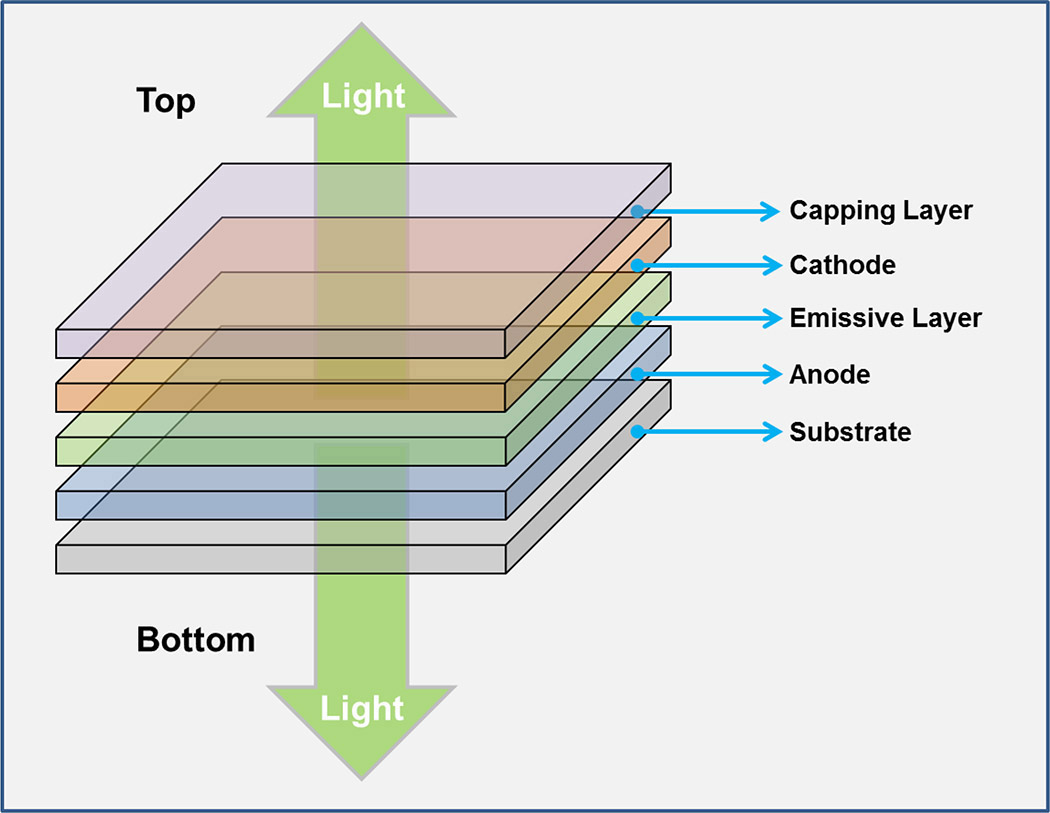
\includegraphics{figs/oled.jpg}
   \caption{Schematic diagram of OLED based on layered material showing how a functional device can be created from the combination of multiple layers that form an active region. At least one of the electrode layers in the device is made from a transparent conductor. Graphene is an ideal candidate material for transparent conducting electrodes in organic electronic devices. Reproduced with permission from:
\emph{SPIE Newsroom} November 2013: ``Transparent organic LEDs for new lighting applications,"  Jaehyun Moon, Jin Woo Huh, Chul Wong Joo, Jun-Han Han, Jonghee Lee, Hye Yong Chu and Jeong-Ik Lee.}

  \label{oled-fig}
\end{figure}

Application of organic materials in electronic technology offers many promising characteristics. First and foremost, many organic materials can be produced quickly and cheaply when compared to standard silicon semiconductor technology. Materials such as pentacene derivatives, perlyene derivatives like PTCDA, and carbon nanotubes are all carbon based materials which can act as semiconductors, which is the role silicon normally plays in a device. All of these materials can be synthesized with relative ease in a standard organic chemistry lab.

Many organic materials adopt structures that make them flexible while still retaining important electronic properties. Graphene and other sheet like polymer materials can be used as lightweight flexible conductors. Graphene in particular offers numerous other unique electronic properties making it an ideal candidate for study in organic electronics and will be the focus of later discussion. Flexibility in electronic devices is a property that is unknown to standard silicon based electronics. Mobile display technology, in the future, may make use of organic materials to create lightweight flexible OLED displays. A primary aim in integrating organic materials into electronic devices is to reduce cost. Transparent electrodes are necessary in many devices but current materials are often cost prohibitive; organic materials offer a low cost lightweight alternative.

Photovoltaic devices can be thought of, in principle, as an LED working in reverse. Thus it's easy to foresee that photovoltaic devices can be constructed using organic materials. Indeed organic photovoltaic (OPV) devices using fullerenes are in production for over two decades \cite{all-carbon}. In fact, it is possible to create an OPV device using only carbon \cite{all-carbon}. Carbon based materials in OPV devices offer the ability to create novel device architectures by making use of the flexible nature of organic materials. Flexible solar panels will allow greater adoption of solar power in modern society by greatly increasing the number of areas that can house photovoltaic devices. Lightweight flexible electronics and photovoltaics offer great possibilities for both terrestrial electronic applications as well as those used in satellites and space flight missions.

Finally, the environmental aspect of using organic materials in everyday electronic devices offers great promise. Organic electronic devices can be more energy efficient, which is beneficial, however, the benefit goes further. The manufacturing process used to create the devices promises to be more eco-friendly when compared to today's methods of electronic device production.

The benefits of organic electronic devices, their impact on our society, and a vision for the future have been laid out by the participants of the 2012 Chemical Sciences and Society Summit (CS3), briefly summarized here \cite{cs3}:
\begin{enumerate}
\item
Organic electronic devices will do things that silicon-based electronics cannot do.

\item
Organic electronic devices will be more energy-efficient and eco-friendly.

\item
Organic electronic devices will be manufactured in a more resource-friendly and sustainable fashion.
\end{enumerate}
All of the above statements indicate how organic electronics can be integral in contributing to a more sustainable future for our society.

\section{Graphene}
Graphene is an allotrope of solid carbon consisting of a single layer of $sp^2$ hybridized carbon atoms arranged in a hexagonal two-dimensional crystalline lattice. First isolated in 2004, graphene was the first truly two-dimensional material isolated in a lab setting \cite{apsnews}. Previously 2D materials were theorized to be thermally unstable and thus believed to not exist in nature \cite{Geim}. Thus, the isolation of graphene sparked an explosion of research. The entirely new field of study, 2D materials, seeks to analyze the properties of 2D materials and search for other materials, which are, like graphene, thermodynamically stable in a 2D crystalline phase. These materials present a rich variety of interesting properties making them useful in novel electronic architectures. To clarify the terminology, the designation of a material as two-dimensional stems from the fact that the mathematics describing the symmetry of the crystal lattice is purely two-dimensional. Many materials labeled as two-dimensional may contain multiple layers of atoms but the lattice as a whole has two-dimensional symmetry.

The honeycomb structure of graphene arises from the electron orbital hybridization in the carbon atoms. The $sp^2$ hybridization occurs when a carbon atom is bonded to three other atoms; in the case of graphene, all atoms are carbon. The bond hybridization results from a mixing between a carbon $2s$ orbital and two carbon $2p$ orbitals. This creates a set of three hybrid bonds where the state of minimal overlap between adjacent bonds manifests with a $120^\circ$ bond separation. This structure suggests crystalline graphene exists as a single sheet of carbon atoms where the nearest neighbor distance is 1.42 {\AA} with the actual hexagonal lattice constant larger by a factor of $\sqrt{3}$ at 2.46 {\AA}.  A diagram of the graphene structure can be seen in Figure \ref{Graphene-Structure-Figure}.

One of the interesting aspects of the graphene crystal structure is the two-atom unit cell. The hexagonal unit cell is made by adjoining only next-nearest neighbor carbon atoms, which are separated by a distance of 2.46 {\AA}. This means that nearest-neighbor carbon atoms are distinct from one another, these atoms are frequently labeled as A/B carbon atoms.  The lower portion of Figure \ref{Graphene-Structure-Figure} displays this characteristic. From this viewpoint, the graphene lattice can be considered as built from two separate interpenetrating trigonal lattices. The two-atom unit cell has direct implications for the electronic properties of graphene, which will be discussed later.

\begin{figure}
    \centering 
        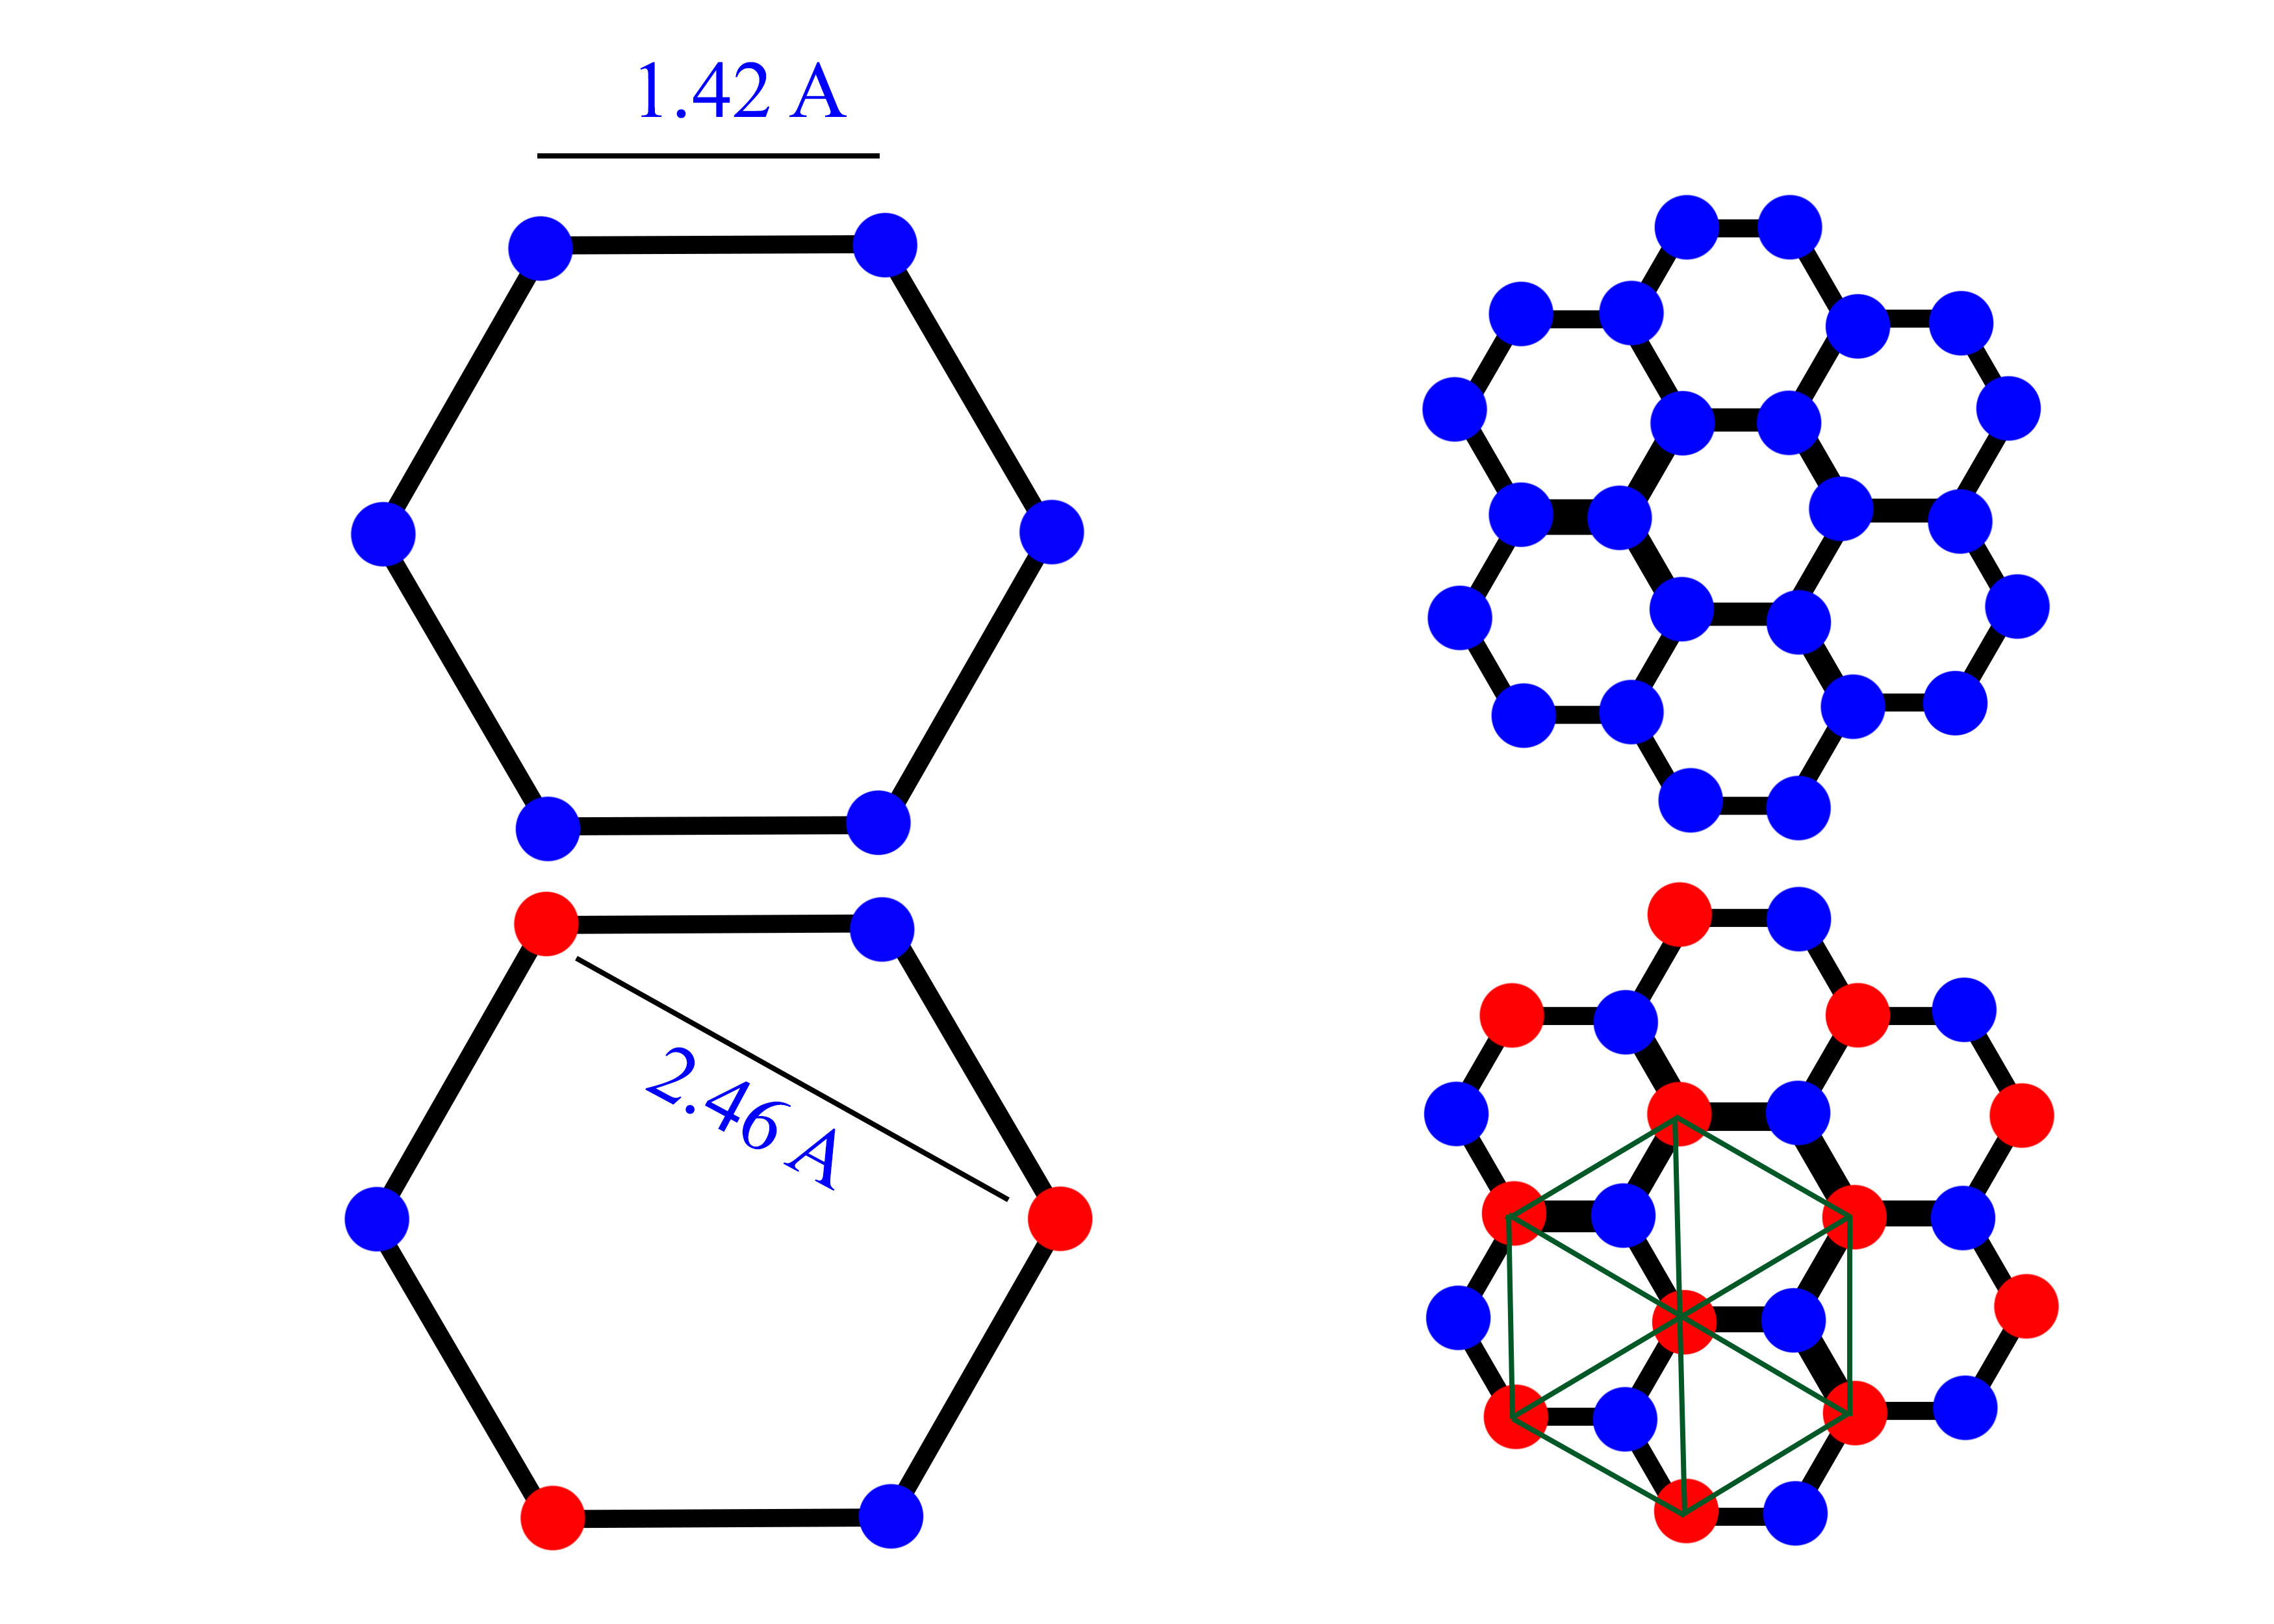
\includegraphics{figs/hexagonswithlength.jpg}
    \caption{Graphene honeycomb structure: (upper figure) 1.42 {\AA} nearest neighbor carbon distance. (lower figure) Characteristic two-atom unit cell: The nearest neighbor carbon atoms are distinct from each other and thus each graphene unit cell contains two atoms with lattice constant 2.46 {\AA}.
}
\label{Graphene-Structure-Figure}
\end{figure}

Soon after isolation, scientists studied and characterized numerous physical, optical, and electronic properties of the material. Graphene has a very high intrinsic electron mobility, in fact it has the highest mobility ever recorded \cite{Wolf}. A single sheet of graphene is nearly entirely transparent, only absorbing roughly 3\% of white light incident on the surface. This unique combination of high optical transparency with high electron mobility makes graphene an ideal candidate material for use as a transparent conductor in photovoltaic and light emitting devices such as OLED displays and flexible solar panels.

Currently, the material used in most devices in the role of a transparent conductor is indium tin oxide (ITO). Usage of ITO has a number of downsides. Namely, ITO is an expensive material to produce and apply in a device. The structure of ITO does not lend itself to flexibility without being incorporated into a polymer or nanofiber substrate, thus restricting device form factor. Finally, ITO, like many heavy metals, can cause health problems if inhaled or ingested which is a problem for recycling processes, and ITO also poses concerns for pollution in landfills.

Graphene has a wide variety of unique properties, many stemming directly from the 2D nature of the material. While graphene possesses a number of novel electronic properties, this doctoral work will focus primarily on the structural properties of graphene especially with regards to how the structure changes topology with respect different substrates. Finally the graphene surface structure will be analyzed from the viewpoint of a molecular scaffold for the self-assembly of atomic clusters and layers of organic semiconducting molecules.

\section{Self-Assembly}

It is often useful to think about nanoscale device fabrication from a top-down approach such as the familiar methods of etching devices into a silicon wafer via various lithographic techniques. However, another valid way to construct devices is to consider a bottom-up approach. Using this method, individual layers of materials are grown or deposited on a surface and combine to make an active region for a device in a layer-by-layer fashion. In order to improve device efficiency in a layered device, control over charge transport throughout and within the layers is of utmost importance.

When a material is grown or deposited onto a surface, the orientation of individual atoms or molecules within the material has a profound impact on the electronic properties of the material and thus on the device as a whole. The intermolecular forces combine with molecule-substrate forces to determine the overall topology of the layer. The strength of the intermolecular forces impacts the ability to transfer charge between molecules within a layer.

The growth process of a layer of molecules upon a crystalline surface is not guaranteed to produce a layer of material with any long-range intra-layer order. For example, consider analysis of the growth of derivatives of the prototypical organic semiconductor, pentacene, atop the gold (111) surface.  Scanning Tunneling Microscopy (STM) studies demonstrate with molecular resolution, that many phases of molecular packing relative to the gold surface coexist with poor long-range ordering \cite{wang-nano}. From a device standpoint, this inherent disorder within the pentacene layer is problematic. In the ideal scenario, all the pentacene molecules would adopt a single crystalline phase, thereby enhancing the ability to transfer charge between molecules within a layer.

There are a number of possible ways to address the issue of intra-layer order in a layered device. For example, many organic molecules provide a nearly endless amount of possible derivative molecules, which can be created or engineered by careful substitution of one atom or functional group for another. The addition of functional groups and substituent atoms to an organic molecule can have profound implications for not only the device characteristics but also the packing arrangement and preferred orientation of the molecule relative to the surface \cite{amanda-ttpo, bogdanc60}.

Outside of chemical functionalization, substrate modification provides another route towards guiding molecular orientation. Growth of pentacene derivatives on the stepped vicinal surface of gold (788) demonstrates the ability to create long-range intra-layer order within a monolayer of organic materials \cite{wang-nano}. The concept of surface structure modification as applied to growth of organic adsorbate layers and metallic clusters will be examined later with respect to the graphene surface.

The methods described above outline a process known as molecular self-assembly, the process through which molecules, atoms, or clusters of atoms or molecules adopt themselves into a well-defined arrangement without an external force to guide them into position. The ultimate goal of molecular self-assembly is to create new functional materials by assembling materials into an ordered supra-molecular device. Already many devices based on self-assembly have been created, such as bi-layer heterojunctions created from ordered organic semiconductors used in OLEDs and OPVs \cite{opv-self-assembly}. The latest advance in device design utilizing molecular self-assembly is the creation of a superconducting material by self-assembling a niobium-nitride in a matrix of organic block-copolymers. This marks the first superconducting device based on molecular self-assembly \cite{superconductor-self-assembly}.

Understanding molecular self-assembly requires an intuitive knowledge of the many forces that dictate molecular arrangement at the nanoscale. These forces can be strong forces such as those arising from the covalent bonding between adsorbate atoms and substrate atoms, however, often there are many very weak forces that much also be considered. Weak inter-molecular forces arising from dipole-dipole interactions, van der Waals interactions, and $\pi-\pi$ stacking are common in organic molecules and their contribution to molecular orientation cannot generally be overlooked. The presence of long-range weak forces also poses a problem for computational modeling of many organic molecules using density functional theory.

The UNH surface science lab has a rich history of preparation and analysis of a wide range of nanoscale molecular systems ranging from metallic nanoclusters to layered organic semiconductor heterojunctions. Previous work with fullerenes and pentacenes on gold and silver substrates has demonstrated the ability to engineer order within a molecular layer \cite{bogdan-sulfur, bogdanc60, wang, wang-nano, amanda-ttpo}. My doctoral work with graphene seeks to extend previous work with classic organic materials and metallic substrates and apply the same principles to a graphene system that possesses a novel surface structure.

\section{Surface Science}
The UNH surface science lab is uniquely equipped to probe the fundamental physics of the nanoscale world that takes place at the surface or interface between surfaces of a variety of novel materials. The primary reason surfaces are of interest is due to the fact that they represent a unique departure from the periodicity of three-dimensional materials. Surfaces represent a broken symmetry in one direction of an otherwise perfectly periodic solid material. This implies the atoms at the surface are distinct from atoms in the bulk material as they have a lower coordination number and thus often a higher chemical reactivity as well possibilities for localized quantum states not found in bulk.

Surface physics is crucial to understanding atomic reconstruction in solid crystals, epitaxial growth of layered materials, surface states and plasmons, as well as molecular self-assembly among many other topics. Knowledge of surface and interface physics is important for understanding many physical and chemical processes such as catalysis, photovoltaic energy production, oxidation and, corrosion. The study of catalysis is likely the original motivation for research in surface science however the driving factor in the modern explosion of surface science research is fabrication of semiconductor devices \cite{SurfSciTechniques}. The characterization of semiconductor surfaces, in general, requires detailed knowledge of atomic reconstruction relative to the bulk structure. Examples of this can be seen in the complex surface reconstructions of silicon and silicon carbide. Thus to adequately understand physics at the surface, tools for discerning precise atomic positions are needed \cite{SurfSciTechniques}.

In order to study surfaces at a fundamental level, a pristine environment is required to preserve the atomic composition over significant time scales. Thus much work in surface science and all work in this thesis takes place in an ultra high vacuum (UHV) environment. In UHV, a surface prepared for an experiment can be considered clean or well characterized for many hours before any significant contamination has built up. This leaves ample time for surface sensitive experiments to take place.

The primary work this thesis utilizes for surface analysis is scanning tunneling microscopy (STM). STM is a non-optical form of microscopy using a scanning metallic probe and quantum tunneling to extract data and generate images of the local density of electronic states at the surface. Quantum tunneling has no classical analog and is a physical phenomenon restricted solely to the nanoscale regime.

STM is a powerful tool for probing the real space structure of surfaces with unmatched resolution in all directions. While the data directly produced by an STM is a map of the local density of states in the surface, from this data the exact positions of atoms in the material can be extracted. Thus STM provides a way to map the topography of the surface with atomic resolution, something impossible with optical microscopy due to the diffraction limit of visible light. The ultra-high resolution provided by STM is extremely important for the study of molecular self-assembly and atomic reconstructions. The microscope used for much of my thesis work is a homebuilt variable temperature scanning tunneling microscope (VT-STM) housed in an ultra high vacuum chamber with an ultimate pressure better than $10^{-10}$ torr integrated with a number of other tools for surface preparation and analysis.

The second primary tool for surface analysis and preparation used in this thesis work is Low Energy Electron Diffraction (LEED). Whereas STM provides real space information about the surface with highly localized resolution, LEED provides momentum space information about the surface in a much larger sample area. Using LEED, the crystal structure of the surface region in a sample can be determined with relative ease. A related technique using the same LEED optics, Auger Electron Spectroscopy (AES) maps the surface elemental composition with a high degree of accuracy. LEED and AES together combine to make ideal tools for assessing and monitoring UHV sample preparation. The UHV system at UNH used for this thesis work is equipped with an Omicron SpectaLEED rear view LEED/AES system.

The reciprocal space images generated by LEED give qualitative information on how well ordered the sample surface is from a crystallographic standpoint. A well ordered single crystal surface has sharp precise diffraction maxima in reciprocal space whereas a sample with multiple domains or rotational disorder has diffuse diffraction maxima spread over a larger region in reciprocal space. The LEED pattern seen from a given surface represents a scaled version of the sample surface reciprocal lattice and contains information about rotational symmetries in the surface.

One of the major restrictions for conventional LEED systems is the beam geometry with respect to the sample blocking view of the spectrally reflected beam. At very low energies, all higher order beams exist at diffraction angles too large to be imaged. Since the spectral beam is blocked by the electron source, conventional LEED has a minimum energy in the 40-60 eV range where no data can be collected for incident beam energies lower than this threshold.

Of interest to the study of this novel graphene system are the interactions between very low energy electrons and layered surfaces and thin films. Very low energy electrons, E $<$ 20 eV, have unique interactions with thin films due to quantum confinement effects. These effects manifest as oscillations in the electron reflectivity curves. It has been shown previously that these oscillations can be used to map the layer thickness in thin films such as metallic monolayers or graphene layers \cite{Hannon-LEEM-Book}. To bypass the minimum energy restriction of conventional LEED systems, I utilize a third surface science technique called low energy electron microscopy (LEEM).

LEEM instruments are a subset of cathode lens microscopes, where the sample being probed is held at high negative potential and acts as part of the lens system itself. LEEM systems allow many different beam line geometries compared to conventional LEED through the use of magnetic prism arrays. This allows all reflected beams to be imaged simultaneously and also allows for imaging of the surface while a dynamic process such as epitaxial growth takes place. LEEM can also easily collect data at very low incident electron energy, thus the restriction of minimum energy from conventional LEED is lifted.

What separates LEEM primarily from LEED, however, are not just alternate geometries and energy ranges. Rather, LEEM can operate in both real space imaging mode and reciprocal space imaging mode and can switch between the two quite rapidly simply by swapping which optical plane is projected into the detection column. Thus a surface can be imaged with resolution on the order of a few nanometers in real space and without much effort, the same area of the sample can then be probed in reciprocal space using LEED techniques. Furthermore, the size of the area probed using LEED mode can be restricted well below that possible in conventional LEED setups. A LEEM instrument  allows LEED data to be collected from a selected area in the real space image using special contrast apertures added to the beam line. The combined ability to acquire high resolution real space surface images with localized reciprocal space data makes LEEM an incredibly powerful tool for surface sensitive studies.   

Finally, both LEEM and LEED experiments can provide three-dimensional information regarding the crystal structure near the surface region of the sample. While analysis of static LEED patterns provides information in the two-dimensional surface plane, additional three-dimensional information can be accessed using a technique called LEED/LEEM-I(V). By varying the energy of the incident electron beam and recording the intensity of the reflected or diffracted electrons, one can analyze how the electron reflectivity depends on energy. The shape of these electron reflectivity curves provides information about the three-dimensional atomic structure of the surface. This technique, however, requires close collaboration with theoretical modeling of the surface in order to fit the experimental curves to those predicted by theory.

To aid in the analysis of LEED and LEEM-I(V) data sets, I have designed a software package using python to visualize LEED and LEEM data and allow quick and reproducible extraction of I(V) curves. This software is currently being used to help with I(V) studies of numerous two-dimensional materials through collaboration external research groups. Analysis of LEEM-I(V) data from our graphene system will provide additional information about the system not easily achievable with STM or conventional LEED alone.

\section{Summary}
This thesis outlines research into a variety of novel materials for future application in electronic devices based on layered 2D materials. 
	My work focuses on the structural properties of a novel polymorphic graphene system, developed at UNH, which presents a unique structure that can be utilized as a template for molecular self-assembly. Control over the growth of clusters of metals and organic semiconducting molecules will be important to future work in enhancing efficiency in nanoscale electronic devices. Understanding the underlying physics, which governs charge transfer both within as well as between material layers in a nanoscale device, will be crucial to characterization of device parameters. Specifically, for organic electronic devices, it is important to understand how device structure and morphology affects processes such as diffusive charge transport, exciton recombination, and charge collection at electrodes.
	The materials discussed in this work have potential for use in a wide array of electronic devices from photovoltaic applications to organic electronic lighting and from highly sensitive chemical sensors to touch screen displays. Terrestrial applications of organic electronics are not the only market standing to benefit from advances in the field. Organic electronics and organic photovoltaics are also of great interest for satellite design and space flight missions to reduce cost, enhance power generation, and increase the overall efficiency of devices onboard.

\begin{itemize}
\item Chapter 1, \emph{Introduction} 
\item Chapter 2, \emph{Graphene}
\item Chapter 3, \emph{Tools for Surface Science}
\item Chapter 4, \emph{Polymorphic Graphene: modulating the graphene surface structure}
\item Chapter 5, \emph{LEEM/LEED-I(V) study of two-dimensional materials}
\item Chapter 6 \emph{Conclusions}
\end{itemize}

% ------------------- %
\chapter{\sc Graphene}
\label{ch:Graphene}

\section{Carbon and its Allotropes}

Carbon is possibly the most ubiquitous atomic element known to man. The fourth most abundant element in the entire universe behind only hydrogen, helium, and oxygen, carbon is found essentially everywhere one looks for it in one form or another. Originating from stellar nucleosynthesis, carbon is an important element in the evolution of different chemical elements in the history of the universe \cite{katsnelson}. As a result of its abundance, carbon plays a special role in human history with frequent and diverse usage in everything from metallurgy to medicine, and art to energy.

\begin{equation}
  \label{eq:photosynthesis}
  \ce{6 CO2(g) + 6 H2O(l) ->[ \gamma ] C6H12O6(s) + 6 O2(g)}
\end{equation}

Carbon has atomic number six and a valence number of four corresponding to an electron configuration of  $1s^2 2s^2 2p^2$. The tetravalent aspect makes carbon unique due the vast number of bonding schemes allowed by this electron configuration. The large number of bond formations allows an endless variety of molecules and allotropes based on carbon to form readily. Simple gases such as \ce{CO_2} and \ce{CH_4} are common to everyday life, however, more complex molecules like glucose, \ce{C_{6}H_{12}O_6}, are crucial to all life as we know it at the cellular level both in the Krebs cycle and also in photosynthesis. In fact, carbon is denoted the \emph{material prima}, or fundamental substance, for all life \cite{geim-elec}. The importance of carbon to the photosynthetic cycle is shown in equation \ref{eq:photosynthesis}. The complex sugars and hydrocarbon chains represent of the wide array of organic compounds possible through carbon chemistry, however, there are many forms of molecules and materials that can be made purely from carbon and no other elements.

The word allotrope refers to distinct physical forms of material made from a single element; carbon has numerous stable allotropes. The wide variety of carbon allotropes expose the rich geometry afforded to different bonding schemes from simple rings and linear chains to complex three-dimensional structures. Carbon is the only element thus far found to be stable in materials ranging from zero to three dimensions. This has profound implications on the material properties carbon can adopt, as a material's dimensionality is one of its most defining properties \cite{novoselov-2d}. Fullerene molecules made of nearly spherical cages of carbon rings demonstrate carbon in zero-dimensional form, though they are sometimes referred to as quasi-zero-dimensional. Carbon nanotubes are the manifestation of carbon in one-dimensional objects, and can be viewed as the linear extension of a buckyball in one direction. Graphene, a planar carbon structure, extends carbon to two-dimensional materials, and has the same structure as an unzipped or unrolled carbon nanotube. Finally graphite and diamond represent two separate ways of carbon bonding in three dimensions. These variants of solid carbon all have distinctly different physiochemical properties.

Graphite, named after the Greek \emph{graphos}, meaning to write, consists of many layers of $sp^2$ bonded carbon; each layer can be considered an individual graphene sheet \cite{history-thermodynamics}. These layers are only weakly bonded to each other in the direction perpendicular to the basal plane through van der Waals forces. This bond configuration is very weak relative to the covalent in-plane bonds and as a result the inter-layer coupling in graphite is also weak which allows the layers to slide against one another with relative ease. As a result, graphite is an ideal material for use in pencils or other marking devices and as a lubricant.

The primary material of interest in this thesis is the individual graphite layers known as graphene. The two-dimensional nature of this material directly bestows many interesting physiochemical properties. As the first direct evidence that two-dimensional materials can be thermodynamically stable, the discovery of graphene has spawned an entire new field of material science and physical research.

\section{Carbon in Two Dimensions: Graphene}
  \subsection{Discovery and History}
Discovery and usage of graphite dates back over 500 years \cite{honeycombcarbon}. The original uses for graphite were for writing, marking, and art, however, in the present graphite sees use as an industrial lubricant as well as the primary moderator in nuclear fission reactors. The structure and properties of graphene have been studied from a theoretical standpoint since the early work by Wallace in 1947 \cite{wallace}. This early work laid the foundation of considering graphite as a collection of weakly interacting carbon layers. In this sense, each carbon layer can be effectively considered independent from the others and thus the electronic structure can be modeled by considering only one layer. At the time, however, it was widely believed that a single layer by itself would be thermodynamically unstable \cite{Geim}.

	The study of epitaxial growth of carbon layers on various metal surfaces dates back to the 1970's. Measurements of the properties of the carbon layers were, however, always skewed by the strong interaction between carbon and metals. This made measuring pure graphene-like properties difficult. In the early 2000's work continued on isolating single or few carbon layers from graphite. Graphite is commonly used in STM laboratories as an ideal sample for calibration of the microscope due to the periodic surface structure and ease of sample preparation. A common method to prepare the surface of graphite is simply to apply adhesive tape to the surface and peel away the tape. This adhesion between surface carbon layers and the tape is much stronger than the layer-layer bonding in the graphite. Thus, carbon layers can easily be peeled away from a bulk graphite crystal.

	The breakthrough in isolating single layer graphene came from Andre Geim and Kostya Novoselov at the University of Manchester in 2004. Careful analysis of the carbon remnants on adhesive tape from cleaved graphite lead to the discovery that some exfoliated carbon layers were thicker than others. Continued work lead to the isolation of single layer carbon after an important discovery that graphene would be optically visible when placed on a silicon dioxide substrate with carefully chosen thickness \cite{Geim}. Confirmation of single layer graphene demonstrated for the first time that a material could be stable as a single atomic layer. This work, which lead to a Nobel prize for Geim and Novoselov in 2010, spawned an explosion in fundamental research of the properties of two-dimensional materials.

  \subsection{Structure}
 Graphene consists solely of $sp^2$ hybridized carbon atoms. This bond configuration is found in single graphene sheets, in three-dimensional graphite, as well as in other organic molecules such as benzene. The structural bonds connecting nearest neighbor carbon atoms are called $\sigma$ bonds. In the $sp^2$ configuration each carbon atom is bonded covalently to three other carbon atoms with an average bond distance of 1.42 {\AA}. Mathematically the $\sigma$ bond in graphene is a linear combination of the $2s$ and $2p$ electron orbitals. In order to minimize the overlap between individual $\sigma$ bonds, the bonds are separated by an angle of $120^{\circ}$. All three bonds lie within a single two-dimensional plane and thus accordingly, graphene is deemed a two-dimensional material.

 \begin{figure}
    \centering
         \includegraphics[scale=0.65]{figs/graphene-unit-cell.png}
    \caption{
Graphene honeycomb lattice shown composed of alternating A (red) and B (blue) carbon atoms. The graphene unit cell is highlighted in grey showing that the cell contains two distinct carbon atoms.
}
    \label{fig:graphene}
\end{figure}


 \begin{figure}
     \centering
         \includegraphics[scale=0.55]{figs/graphene-reciprocal-lattice.png}
     \caption{ The graphene real space hexagonal lattice is accompanied by a hexagonal reciprocal space lattice. Shown here is the reciprocal unit cell relative to the first Brillouin zone; the important high symmetry points are labeled, notably the K and K' points are distinct from one another.
}
     \label{fig:graphene-reciprocal}
\end{figure}

 Carbon is tetravalent, thus, outside of the structural bond configuration, which occupies three of the four valence electrons, each carbon atom in the graphene structure has one free electron. Again to minimize the overlap with the structural bonding $\sigma$ orbitals, the free electron fills the remaining $n=2$ electron orbital. Conventionally the electron orbitals that hybridize to create the $\sigma$ bonds are labeled as the spherically symmetric $2s$ orbital as well as the $2p_x$ and $2p_y$ planar orbitals. The graphene structure then lies solely in the x-y Cartesian plane. The sole unfilled $n=2$ orbital is then the $2p_z$ orbital, which lies perpendicular to the structural bonding plane. For each carbon atom, one electron fills the $2p_z$ orbital and is not responsible for in-plane structure. The nearest neighbor carbon distance is large enough that there is very weak overlap between the $2p_z$ orbitals. However, there is still a non-zero overlap between neighboring $2p_z$ orbitals, this electron orbital overlap is called a $\pi$ bond.

 The out of plane $\pi$ bonds in an individual graphene sheet are responsible for the three dimensional structure of graphite when multiple layers are stacked atop one another. The $\pi-\pi$ stacking between layers is very weak relative to the intra-planar $\sigma$ bonding. This weak bonding allows individual graphene planes to slide parallel to the basal plane relative to other carbon layers with ease. Considering just a single graphene layer, the pi bonds are delocalized from the planar structure, and thus the electrons in these orbitals are responsible for the unique electronic properties of graphene, which will be explored later.

 Since the structural bonding in graphene lies within a two-dimensional plane, graphene is labeled as a two-dimensional material. Currently graphene is the thinnest material in existence that is thermodynamically stable at ambient conditions and has been prepared in a lab setting. While there are other single element two-dimensional materials, given the general trend for average atomic radii there are few options for materials that would be thinner than graphene. In fact, many other group IV elements such as silicon, germanium and tin have been theorized to have two-dimensional allotropes. They are named in similar fashion to graphene, namely silicene (Si), germanene (Ge), and stanene (Sn). While the carbon atoms in graphene remain coplanar, the hexagonal arrangement of atoms in other group IV two-dimensional materials generally adopts a buckled bilayer structure.

Here it is worth noting that while the theoretical structure of freestanding graphene should be atomically flat up to micrometer scales, there are currently no methods of producing large scale freestanding graphene, thus in practice the structure of the carbon layer will be dependent on the substrate on which it lies. Graphene can be grown atop a wide variety of crystalline and amorphous substrates from simple metals such as nickel and copper to more complex semiconductor surfaces such as silicon carbide. The structure of the carbon layer can change drastically as a result of the topology of the underlying substrate surface structure and thus as a result the properties of the graphene layer may depart from those of ideal freestanding graphene.

  \subsection{Significance: Paradigm shift to 2D}

 While it has already been mentioned that the discovery of graphene essentially launched the field of two-dimensional materials into notoriety, the significance warrants further discussion. After the isolation of graphene, numerous other layered van der Waals materials were examined as candidates for two-dimensional isolation. Quite quickly it was found that materials such as hexagonal boron nitride, molybdenum disulfide, and niobium diselenide could be treated in a similar manner to graphite to produce two-dimensional materials \cite{novoselov-2d}. The later materials fall into a category of materials called transition metal dichalcogenides, TMDs. It is now known that this family of materials hosts a plethora of materials suited for two-dimensional applications. These further studies demonstrate that graphene is not the anomaly in the nouveau two-dimensional material world; rather there exists a potentially endless realm of new materials with distinct and exciting properties.

  The discovery of materials that can be isolated in two-dimensional form, while noteworthy as it was originally theorized to be impossible, only provides the scaffolding for the search for new physics in two-dimensions. The study of material properties in the two-dimensional limit truly garners excitement in the world of material science. The vast assortment of two-dimensional materials fully spans the configuration space of material properties. While graphene possesses unique electronic properties as a zero-gap semiconductor, some TMDs display interesting changes in their band structure as their thickness decreases to the two-dimensional limit. For example, bulk molybdenum disulfide, \ce{MoS_2}, is an indirect gap semiconductor with a band gap of approximately $1.23$ eV. When the bulk crystal is exfoliated to produce two-dimensional monolayer samples, the electronic properties change drastically and the material manifests as a direct gap semiconductor with a band gap of roughly $1.8$ eV \cite{monolayer-mos2, 2d-atlas}. While many TMDs are characterized as semiconducting materials, other 2D materials exhibit more exotic electronic properties such as superconductivity and charge density waves \cite{2D-TMDs}.

  That many two-dimensional materials are stable in ambient conditions while also retaining their unique properties is of great significance. The variety of electronic properties found in two-dimensional materials makes them ideal for applications in new ultra-thin flexible electronic devices. The optical properties found in two-dimensional materials open new avenues for photovoltaic devices as well as photosensors for light spectra difficult to absorb with conventional silicon technology \cite{ graphene-2d-optoelectronics}. Furthermore, there are many novel electronic devices, such as tunnel-junction transistors, which are only functional when constructed with ultra-thin heterojunctions. Two-dimensional semiconductors provide a new avenue for exploration of these devices. Many interesting properties of two-dimensional materials stem directly from the unique surface structure adopted by the materials; the link between graphene's structure and its sought after characteristics will be explored further.

\section{Properties and Applications}
  \subsection{Structure Review}
Graphene forms a two-dimensional honeycomb lattice with a nearest neighbor separation of 1.42 {\AA} and a lattice constant of 2.46 {\AA}. The graphene unit cell contains two distinct carbon atoms, thus the graphene lattice can be considered two interpenetrating trigonal sublattices. These sublattices are commonly referred to as A and B as shown in figure \ref{fig:graphene}. This lattice geometry, where A atoms are bonded to only B atoms and vice versa is known as a bipartite lattice \cite{katsnelson}. Profound consequences arise from the fact that nearest neighbor atoms in graphene are distinct from one another. This was first recognized in the treatment of the graphite band structure by Wallace in 1947 \cite{wallace}.

The graphene reciprocal lattice also displays the symmetry of the real space two atom unit cell. A hexagonal lattice in real space is accompanied by a hexagonal reciprocal space lattice. The fact that graphene has two distinct atoms in its real space unit cell means that certain high symmetry points in the first Brillouin zone will be distinct from one another. As shown in figure \ref{fig:graphene-reciprocal} the K and K' points are distinct in reciprocal space. These special high symmetry points in reciprocal space, K and K', are called the Dirac points. Equation \ref{eq:k-points} gives the cartesian coordinates of K and K' in terms of the graphene nearest-neighbor distance $a =  1.42${\AA}.

\begin{align}
\label{eq:k-points}
\begin{split}
\vec{K}^{\, '} = ( \frac{2\pi}{3a}, \frac{2\pi}{3 \sqrt{3} a} ) \\   \vec{K} = ( \frac{2\pi}{3a}, \frac{-2\pi}{3 \sqrt{3} a} )
\end{split}
\end{align}

The structure of graphene and the underlying symmetry of its crystalline lattice play an important role in governing the many unique physiochemical properties manifested in this two-dimensional material. The structural bonding consisting of the graphene $\sigma$ bands are a filled valence shell, whereas the $\pi$ bands contain only one electron per atom and are thus only half filled. The existence of half filled bands is important to the underlying physics and electronic properties; half filled bands suggest metallic behavior, however, we will see later that graphene does not display perfectly metallic nor standard semiconducting behavior \cite{geim-elec, kitel}. The wavefunction describing an electron in the $\pi$ band of graphene must have a quantum number distinguishing which sublattice the electron originates from due to the two atom nature of the graphene unit cell. This give only two choices, namely A or B. The two level system can be mathematically represented as an isospin or pseudo spin degree of freedom for the graphene wavefunction as a direct result of the symmetry of the lattice structure \cite{Wolf}.

  \subsection{Electronic Structure}
  	The band structure of the graphene $\pi$ bands was first studied in detail by Wallace in 1947 and furthered by McClure in 1957 \cite{wallace, mcclure}. These early attempts focused on graphite, as graphene was not yet known to exist in a stable form. Due to the weakly interacting nature of the individual layers in graphite, the derived band structure correctly predicts that of graphene.

	As previously mentioned, the properties of graphene are generally highly dependent on the substrate on which it is grown. In order to approximate freestanding graphene, one can engineer a substrate with holes and suspend a graphene layer across the gap. Here we will introduce a model of the electronic properties of free standing graphene and then later discuss how substrates may affect the observed properties.

	Each carbon atom in the graphene lattice contains one free electron in a $\pi$ state, and only these electrons contribute to conduction. Thus, for simplicity, only the band structure of the $\pi$ band will be considered. The simplest model of graphene uses a tight-binding approximation considering only interactions between electrons in nearest-neighbor atoms. Given the bipartite graphene lattice, two $\pi$ states represent the basis for the Hamiltonian of the system. Considering only nearest-neighbor interactions then suggests that only interactions between electrons from differing sublattices will contribute to the Hamiltonian. This results in a simple $2x2$ matrix describing interaction between the A and B electron states.

	Consideration of only interactions between different sublatticies implies that only the off diagonal elements contribute to the total Hamiltonian. These elements can be characterized with two features. First there must be a parameter to represent the strength of the interaction. This is known as the hopping parameter and denoted by t, which is a constant with units of energy. Finally the off diagonal terms represent the overlap between an electron on sublattice A with an electron on sublattice B. The overlap of these two wavefunctions is a function of the electron wave vector, $\vec{k}$, and is denoted by $S(\vec{k})$. Equation \ref{eq:ham-mat} shows the matrix representation of the tightbinding Hamiltonian as a function of electron wave vector, $\vec{k}$ \cite{katsnelson}.

	The tight binding Hamiltonian can also be represented easily using the concept of creation and annihilation operators for electrons on the A and B sublattices, $\{\hat{a}, \hat{a}^{\dagger}, \hat{b}, \hat{b}^{\dagger} \}$, as shown in equation \ref{eq:ham-eq}. In this formulation, the sum extends over all lattice sites, denoted by $i$ and $j$, connected by a nearest neighbor distance of 1.42 {\AA}. In principle the sum extends over all spin degrees of freedom as well but this is excluded for simplicity. The operator notation is as follows: $\hat{a}_{i}^{\dagger}$ creates an electron on the A sublattice at lattice site $i$, $\hat{b}_{j}$ annihilates an electron from the B sublattice at lattice site $j$. The parameter, $t$, is again the nearest neighbor hopping energy, a constant roughly equal to $2.8$ eV \cite{geim-elec}.

\begin{equation}
\label{eq:ham-mat}
\hat{H}(\vec{k}) = \begin{pmatrix}
0& tS(\vec{k})\\
tS^*(\vec{k})& 0
\end{pmatrix}
\end{equation}


\begin{equation}
\label{eq:ham-eq}
\hat{H}(\vec{k}) = -t \sum_{<i,j>}( \hat{a}_{i}^{\dagger} \hat{b}_{j} + \hat{b}_{j}^{\dagger} \hat{a}_{i} )
\end{equation}


Following Katsnelson, the overlap functions, $S(\vec{k})$, can be written as a sum over all nearest neighbor vectors as shown in equation \ref{eq:overlap} \cite{katsnelson}. Here $\vec{\delta} \epsilon \{ \vec{\delta_1}, \vec{\delta_2}, \vec{\delta_3} \}$, where $\vec{\delta_i}$ represents one of three real space nearest neighbor vectors in the graphene unit cell. The right hand side of equation \ref{eq:overlap} comes from an analysis of the coordinates of the graphene unit cell relative to that shown in figures \ref{fig:graphene} and \ref{fig:graphene-reciprocal}.
 \begin{equation}
 \label{eq:overlap}
 S(\vec{k}) = \sum_{\vec{\delta}} e^{i \vec{k} \cdot \vec{\delta} } = 2 e^{\frac{i k_x a}{2}} \cos{( \frac{k_y a \sqrt{3}}{2})} + e^{- i k_x a}
 \end{equation}

The energy of an electron, $E(\vec{k})$ can be calculated from the Hamiltonian given in equation \ref{eq:ham-mat} as shown in equations \ref{eq:energy} and \ref{eq:overlap-proof}. Here the + refers to the upper ($\pi^{*}$) band and the - refers to the lower $\pi$ band. Note that this simple model predicts precisely $E = 0$ for $\vec{k} = \vec{K}$ or  $\vec{K^{'}}$. This suggests that the bands cross at the Dirac points and the energy at the Dirac points is exactly zero. One of the fundamental characteristics of graphene's electronic structure is the exactly zero energy gap at the Dirac points. This classifies graphene as a zero band gap semiconductor.

The area in k-space in the vicinity of the Dirac points displays a unique dispersion relation with numerous interesting implications. Dispersion near $\vec{K}$ and $\vec{K'}$ is linear to first order; this is quite a staunch departure from the typical quadratic relation between electron energy and momentum in solid materials $E(\vec{k}) = \frac{k^2}{2m}$.
 \begin{equation}
 \label{eq:energy}
 E(\vec{k}) = \pm t|S(\vec{k})| = \pm t \sqrt{S(\vec{k}) S^{*}(\vec{k})} = \pm t \sqrt{3 + f(\vec{k})}
 \end{equation}
 \begin{align}
 \label{eq:overlap-proof}
 \begin{split}
 S(\vec{k}) S^{*}(\vec{k}) & = (2 e^{\frac{i k_x a}{2}} \cos{( \frac{k_y a \sqrt{3}}{2})} + e^{- i k_x a})(2 e^{\frac{-i k_x a}{2}} \cos{( \frac{k_y a \sqrt{3}}{2})} + e^{i k_x a}) \\
 & = 1 + 4\cos^2{(\frac{k_y a \sqrt{3}}{2})} + 2e^{\frac{3 i k_x a}{2}}\cos{(\frac{k_y a \sqrt(3)}{2})} + 2e^{\frac{ - 3 i k_x a}{2}}\cos{(\frac{k_y a \sqrt(3)}{2})}\\
 & = 1 + 4\cos^2{(\frac{k_y a \sqrt{3}}{2})}  + 4\cos{(\frac{3 k_x a}{2})}\cos{(\frac{\sqrt{3} k_y a}{2})}\\
 & = 1 + 4(\frac{1}{2}(\cos{(\sqrt{3} k_y a)} +1)) + 4\cos{(\frac{3 k_x a}{2})}\cos{(\frac{\sqrt{3} k_y a}{2})}\\
 & = 3 + 2\cos{(\sqrt{3} k_y a)} + 4\cos{(\frac{3 k_x a}{2})}\cos{(\frac{\sqrt{3} k_y a}{2})} \\
 & = 3 + 	f(\vec{k})
 \end{split}
 \end{align}

 While the Hamiltonian given in equations \ref{eq:ham-mat} and \ref{eq:ham-eq} correctly predicts the zero band gap nature of graphene and  linear dispersion near the Dirac points, a more accurate description can be developed by including next nearest neighbor interactions. This requires the addition of another parameter, $t^{'}$, to characterize the hopping energy for next nearest neighbor exchange. Equation \ref{eq:ham-eq2} shows the form of the Hamiltonian built from creation and annihilation operators including next nearest neighbor interaction. The dispersion relation derived from this Hamiltonian, $E(\vec{k})$, is shown in figure \ref{fig:dispersion} where an additional parameter for next-nearest neighbor interactions has been included, $E(\vec{k}) = \pm t \sqrt{3 + f(\vec{k})} + t^{'}f(\vec{k})$ \cite{geim-elec}. It is interesting to note that the inclusion of next nearest neighbor interactions preserves the dispersion relation near the Dirac points as well as the zero energy gap, however, the energy at the Dirac points is no longer zero, $E(\vec{k}=\vec{K}) = -3t^{'}$ \cite{geim-elec}.

 \begin{figure}
 \centering
         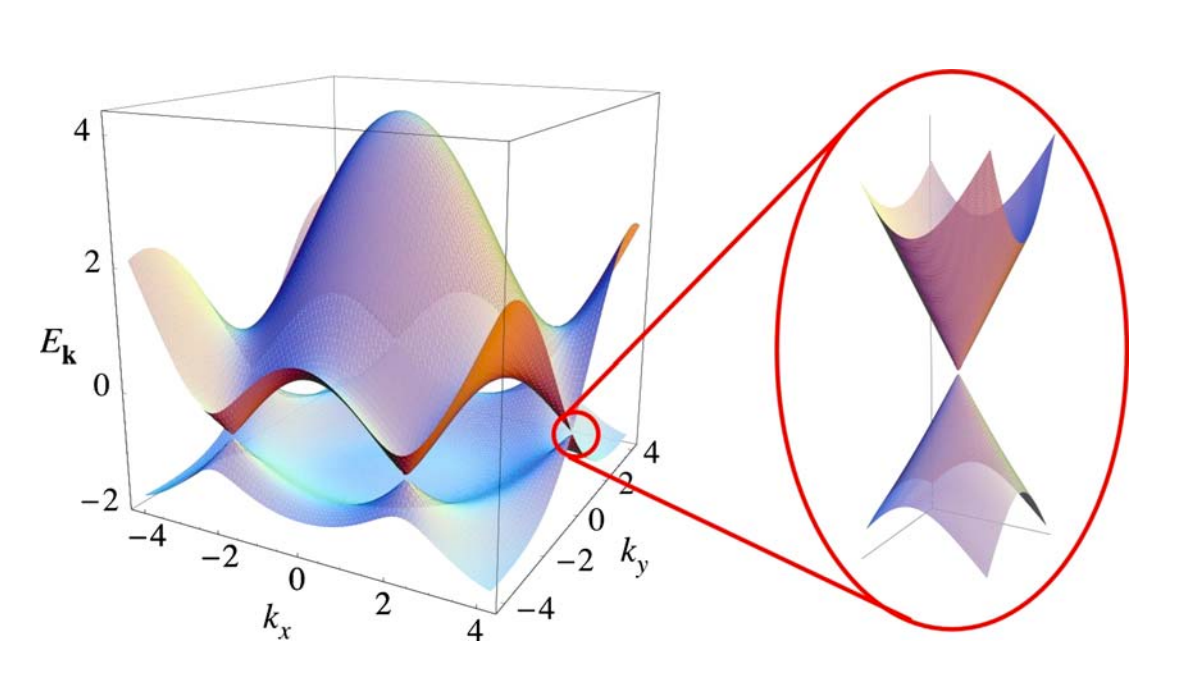
\includegraphics[scale=0.40]{figs/Graphene-Dispersion.png}
    \caption{Left: Energy bands for graphene with nearest neighbor and next-nearest neighbor hopping parameters set to $t=2.8 eV$ and $t^{'}=-0.2t$. Right: Expanded view of electron dispersion near the Dirac point displaying characteristic linear dispersion. Reproduced with permission from American Physical Society Copyright (2009) \cite{geim-elec}.
    }
    \label{fig:dispersion}
\end{figure}

\begin{equation}
\label{eq:ham-eq2}
\hat{H}(\vec{k}) = -t \sum_{<i,j>}( \hat{a}_{i}^{\dagger} \hat{b}_{j} + \hat{b}_{j}^{\dagger} \hat{a}_{i} )  -t^{'}\sum_{<<i,j>>}(\hat{a}_{i}^{\dagger} \hat{a}_{j} + \hat{a}_{j}^{\dagger} \hat{a}_{i} + \hat{b}_{i}^{\dagger} \hat{b}_{j} + \hat{b}_{j}^{\dagger} \hat{b}_{i} )
\end{equation}

The physics of charge carriers near the Dirac points in graphene exhibits numerous interesting characteristics that distinguish graphene from other materials. The dispersion near the Dirac point mimics that of massless Dirac fermions, where the charge carriers move at a fixed speed, $v_f  = \frac{3ta}{2\hbar}\approx \frac{c}{300}$, where $c$ is the speed of light in vacuum. Here the massless aspect can be seen by first considering the energy formula dictated by special relativity, $ E = [(pc)^2 + (mc^2)^2]^\frac{1}{2}$.  Here p is the particle momentum, c the speed of light in vacuum, and m is the mass of the particle. Thus in the limit where m goes to zero, the form of energy recovered is $E = pc = v_f \hbar | \vec{k}-\vec{K}|$ \cite{Wolf}. Thus for k near the Dirac points, the energy dispersion in graphene is linear with respect to momentum, as would be expected for a massless particle with relativistic velocity.



  \subsection{Optics}
  One of the most direct applications of graphene concerns its use as a transparent electrode material in photovoltaic and optical applications. Graphene is ideal for this application due to its lightweight and flexibility, but most of all as a result of its high degree of transparency. With an adsorption of only 2-3\% of white light, graphene is nearly totally transparent and yet at the same time offers a high conductivity \cite{graphene-optics}. These two properties together are highly sought after in photovoltaic electrode materials.

The most common material in use for transparent electrodes is currently Indium Tin Oxide, ITO. In principle, graphene offers a cheaper and more environmentally friendly material while also providing an opportunity for flexibility. Graphene's optical transmittance as a function of wavelength is highly superior to that of ITO as the transmittance of ITO drops off heavily in the UV range \cite{ graphene-synth-app, graphene-opto}.

However, in practice the cost to manufacture a graphene based photovoltaic cell will be largely dependent on advances in production for graphene. Also, plain graphene electrodes suffer from issues with high contact resistance, which can dramatically reduce the efficiency of the photovoltaic cell.

 \subsection{Use in organic electronics}

 One of the most notable applications of graphene falls in the field of organic electronics. Graphene is an ideal material for use in organic photovoltaic technology as a transparent electrode. The inherent flexibility of the material opens avenues for flexible organic photovoltaics as well as flexible organic LEDs. Flexibility in photovoltaic technology can allow for the adoption of solar power generation in many areas where it is currently prohibited due to device form factor such as clothing and portable electronics. Finally, given the prevalence of smart devices with touch screen technology, graphene again is an ideal candidate for integration as a transparent electrode with the ability to conform to novel geometries while retaining ideal electronic properties \cite{Wolf-apps}.

 \subsection{2D Materials and Nanoelectronics}
 As research into 2D materials continues to expand, more novel device architectures that depend on 2D material nature will emerge. One example of this is the development of tunneling junction transistors. These devices make use of ultra thin materials to create a junction between two electrodes thin enough for quantum tunneling to dominate the charge transfer process. Two-dimensional materials are the ultimate limit for creation of thin channel based junction devices, their form factor may allow novel device geometries as an alternative method for sustaining Moore's Law \cite{2d-electronics}.

 An area that graphene will undoubtedly see more application in concerns the growth of other materials in two-dimensional or nanoscale form. Graphene's flexibility allows for a wide variety of surface structures on various substrates. This surface polymorphism can be used as a method for tailoring the growth of other materials. Outside of surface polymorphism, graphene already sees use as an assistant material in the growth of two-dimensional materials, which are important for the study of novel semiconductor technology.

	Gallium Nitride has been shown to dramatically increase its bandgap during the transition from bulk to two-dimensional form \cite{graphene-encap}. This property is of interest for the development of novel optoelectronic devices. However, growth of large continuous films of two-dimensional gallium nitride is difficult. Recently graphene has been shown to aide the growth of gallium nitride on the silicon carbide surface using a process called migration-enhanced encapsulated growth, (MEEG) \cite{graphene-encap}.  This results in much higher quality two-dimensional gallium nitride samples. Given the rate at which research in graphene and two-dimensional materials continues to grow and expand, it is clear that graphene will play an important role in the growth of novel electronic materials for application in many different fields of future technology.



\section{Growth Methods}
There are many different methods for producing graphene samples and likely more will be developed in the future. A brief overview of the most common methods is given here:
  \subsection{Exfoliation}
  The original graphene samples studied by Geim and Novoselov, which led to their 2010 Nobel Prize, were prepared with a method called mechanical exfoliation. This method of graphene preparation is known colloquially as the `Scotch Tape' method. As a result of the weak interlayer coupling in graphite, it is relatively easy to peel away layers from bulk graphite using an adhesive such as Scotch Tape. When the tape is applied to the surface layer of a graphite crystal the adhesion between the topmost layer or layers of graphite to the tape is stronger than the interlayer coupling. Thus when the tape is peeled away from the surface one or more layers of graphite will remain adhered to the tape. These layers can then be transferred to a substrate such as \ce{SiO_2}. By carefully choosing the substrate thickness, an optical microscope can be used to analyze the graphene layer thickness and monolayer, bilayer, or thicker samples can be selected for further study.

Graphene can also be produced in liquid phase via dispersion of graphite in a liquid such as an organic solvent. This results in numerous graphene flakes with differing thickness that must be separated in a centrifuge to obtain flakes with similar thickness.

While being arguably the easiest method to produce graphene, exfoliation has a number of practical problems. Exfoliation is incapable of easily producing large-scale high quality continuous graphene films. Exfoliation usually results in many small size graphene flakes with no direct method to create a continuous film from the flakes.
  \subsection{Chemical Vapor Deposition: CVD}
  Mechanical exfoliation of graphite can be viewed as a graphene preparation method but does not constitute a growth method per say. Chemical vapor deposition, CVD, is perhaps the most common method used to grow graphene films. This versatile method allows for graphene to be grown atop many different substrates or at very least grown and then transferred to the substrate of choice. CVD growth is a multi-step catalytic growth process resulting in thin carbon films of controllable thickness.

The CVD process involves a hydrocarbon precursor in gas phase and a hot substrate. A common process for CVD graphene growth uses ethylene gas, \ce{C_2H_4}, and a crystalline copper substrate. The copper crystal is held at an elevated temperature and exposed to ethylene or a mixture of ethylene and hydrogen. The ethylene gas undergoes catalytic decomposition on the hot copper surface resulting in free hydrogen gas molecules, which do not bind to the surface, and carbon adatoms in a disordered phase on the copper surface. Continued high temperature annealing of the copper crystal drives a transition from disordered carbon adatoms to crystalline graphene.

Many different hydrocarbon precursors can be used for the growth process; the growth can also be carried out in various conditions from ultra high vacuum to ambient conditions, making this a versatile and scalable process capable of producing large-scale graphene films. Using a copper substrate allows the graphene films to be transferred to another substrate of choice using a wet transfer method. In this process, a polymer such as poly methyl methacrylate, PMMA, is spin coated atop the graphene film. Next, the copper is etched away in an acidic bath leaving the graphene/PMMA thin film behind. The graphene/PMMA film can then be placed onto an arbitrary substrate and finally heated to remove the PMMA matrix. This process allows graphene to be placed onto a substrate that would otherwise not be conducive to graphene growth.

CVD growth results in large-scale continuous graphene films and is thus a preferred method for research into scaling graphene production.

Thin films of copper, which can be wound into spools like ribbon, allow the CVD process to be integrated with a standard reel to reel processing mechanism. Many different hydrocarbon precursors can be used for the growth process; the growth can also be carried out in various conditions from ultra high to low vacuum making this a versatile and scalable process capable of producing large-scale graphene films.

  \subsection{Physical Vapor Deposition: PVD}
 Physical vapor deposition, PVD, occurs in a very similar fashion to CVD graphene growth however is generally restricted to high to ultra high vacuum conditions. In PVD growth the gas phase hydrocarbon precursor is replaced by a solid carbon source, generally a high purity graphite source. The graphite source is heated via Ohmic heating or electron bombardment to a temperature whereby sublimation of carbon atoms from the graphite occurs. These carbon atoms then travel via line of site to a target crystal where the growth continues in the same manner as CVD. PVD graphene growth is very similar in practice to molecular beam epitaxy, MBE.

PVD graphene often results in high quality epitaxial graphene crystals, which can be up to millimeters in size. However, the process inherently lacks scalability for producing larger size graphene sheets.

\subsection{Graphitization and Segregation}
Many types of metals and other materials possess a high degree of carbon solubility in their bulk crystal structure, such as nickel and ruthenium, or are naturally carbon rich materials as a direct component of their lattice, such as silicon carbide. These materials act as ideal scaffolds for the growth of graphene layers using two similar techniques, graphitization and bulk segregation.
\iffalse
For substrates that posses a high degree of carbon solubility such as nickel or ruthenium, or naturally carbon rich substrates such as silicon carbide, \ce{SiC}, graphene films can be grown by a method called graphitization. In this process the crystal is annealed at high temperature whereby one of two processes occurs. Either bulk carbon, manifesting as interstitial defects, is driven to the surface by diffusive segregation, or surface layer atoms of a given species thermally desorb, leaving a carbon-terminated surface.
\fi

Ruthenium has a carbon solubility that varies with temperature allowing for controlled growth of graphene simply by annealing a ruthenium crystal that contains an appreciable amount of carbon. The carbon concentration in the crystal can be adjusted using CVD, PVD, or MBE, however, it should also be noted that carbon is the primary crystalline defect in ruthenium crystals. Thus a newly prepared single crystal of ruthenium contains enough defect carbon to grow graphene films with micron sizes. At very high temperatures, $ T > 1600$ K, carbon readily dissolves into the ruthenium bulk crystal structure as interstitial atoms. Annealing ruthenium to temperatures above 1000$^\circ$ C and then slowly cooling back to room temperature causes the carbon from the bulk to segregate to the surface in a diffusive manner. The carbon first manifests as surface adatoms and clusters before finally rearranging into graphene islands.

Silicon carbide has a complex surface structure with many possible atomic arrangements for the surface termination. It has been shown that graphene grows epitaxially on silicon carbide by a number of methods including CVD and graphitization. The graphitization process involves annealing the SiC crystal to high temperatures whereby silicon atoms at the surface and near surface region sublimate away to vacuum and leave behind a carbon terminated surface. The carbon terminated surface is strongly bound to the underlying substrate and is often referred to as a buffer layer, distinct from a graphene layer. However, the process can be continued until two carbon layers terminate the surface. The uppermost layer will then be very weakly bound, mimicking freestanding graphene. 

Growth of graphene on silicon carbide and copper are the two primary methods in use for creating high quality graphene films. However, CVD growth still shows the best chance of creating a scalable process for large-scale graphene production. However, if only wafer scale graphene films are needed, such as for electronic applications, then a method developed by Samsung exists to produce large area high quality continuous single layer graphene sheets on a reusable semiconductor substrate \cite{ samsung-graphene}. For applications where single crystal graphene is not required or applications requiring larger total amounts of graphene, Sony has developed a scalable reel-to-reel method for producing polycrystalline single layer graphene on copper foils 200 mm in width with lengths up to 100m \cite{ sony-graphene}. The fact that industry leaders such as Sony and Samsung are already developing graphene growth processes shows that research and development concerning graphene has moved beyond pure academic study. It seems undoubted that graphene will see use in many different application for future technology.

\section{Summary}
Graphene is a promising material for applications in future electronic devices for a number of reasons. The most notable use for graphene will be integration into organic electronic and flexible electronic devices as a transparent electrode in photovoltaics, LEDs, and touch screens. Other uses likely to be adopted in the future include graphene based logic devices, integrated circuit interconnects, memory and storage devices, and chemical sensors \cite{ Wolf-apps}. While the growth of graphene has been studied on numerous substrates, usage of graphene in consumer devices is still hindered by scalability of production and reproducibility of device performance \cite{ graphene-synth-app}. However the rapid evolution of graphene research since its discovery leaves little doubt that this material will strongly influence the future markets of electronic devices.

\chapter{\sc Tools for surface Science}
\label{ch:Tools for surface Science}
%\graphicspath{{/Users/LionsTiger/Dropbox/research/thesis/UNH_eThesis_Template/figs/}}


% --- Insert Text --- %
\section{Low Energy Electrons - Ideal Surface Science Probes}
Many different tools exist for probing and characterizing the structure crystalline materials. Photons, electrons, ions, and atoms can all be used for different purposes when analyzing various properties of a material. Of these probes, low energy electrons are uniquely equipped for the analysis of precise atomic locations within the surface region of a material. This fact is attributed to their very short mean free path. The mean free path of an electron in a material depends on the energy of the incident electron. The dependence of electron mean free path on the electron kinetic energy is shown in Figure \ref{fig:univ-curve}, which is known as the universal curve for electron mean free path in solid materials. From this figure it can be seen that low energy electrons provide an ideal probe of material properties at the surface due to the fact that the mean free path covers at most only a few atomic layers, thus low energy electrons are highly surface sensitive. This extreme surface sensitivity is what allows Auger Electron Spectroscopy, AES, to provide precise chemical analysis of a crystal surface region. This tool is primarily used for measuring the relative level of surface contamination when preparing surface for experimental analysis.

\begin{figure}
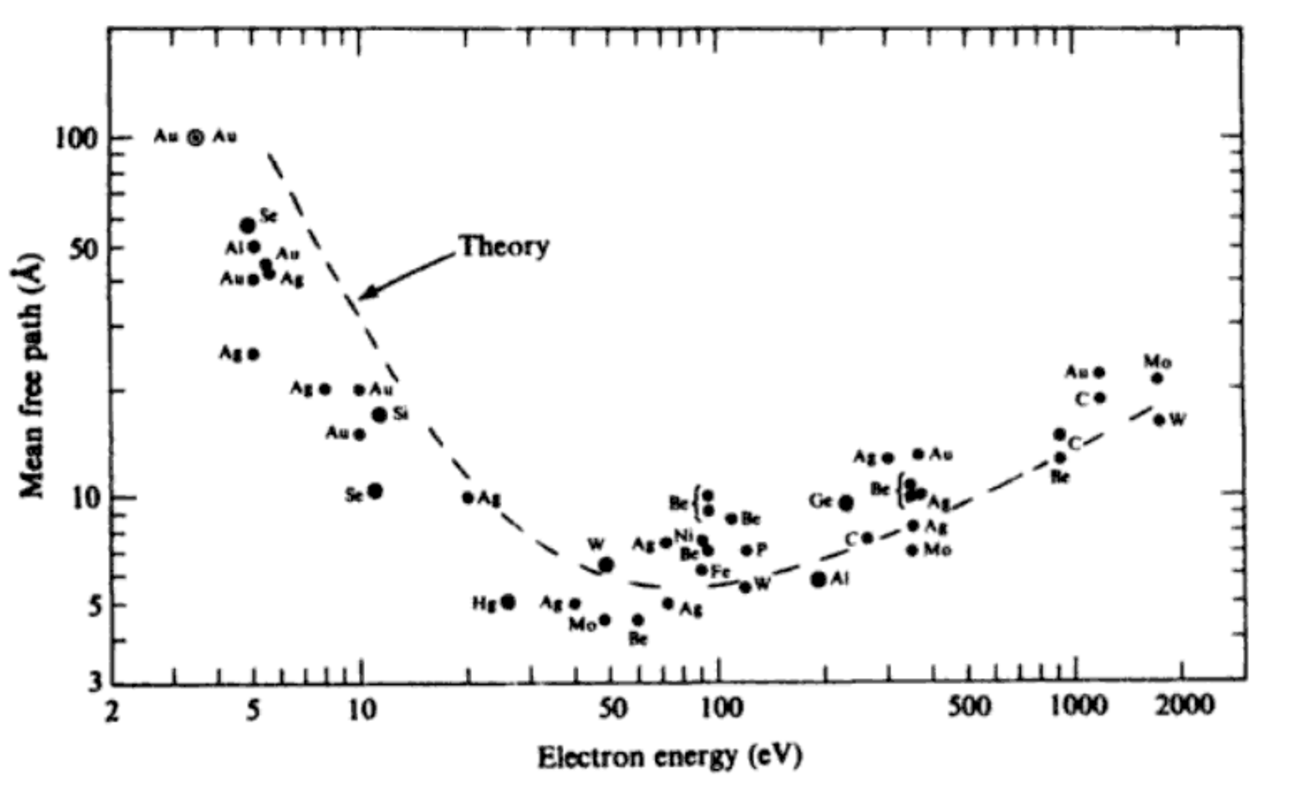
\includegraphics[scale=0.35]{figs/universalcurve.png}
\caption{Universal curve of electron mean free path in solids \cite{Zangwill}}	
\label{fig:univ-curve}
\end{figure}

\section{Low Energy Electron Diffraction}
When investigating the structure of bulk solids, diffraction is generally the most important tool; both photons and electrons are readily used as diffraction based probes of atomic structure. Analysis of diffraction through solid materials provides direct information about any translational or rotational symmetry present in the target material and thus can be easily used to characterize the structure of periodic crystalline materials. The study of crystallographic structure of materials dates back to the work of L. Bragg in 1913, who founded the field of X-ray crystallography \cite{Ashcroft}.

Crystalline solid materials exhibit high degrees of atomic ordering in three-dimensions with a specific periodicity in one or more directions. The surface of the solid represents a deviation from perfect infinite periodicity. Ideally the surface retains the same periodicity of the bulk solid structure, however, more often than not, the surface structure of a material contains significant deviations from the bulk structure. These geometric changes in atomic structure may result in interesting physiochemical changes in the material and thus are of particular interest for study.

\begin{equation}
\label{eq:lat}
\mathbf{R} = n_1 \mathbf{a_1} + n_2 \mathbf{a_2} + n_3 \mathbf{a_3}
\end{equation}


Solid materials can be described by the symmetry of their atomic structure. The Bravais lattice defines a purely geometric periodic array of lattice sites that house the repeated structure of the solid be that a single atom, group of atoms, or molecules. Equation \ref{eq:lat} defines the bravais lattice as all points with position vector, $\mathbf{R}$, with $\mathbf{a_n}$ representing basis vectors and  $n_n$ taking integer values \cite{Ashcroft}.

\begin{equation}
\label{eq:rlat1}
\mathbf{ b_i \cdot a_j} = 2\pi \delta_{ij}
\end{equation}

\begin{equation}
\label{eq:rlat2}
\mathbf{b_i} = 2\pi \frac{\mathbf{a_j \times a_k}}{\mathbf{a_i \cdot (a_j \times a_k)}} \text{  }\forall \text{ cyclic permutations of ijk}
\end{equation}

For every lattice defined by the set of primitive basis vectors, ${\mathbf{a_n}}$, there is a corresponding set of reciprocal lattice vectors, ${\mathbf{b_n}}$,  that generate the reciprocal lattice of the real space lattice.  These vectors have units of inverse length and thus can be considered to be the momentum space representation of the real space lattice. The reciprocal lattice plays a role in governing crystalline diffraction and a generalization of the law of conservation of momentum to discrete periodic lattices \cite{Ashcroft}. The reciprocal lattice basis vectors, ${\mathbf{b_n}}$, must satisfy the relations shown in Equations \ref{eq:rlat1} and \ref{eq:rlat2}. That the reciprocal lattice contains the same symmetry as the original real space lattice makes diffraction techniques, which are sensitive to the reciprocal lattice, able to provide real space information about precise atomic positions in the crystal.

Low energy electrons are distinctly qualified to probe the surface structure in solids for two primary reasons. First, as shown in Figure \ref{fig:univ-curve}, low energy electrons have minimal mean free path and thus will interact only with the first 3-5 atomic layers in a material. Finally the deBroglie wavelength of the electron is comparable to the interatomic distance in most solids, which allows for diffraction.

Electron diffraction is analogous to the theory of X-ray diffraction first described by L. Bragg, and is governed by the Laue equation, shown in Equation \ref{eq:laue}, describing the total change in wave vector of an electron after scattering. Here $\mathbf{K_{i}^{||}}$ and $\mathbf{K_{s}^{||}}$ represent the components of the wave vectors of the incident and scattered electrons parallel to the crystal surface and $\mathbf{g_{hk}}$ represent a reciprocal lattice vector of the crystal at the reciprocal lattice point denoted by (hk). The Laue condition then demands that in an electron scattering event, the total parallel component momentum transferred must be equal to a reciprocal lattice vector of the crystal. Using the Planck-Einstein relation for energy, the condition for elastic scattering, $E_i = E_s$, reduces to $|K_i| = |K_s|$. Here its worth nothing that the conservation of momentum, as implied by the Laue condition, $K_s^{||} = K_i^{||} - g_{hk}$ applies to electrons of any source, thus this condition describes the kinematics for low energy electron diffraction, Auger electron spectroscopy, as well as photoemission spectroscopy \cite{ SurfSciTechniques}. 

\begin{equation}
\label{eq:laue}
\Delta \mathbf{K^{||}} = \mathbf{K_{s}^{||} - K_{i}^{||}} = \mathbf{g_{hk}}
\end{equation}

The patterns formed by electron diffraction represent a scaled version of the reciprocal space lattice of the target crystal and thus contain information about translational and rotational symmetry in the real space system by the inverse transformation correlated with Equations \ref{eq:rlat1} and \ref{eq:rlat2}. While it is relatively straightforward to use LEED to derive the symmetry of the target crystal surface structure, it becomes more difficult to extract information regarding precise atomic positions relative to those predicted for the bulk structure. For this a more complex method of diffraction data analysis is employed, known as dynamical LEED intensity-voltage analysis, LEED-I(V).

In LEED-I(V), the energy of the incident electron beam is varied in discrete steps and the intensity, I, of various diffracted beams is analyzed as a function of the incident energy, V. This process requires additional hardware to capture images of the diffraction pattern for each step in energy of the incident electron beam, but the data extraction is relatively straightforward. For each energy step, an image of the diffracted beams is captured and saved digitally. One or more diffracted electron beams are selected in the images with an adjustable sized rectangular integration window. The total intensity of the beams in the window is summed and recorded. Finally this intensity is plotted as a function of the energy range of the experiment; optionally a local background can be subtracted from each data point for more accurate data. These intensity-energy curves contain information about the three dimensional structure of the diffracting material \cite{Hannon-LEEM-Book, vanHove-LEED, pendry-LEED}. 

In order to derive the atomic structure of the target material, a three -dimensional trial structure is provided to software packages that calculate the dynamic multiple scattering of incident electrons and predict the diffracted intensity as a function of incident energy. This computationally generated I(V) curve is then compared to the experimentally gathered I(V) curve. Then the trial structure is adjusted slightly and the process continues to iterate until reasonable agreement is found between the experimental data and computationally generated data. The last structure input to the process then contains the most accurate information about three-dimensional atomic positions in the target crystal. This structure can be compared to that of the known bulk crystal structure to analyze the presence of surface reconstructions and relaxations.


\section{Low Energy Electron Microscopy}
Low energy electron microscopy is a novel technique for rapid and robust surface science analysis. Electron microscopy dates back to the early 1930s and has evolved into a wide variety of analytic techniques. LEEM is a subset of cathode lens electron microscopy developed in principle in the 1960s while not fully realized until the 1980s after technological advances in vacuum technology and electromagnetic lens systems for electron optics. There are two primary features of LEEM that distinguish it from other forms of cathode lens microscopes, namely the energy regime of the incident beam and usage of the sample specimen as part of the lens system itself \cite{Hannon-LEEM-Book}.

LEEM can generally operate in two distinct modes by varying the probing source. In photoemission electron microscopy, (PEEM), a collimated beam of monochromatic photons is used to probe the sample surface and images of the surface are generated from photo-excited electrons. In LEEM mode, a collimated beam of low energy electrons in the range 0 to 100 eV is used to probe the surface region of the sample specimen. Analogous to LEED, low energy electrons are chosen specifically due to their high surface sensitivity as a direct result of their low mean free path. However, using low energy electrons as the primary beam poses many technological challenges. 
Lower energy electron beams are more susceptible to influence by external stray electromagnetic fields, which makes the electron beam difficult to control over large distances. To get around this challenge LEEM uses a high-energy electron beam in the range of 15 to 20 keV as the primary beam. The high-energy beam can be easily focused and manipulated using electromagnetic lenses.  The incident electron beam is only decelerated to very low energies just prior to interaction with the sample. This is accomplished by integrating the sample with the cathode lens. After passing through the objective lens, the high-energy electron beam experiences an approximately uniform retarding electric field from the cathode, which lowers the beam energy to the 0 to 100 eV range. The sample must be held at a high negative bias potential while simultaneously the space between the sample and objective lens must be very small in order to generate a strong electric field on the order of $10^6$ volts per cm \cite{Hannon-LEEM-Book}.

Using the sample as part of the cathode lens primarily restricts the types of samples available for study to non-insulating samples that are approximately flat. A sample that is overly rough or warped will cause the retarding field to be non-uniform thus reducing the overall resolution in the system as well as providing potential for sparks in the optics system between sample and objective lens. The high field requirements, sample conductivity, and macroscopic flatness prove to be minimal restrictions considering the advantages offered by LEEM analysis.

One of the most robust aspects of LEEM analysis is the ability to provide one tool that can image the sample in both real space and reciprocal space with high resolution. The objective lens of the LEEM system provides two focal planes that can be projected into the imaging column of the detection system. While operating in standard LEEM mode, the Gaussian plane of the objective lens provides a real space image of the sample surface with resolution better than 10nm parallel to the surface plane \cite{Hannon-LEEM-Book}. The back-focal plane of the objective lens can also be projected to the imaging column. This provides a direct image of the diffraction pattern or, said another way, records the angular distribution of the diffracted electron beams \cite{Hannon-LEEM-Book}.  Similarly in PEEM mode the Gaussian plane again provides a real space image generated by photo-emitted electrons, whereas the back-focal plane provides an image of the angular distribution of the photoemission process.

Reciprocal space images collected with a LEEM system are useful and distinct from conventional LEED imaging as a result of being able to drastically restrict the size of the incident electron beam. By introducing a limiting aperture into the illumination column, the spot size of the imaging beam can be restricted to sub-micron levels. To contrast this with conventional LEED, generally the illuminated area of the sample in conventional LEED spans multiple square millimeters \cite{Hannon-LEEM-Book}.
	
A second unique design in LEEM systems is the use of magnetic prisms to separate the incident and reflected electron beams by angular deflections. This allows the sample to be removed from the electron beam directly emitted from the electron source. In other words the sample is not required to be collinear with the electron source. This gives rise to a number of possible beam line geometries. An example of a standard LEEM beam line geometry is shown in Figure \ref{fig:LEEM-Geometry}. Having the sample removed from the direct line of sight of the electron source while also separating the incident and outgoing beams allows imaging of all reflected beams. 

In conventional LEED, the (0,0) spectrally reflected beam is not visible on the luminescent screen due to being blocked from view by the electron source. LEEM allows the spectral beam to be imaged directly along with emitted beams of higher angular order, however, in real space imaging, the surface image can only be formed by one  reflected beam at a time. Having the sample separated from direct line of sight with clever beam-line geometries allows LEEM to be implemented alongside other incident beams such as a molecular flux from a molecular beam epitaxy system (MBE). Thus LEEM can be used to image the real-time growth of thin films of a wide variety of materials atop a wide variety of substrates. This fact alone makes LEEM incredibly powerful and useful in the field of surface science. 
\begin{figure}
\centering
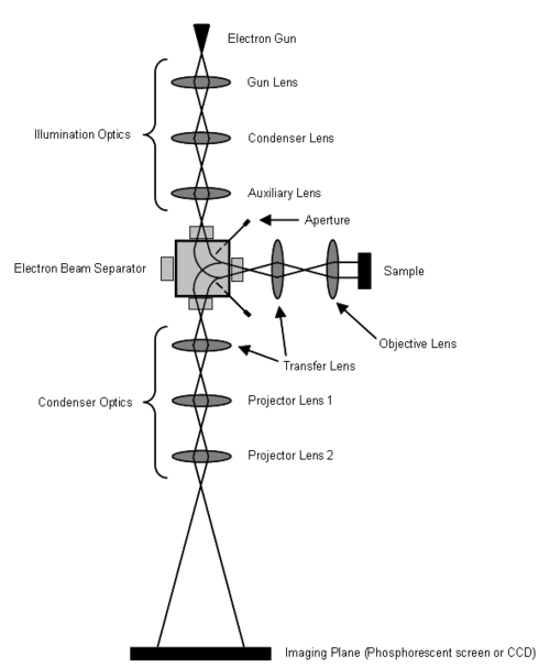
\includegraphics[scale=1.1]{figs/LEEMGeo-150.png}
\caption{Diagram of basic LEEM geometry. The sample is oriented at $\pm$90$^{\circ}$ with respect to the beam emitted from the electron source. Source from Brandon Howe: \protect\url{https://en.wikipedia.org/wiki/Low-energy_electron_microscopy}}
\label{fig:LEEM-Geometry}
\end{figure}
	
	The primary limits on the resolution in LEEM imaging come from aberration in the electron optics. The objective lens must have a small uniform aperture cut into its center in order to allow the incident and reflected beams to pass through it. This hole causes the field generated by the cathode to deviate from a ideal uniform field. Fringe effects from the aperture cause a divergence of the reflected beam after passing through the objective aperture. These aberrations are well understood and can be partially corrected through the use of an extra aberration correction that involves the installation of a second magnetic beam separator. This adds a significant cost to the device, yet also allows for an ultimate in-plane spatial resolution as low as 2 nm \cite{Hannon-LEEM-Book, Figuera-LEEM}. 

As LEEM continues to evolve as a powerful surface science tool, novel experimental techniques push the boundaries of LEEM's ultimate resolution while also granting access to new types of samples for imaging. By altering the electron source to provide polarized electrons, which have a fixed spin orientation, the magnetic domains in the sample surface can be probed with very high spatial resolution. This technique is known as Spin Polarized LEEM, SPLEEM. LEEM, along with many other electron microscopy methods, has a long history in the study of biological specimens \cite{Bauer-LEEM}. As biologic sciences advance, the need for rapid characterization techniques grows. One of the fundamental problems in modern biological science is characterization and sequencing of DNA samples in a rapid manner. This technique requires the ability to distinguish between different base pairs existing in individual DNA strands and is currently a cost-prohibitive technique \cite{MADLEEM}. A novel LEEM technique using a monochromatic aberration-corrected dual-beam LEEM system, (MADLEEM), seeks to utilize the high spatial resolution of LEEM to rapidly sequence DNA samples \cite{MADLEEM}.

LEEM's high spatial resolution within the plane of the sample surface can be extended to provide three dimensional mapping of atomic positions in the surface region through use of LEEM-I(V). LEEM-I(V), analogous to LEED-I(V), combines experimental data with computational modeling of dynamic electron scattering to generate a model of the atomic surface structure with very high resolution. Real space LEEM images represent maps of the local electron reflectivity in the surface. As the incident electron energy is changed, the local electron reflectivity also changes in ways uniquely linked to the physical and chemical properties of the local surface region.

LEEM-I(V) requires computational modeling to discern accurate information about the surface structure. A complicating factor for computational modeling of very low energy electron interactions is the treatment of the electron inner potential. For higher energy than LEEM operates at, the potential can be assumed constant. For very low energies, however, there is a complex energy dependence. Dynamical modeling of low energy electrons is an active area of current research. 

LEEM-I(V)  techniques are currently under study as a method for discerning the number of atomic layers in a sample with a high degree of spatial accuracy. This is useful for the study of novel layered materials such as graphene and other two-dimensional materials. As a result of thin film interference and/or quantum well resonance, the I(V) curves for layered materials show oscillations in the reflected intensity. These oscillations are inherently linked to the thickness of the material and thus to the number of layers \cite{Hibino}. Thus careful analysis of LEEM-I(V) data can elucidate the sample thickness for layered materials. This form of analysis, alongside software written to aid in data visualization and I(V)  data extraction, will be shown later as applied to a novel graphene system under study at UNH.
	
	
\section{Scanning Tunneling Microscopy: Ultra High Resolution Surface Microscopy}

STM is a form of non-optical scanning probe microscopy, which provides detailed mapping of the topography of a surface with atomic resolution. The mechanism of action, while relatively simple, relies on a purely quantum phenomenon called quantum tunneling, and thus STM has no classical analog. 

STM generates images by moving a finely pointed metal electrode across a sample while keeping the electrode-sample distance very small, on the order of a few Angstr\"oms. When a small bias voltage is applied between the STM tip and the sample, then electrons flow from tip to sample or sample to tip through the classically forbidden vacuum region. Classically, if the sample and tip are not touching then there is no flow of electrons due to not having a closed circuit. However, when the separation between tip and sample becomes so small that quantum physics begins to play a role, a current can flow whereby electrons tunnel through the vacuum region.

The amount of current crossing the classically forbidden region is exponentially dependent on the tip to sample distance. Thus, when the tip is closer to the sample surface more current flows and the opposite is true for larger tip to sample distances. Careful monitoring of the tunnel current coupled with the ability to precisely control the tip to sample distance via piezoelectric motors and a computer controlled feedback loop allows the STM to continuously read out a constant current. As the STM scans across the surface, the tip moves perpendicular to the surface plane so as to keep the tunnel current at a constant value. Thus the tip motion essentially traces out the topography of the sample surface; if the tip to sample distance is collinear with the z direction then the sample surface is in the x-y plane and the STM tip motion as a function of the position is a three-dimensional map of the surface structure, $z(x,y)$.

The simplest way to model the operation of an STM considers electrons tunneling through a one-dimensional barrier. The tip and surface can be considered for simplicity as two parallel metallic electrodes. The parameters needed to characterize the tunneling phenomenon in this model are the barrier height, $V_0$, the tip to surface distance, $s$, and the electron energy, $E$. Inside either of the two electrodes, the electron wavefunctions take on the form of traveling waves in the direction perpendicular to the surface plane, $z$, and are proportional to $e^{\pm i z}$. The vacuum region, represented by the one-dimensional potential barrier, is the classically forbidden region. In this region the electron wavefunction must decay, and thus the wavefunction inside the barrier region is represented by $e^{\pm \kappa z}$. Solving the Schr\"odinger equation yields the following relations for $k$ and $\kappa$ \cite{SPM-methods}:
\begin{equation}
k = \frac{[2 m_e (E - V_0)]^{\frac{1}{2}}}{\hbar}
\end{equation}
\begin{equation}
\label{eq:stm}
\kappa = \frac{[2 m_e (V_0 - E)]^{\frac{1}{2}}}{\hbar}
\end{equation}
Continuing the calculation and solving for the probability of an electron tunneling through the barrier yields the following exact solution for the transmission coefficient, $T$,\cite{SPM-methods}:
\begin{equation}
T = [1 + \frac{(k^2 + \kappa^2)}{(4k^2 \kappa^2)} \sinh^2{(\kappa s)}]^{-1}
\end{equation}
Taking the limit that the vacuum region should be strongly attenuating, i.e. $\kappa s >> 1$, the transmission coefficient simplifies to a more understandable term \cite{SPM-methods}:
\begin{equation}
\label{eq:stm2}
T \approx \frac{16k^2\kappa^2}{(k^2 +\kappa^2)^2}e^{-2\kappa s}
\end{equation}
In the approximate form for the transmission coefficient, it can be seen that the probability of an electron tunneling through the barrier depends exponentially on the tip to surface distance, s. Thus an STM can make high resolution maps of the surface by monitoring small changes in the tip to sample distance, which in turn cause large fluctuations in the tunneling current. A change of the tip to sample distance of 1{\AA} can cause a change in the measured tunneling current by roughly an order of magnitude \cite{SPM-methods, BinnigRohrerSTM}.

While the STM data can be considered a topographic map of the surface, the STM actually acts as a probe of the local density of electronic states in the surface. Depending on the direction of the bias voltage applied between the tip and sample, electrons will either tunnel from the sample into the tip or the tip into the sample. In the first scenario, electrons tunnel from the sample to the STM tip; electrons from the highest occupied electronic states in the sample will tunnel into the STM tip filling the lowest unoccupied electronic states. In this case the STM image represented by $z(x,y)$ provides a three-dimensional map of the local density of the highest occupied electronic states in the sample. In the second scenario, electrons from the highest occupied electronic states in the STM tip tunnel into the lowest unoccupied electronic states of the sample. Thus the STM image represented by $z(x,y)$ now provides a three-dimensional map of the density of lowest unoccupied electronic states in the sample surface region. The magnitude of the applied bias voltage affects also affects which electronic states are capable of contributing to the total tunnel current \cite{STM-I}. STM tips are generally chemically etched such that they are as sharp as possible. The tip sharpness and the high sensitivity of tip to sample distance make STM a uniquely local probe. These two characteristics combine to allow the ultra high-resolution surface structure measurements.

The tip to sample distance is an important factor in why STM images provide high spatial resolution. Since the probe of the surface is an electron, one should consider the wavelength of the electron at a typical energy for STM operation to understand limits of resolution. However, since STM operates with tip to sample distances on the order of a few {\AA}ngstr\"oms, this distance is less than that of the electron wavelength. For example using the relation between the de Broglie wavelength in Angstr\"oms and electron energy in electron volts, 
\begin{equation}
\lambda(E_{eV}) = \frac{12.3}{E^\frac{1}{2}} {[\text{\AA}]}
\end{equation} you find for a 1.5eV electron a wavelength of roughly 10 {\AA} \cite{Ashcroft}. This wavelength would in general not allow for resolution of any surface features smaller than the wavelength, such as atomic separation distances, which are on the order of 3{\AA}. STM is not bound by the Fraunhofer diffraction limit of electron wavelength because the tip to sample distance is lower than the electron wavelength \cite{SPM-methods}, and thus the STM operates in the near-field regime.  This makes STM uniquely qualified as a microscopy technique for detailed structural analysis requiring atomic precision.

Besides providing topographic information of the sample surface, STM can collect data in a number of other operational modes. Equations \ref{eq:stm} and \ref{eq:stm2} demonstrate the functional dependence of the tunneling current on the local tunneling barrier $V_0$. The local tunneling barrier is related to the work function of the two electrodes in the tunneling system. Thus STM can be used to investigate changes in work functions of materials at a highly local scale \cite{STM-I}. STM is also frequently operated in one of a number of spectroscopic modes known as scanning tunneling spectroscopy, STS. As mentioned previously, the local tunneling barrier height is related to the tip to sample distance and also the work functions of the two electrodes. By scanning the tip across the sample but at each sampling point also collecting a measurement of current as a function of tip height for varying values of the tip height, then the local tunneling barrier can be extracted from a semilog plot of tunneling current versus tip to surface distance.
\begin{equation}
\label{eq:stm3}
I \propto \int_{0}^{eV} \rho(E) T(E,V) dE
\end{equation}

Many modes of spectroscopic operation for STM have been developed. Generally these modes seek to decouple the geometric and/or topographic information in the STM images from the electronic information. STS allows information about the density of electronic states to be recorded more accurately by recording how the tunnel current changes with bias voltage as a function of bias voltage, $\frac{dI}{dV}(V)$. This quantity is proportional to the density of states in the surface region to first order \cite{SPM-methods}. While many different STS techniques are capable of elucidating the electronic properties of the surface, they come with added drawbacks. STS experiments that map the electronic structure of the sample surface as a function of energy and spatial position require repeated scans of the exact same area of the surface with high precision. This makes thermal fluctuations in the system as well as chemical changes to the scanning probe incredibly important to control \cite{SPM-methods}. Thus extracting spectroscopic data generally requires a low temperature STM, well prepared samples, well prepared tips, and excellent vacuum conditions.


However, if one is only concerned with analysis of the general topographic structure of the sample surface region, then low temperatures are not needed and standard STM images provide the needed information. The work detailed later utilizes room temperature STM to analyze the surface structure of a novel graphene system in comparison to the well-known structure of graphene grown epitaxially on the ruthenium surface.

\section{Further Surface Science Techniques}
Before a sample is ready to study with STM, the surface must be adequately prepared and characterized to ensure that it is free of contamination. One of the major limitations of STM is the lack of distinct chemical sensitivity. While STM images may display surface defects and surface contaminants in the form of adatoms or clusters of atoms, there is no direct signal to specify the type of atom being imaged. Auger Electron Spectroscopy is a surface sensitive technique, which measures the relative elemental composition in the surface region. By illuminating the surface with a collimated beam of electrons, electron emission from the surface can be stimulated as a result of the Auger scattering process. This process can be modeled in three steps. 

The first step is ionization of an atom by the incident electron beam. Here so long as the incident beam has sufficient energy, $E \approx 2keV$, a core level electron in the surface atom will be emitted. Since the first step results in an excited electronic state for the surface atoms, the second step is relaxation. Here a higher shell electron will transition to the core vacancy. The final step is Auger emission. In this step the transition energy of step two is imparted to another non-core electron in the surface atom. If this energy is larger than the electron binding energy, the second electron will be emitted from the atom as a free electron.

The Auger process clearly requires atoms with multiple electrons, thus as a result, Auger Spectroscopy is insensitive to hydrogen and helium. The Auger process can be characterized by the electron level of the core electron and the two levels of the higher shell electrons. The process is denoted using the spectroscopic notation for the energy levels involved, thus for example, a common Auger process involves a core electron from the K energy level and two electrons from the L energy level and is denoted as a KLL transition. The kinetic energy of the emitted electron can be calculated as $E_K - (E_{L1} - E_{L2})$ where $E_K$ is the energy of the core electron, $E_{L1}$ is the energy of the electron that fills the core vacancy, and $E_{L2}$ is the energy of the emitted electron's energy level.

Since the energy of the emitted electron depends on the exact energy levels of the atom it came from, the kinetic energy of the electron contains chemical information. Thus by illuminating a sample with a collimated beam of electrons and carefully measuring the energy of emitted electrons, the elemental composition of the surface can be accurately measured to within a few percent. This is extremely beneficial when preparing a sample for further analysis via LEED and STM. An example of the Auger spectrum recorded from a ruthenium crystal is shown in Figure \ref{fig:auger-ru}.

\begin{figure}
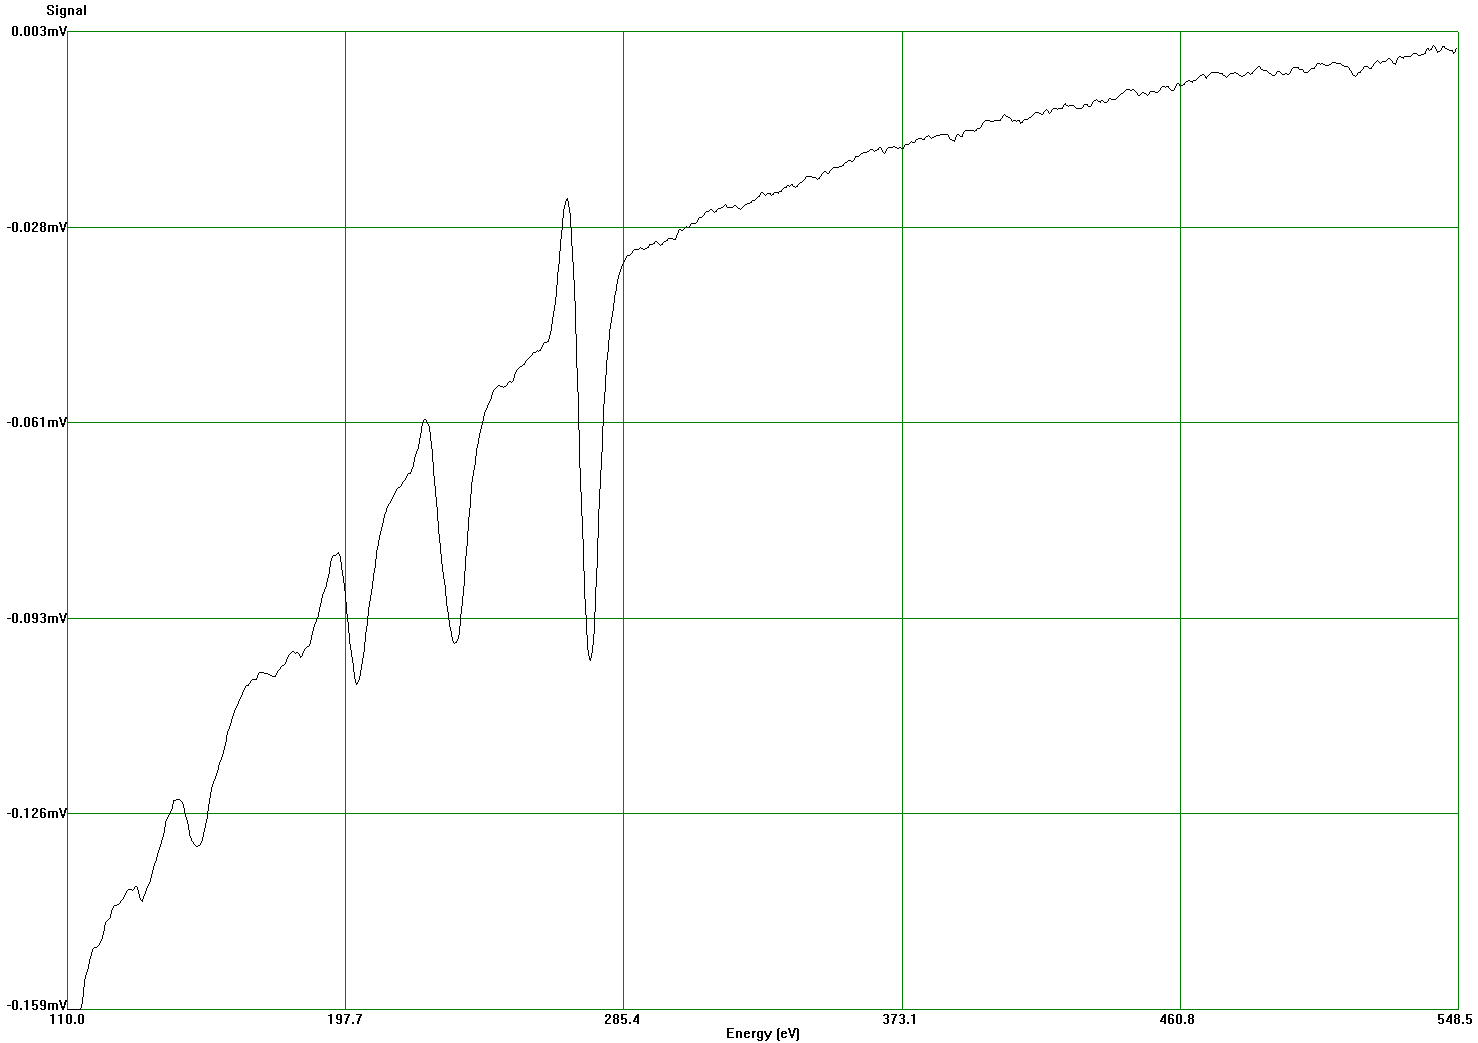
\includegraphics[scale=0.42]{figs/auger-ru.png}
\caption{
An example auger electron spectrum collected from a ruthenium single crystal. The peak at 272 eV is the primary peak for the ruthenium auger spectrum. The primary electron energy is 1.5 keV.
}
\label{fig:auger-ru}
\end{figure}

\section{Summary}
The following surface science studies of a novel graphene system and other layered materials make use of the following tools: AES for characterization of the sample contamination levels, LEED for characterizing the crystalline properties of the sample at the macroscopic scale, STM for analyzing the surface topography at the nanoscale and finally LEEM and micro-LEED to analyze the structure of the surface with high resolution to better understand the atomic structure and layer thickness.

% ------------------- %
% Chapter Name
\chapter{\sc Polymorphic Graphene: Modulating the Graphene Surface Structure}
\label{ch:Polymorphic Graphene}
\section{Graphene on Ruthenium: a departure from pristine graphene}

Chapter 2 discussed the properties of graphene in its ideal form, a perfect two-dimensional hexagonal crystalline lattice of carbon atoms. However, when graphene is grown on various substrates its material properties and structure can manifest in drastically different ways. Graphene growth on metallic substrates has been widely studied and generally the properties of the system can be separated into two categories: systems with weak carbon-metal interaction, such as graphene on gold, and systems with strong carbon-metal interaction, such as graphene on ruthenium \cite{batzill, graphene-metals}.

\begin{figure}

\centering

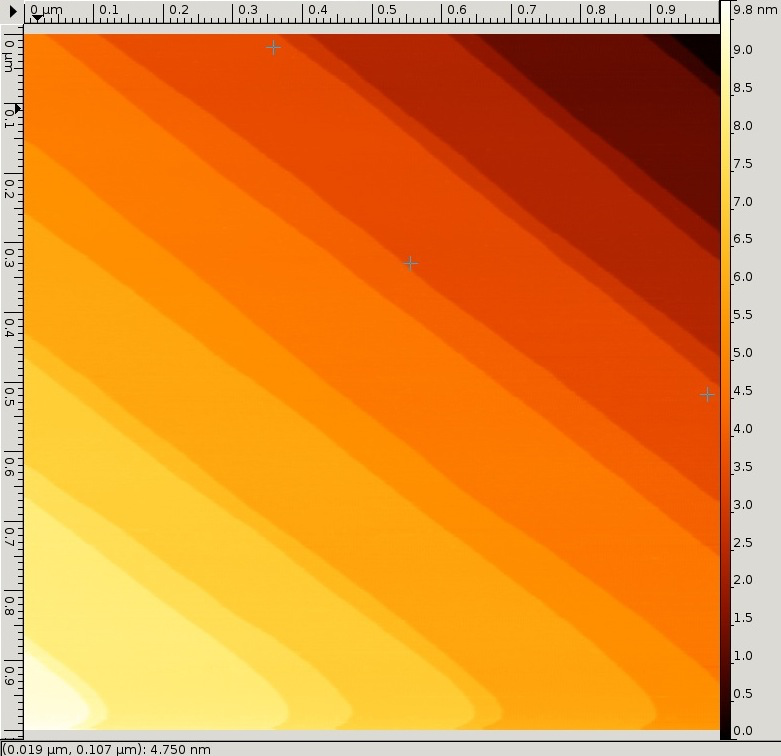
\includegraphics[scale=0.5]{./figs/ru-stm-clean.png}

\caption{
STM image showing the surface of a well prepared ruthenium (0001) single crystal. The surface exhibits atomically flat terraces separated by monatomic steps. Image dimensions are 1$\mu$m x 1$\mu$m.
}
\label{fig:ru-stm-clean}

\end{figure}

Ruthenium is a transition metal with a hexagonal crystal structure and lattice constant of 2.7 {\AA}. The most common applications for ruthenium are principally restricted to electronic use as a hardening agent in electrical contacts as well as a resistive material in its native oxide state, \ce{RuO_2} \cite{ru-electronics, ru-resistors}. However, ruthenium is also used in smaller quantities for catalytic properties as well as in some novel dye-sensitized photovoltaic applications \cite{ru-solar}. The (0001) surface of ruthenium consists of atomically flat terraces with hexagonal surface symmetry terminated by monatomic steps where the atoms in the lower terrace have a $180^{\circ}$ rotation relative to the top terrace. A large scale STM image of a clean ruthenium surface is shown in Figure \ref{fig:ru-stm-clean}.

The most common lattice defects in ruthenium crystals constitute oxygen, sulfur, and carbon. All non-carbon defects can be easily removed from the crystal via prolonged high temperature annealing \cite{ru-auger-prep}. Carbon, however, is not removed in this cleaning process and thus additional methods are required to prepare a pristine ruthenium single crystal. Two methods are commonly employed to prepare pristine ruthenium. First, the crystal may be cleaned by repeated cycles of ion sputtering and annealing. Generally argon ions are used as the sputtering agent. This method leaves the surface area free of contaminants but also has a tendency to leave subsurface pockets of argon atoms, which are visible in STM images. If sputtering is not used, then carbon can be removed from the ruthenium bulk by repeated cycles of exposure to oxygen followed by high temperature annealing. This process works as a result of the variability of carbon solubility in the ruthenium crystal as a function of temperature.

At elevated temperatures, the bulk carbon solubility drops, resulting in a diffusive flow of interstitial carbon atoms from the bulk region to the surface. When the surface is exposed to oxygen, carbon atoms bond with oxygen atoms to produce \ce{CO} molecules. Upon annealing, the carbon monoxide molecules desorb from the surface to vacuum. Thus repeated cycles of oxygen exposure and annealing will deplete the bulk crystal of carbon contaminants. This process can be monitored with Auger electron spectroscopy in order to determine the relative carbon concentration in the crystal. The Auger signal for carbon in ruthenium crystals is somewhat complicated compared to the other contaminants due to the strong overlap between the ruthenium signal and carbon signal near 273 eV. By examining the differentiated auger spectrum, a clean ruthenium sample is characterized by a roughly symmetric peak and trough near 273 eV whereas a largely carbon contaminated sample will manifest with a largely reduced peak and extended trough at 273 eV \cite{ru-auger-prep}. 

\begin{figure}
\centering
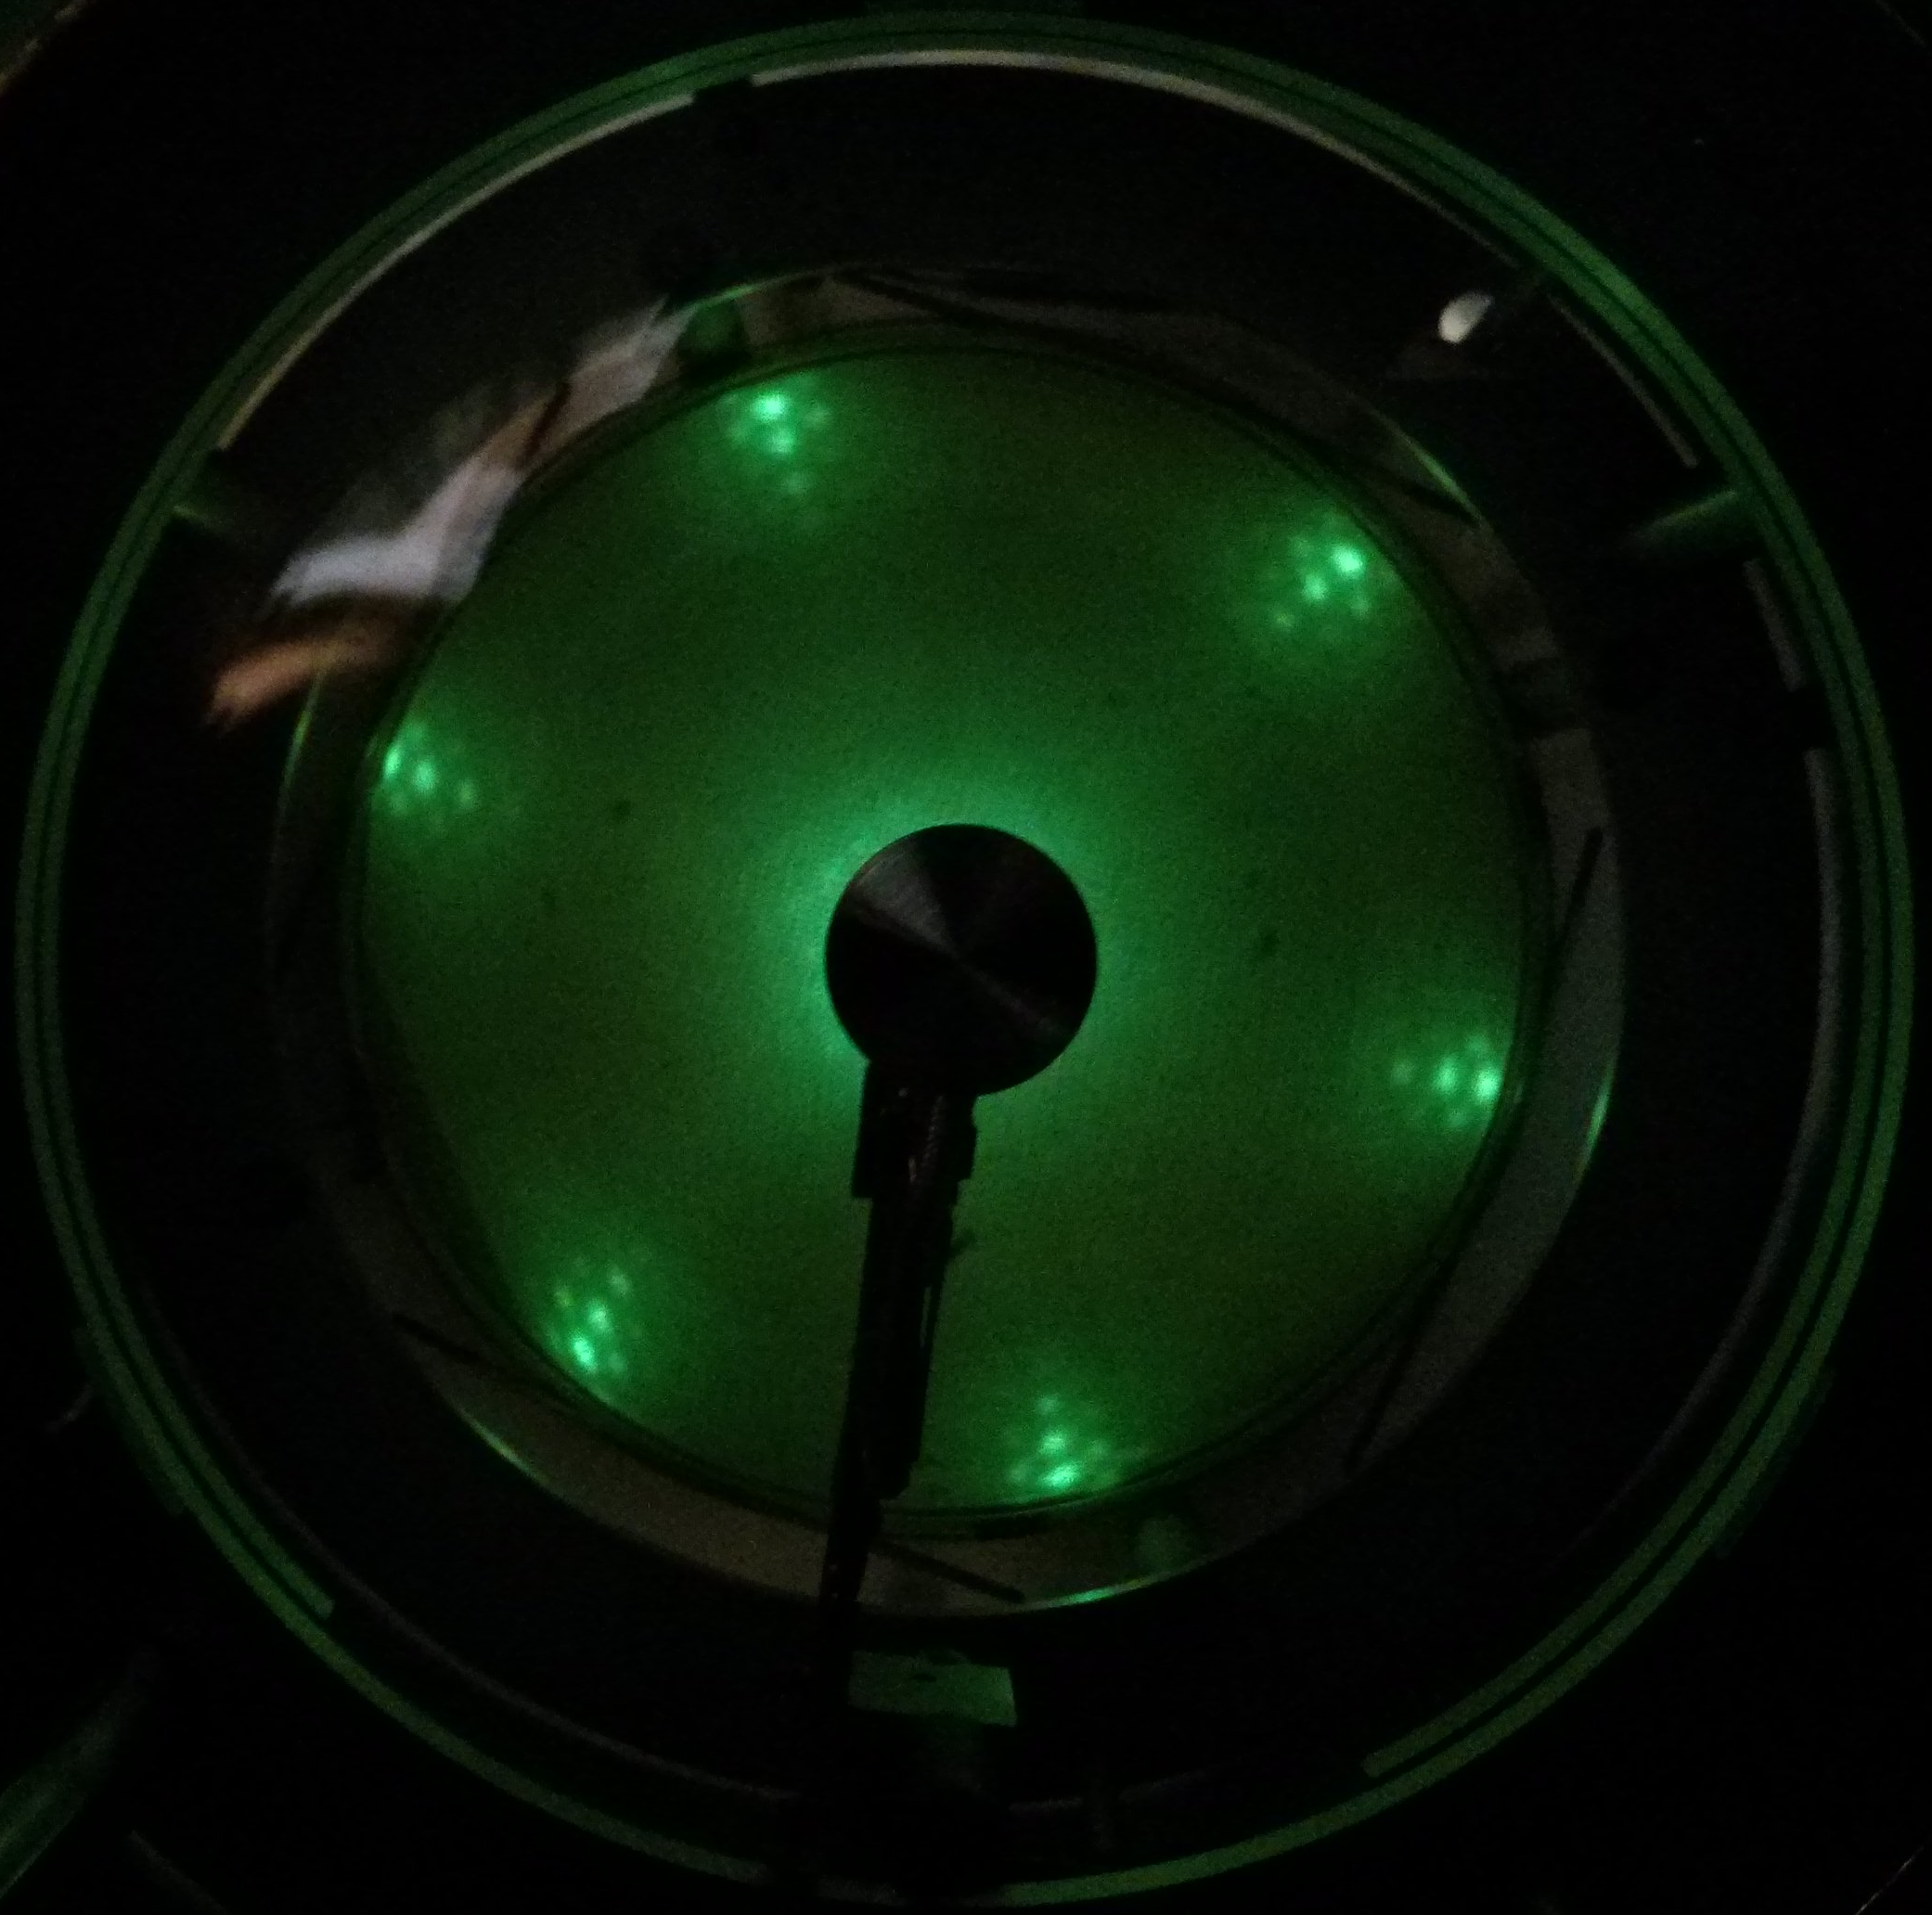
\includegraphics[scale=0.20]{./figs/graphene-ruthenium-leed.png}
\caption{
LEED pattern of the graphene/ruthenium system displaying characteristic satellite peaks surrounding the primary ruthenium (1x1) pattern. Image collected with incident beam energy of 62 eV. The bright diffraction peaks in the center of the outer hexagons represent the ruthenium p(1x1) pattern. The surrounding diffraction spots, referred to as satellite peaks, indicate the presence of the moire superstructure. 
}
\label{fig:graphene-leed}

\end{figure}


A clean ruthenium (0001) crystal can be characterized by an auger signal displaying only strong ruthenium peaks with little contribution from oxygen, carbon, and sulfur. A sample Auger spectrum with from clean ruthenium can be seen in Figure \ref{fig:auger-ru}; the primary peak is roughly symmetric at 273 eV indicating low carbon contamination and the oxygen peak at 512 eV is negligible.  Furthermore, for a clean ruthenium crystal, the LEED pattern will display only a (1x1) primary hexagonal structure, which will be visible in conventional LEED between 50 - 60 eV. If residual oxygen is present in the system from the cleaning cycles, it will be easily visible as a p(2x2) LEED structure. Residual surface carbon from cleaning cycles or from prolonged high temperature annealing can also be clearly distinguished by its LEED signature.

Surface carbon on ruthenium (0001) readily forms graphene islands via a two-step process. When a diffusive flow of carbon is driven from the bulk to the surface by thermal annealing, the carbon atoms first manifest as surface adatoms in a disordered phase. Continued annealing drives the transition from amorphous carbon adatoms to an ordered graphene phase. In this process carbon atoms join into rings forming a graphene structure. However, it should be noted that the growth process of graphene on ruthenium is not as simple as the process on other materials. At the ruthenium surface there is a large energy barrier inhibiting the transition of carbon adatoms into ordered graphene \cite{c-clusters}. LEEM and DFT studies attribute this barrier to the change in height when transitioning from a carbon adatom to a carbon atom in a graphene sheet above the surface \cite{c-clusters}. Instead of a direct transition, it is energetically favorable to form clusters of five carbon atoms that then combine with the graphene sheet edge. This type of growth process is characteristic of metal-carbon systems exhibiting strong metal-carbon bonds, such as graphene on nickel \cite{c-clusters}.

The combination of a hexagonal graphene surface layer atop the hexagonal ruthenium crystal results in an interesting phenomenon known as a moire structure. Both crystal systems are hexagonal and have similar but not perfectly matched lattice constants, with a percent difference of roughly 9\%. As a result of the lattice mismatch, the graphene layer does not lie flat atop the ruthenium surface. Instead, a rippled periodic superstructure forms. The rippled carbon surface also causes pronounced changes in the atomic positions of the uppermost ruthenium surface layers; the uppermost ruthenium layers also exhibit rippled deviations from their normal bulk positions \cite{sxrd}.  The size of the superstructure can be revealed by its reciprocal space pattern imaged with LEED \cite{graphene-metals}. 

The moire structure in LEED for the graphene/ruthenium system is characterized by sharp satellite peaks that form a hexagon surrounding the primary substrate peaks as shown in Figure \ref{fig:graphene-leed}. The ratio between the primary substrate hexagonal reciprocal lattice constant and the satellite peak reciprocal lattice constant is reported to be 11.6 \cite{graphene-metals}. This implies that the periodic superstructure has a real space periodicity of approximately 12 graphene unit cells. Counting the number of ruthenium lattices that would fit in the same distance yields approximately 11. Thus the superstructure is denoted as a 12 x 11 structure where the repeating unit is a hexagonal combination of 12 x 12 graphene unit cells on top of 11 x 11 ruthenium unit cells. This periodic superstructure has a real space periodicity of 2.98 nm, which corresponds to the peak-to-peak distance of the ripples in the graphene layer; the moire period can be easily verified with STM line profile analysis.  The notation for graphene superstructures can be generalized to (n+1) x n indicating a superstructure with n+1 graphene unit cells atop n ruthenium unit cells. Finally it should be noted that the LEED patterns generated from the graphene/ruthenium system show very minimal rotational disorder between the graphene layer and the ruthenium layer. Systems with weaker metal-carbon bonding exhibit a large amount of rotational disorder between the graphene sheet and the substrate surface. Due to the size of sampling area in conventional LEED, these features manifest as ring and arc structures in the LEED pattern \cite{graphene-metals}. 
\begin{figure}
  \centering
  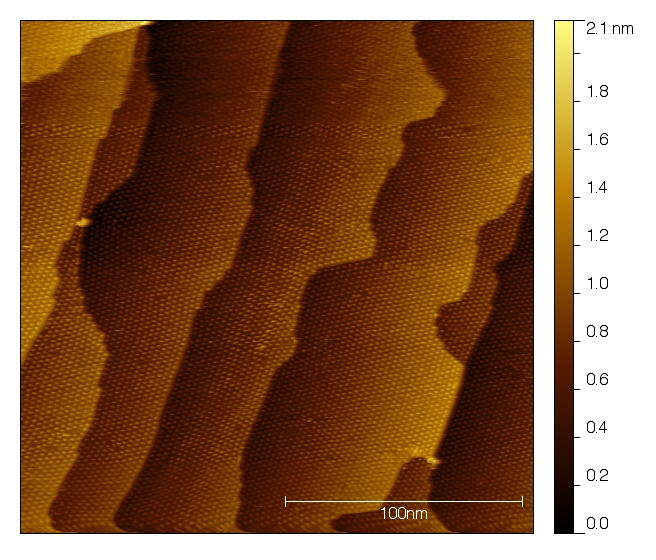
\includegraphics[scale=0.7]{./figs/graphene-ruthenium-stm.png}
  \caption{
  STM image displaying characteristic moire pattern formed by graphene grown atop Ru(0001). The graphene sheet grows in a uniform manner across the monatomic steps in the ruthenium surface.
  }
  \label{fig:ru-graphene-long}
\end{figure}

The graphene/ruthenium system is ideal for the study of graphene on metals as a result of the ease of growth for the carbon adsorbate layers on the ruthenium surface. The moire reconstruction of graphene on ruthenium is easily reproducible with the same periodicity and generally independent of the common growth methods. Graphene on ruthenium grown by CVD, PVD, or graphitization will nearly always adopt the same structure with minimal rotational disorder. Furthermore, this system exhibits a high degree of long range ordering with the graphene sheets growing in a uniform manner across the stepped ruthenium surface for multiple microns up to millimeter scale graphene \cite{ mm-graphene}. Figure \ref{fig:ru-graphene-long} shows a typical STM image of the graphene ruthenium surface with long range order and the characteristic moire structure easily visible as the series of bright and dark spots.

\begin{figure}
  \centering
  \includegraphics[scale=0.7]{./figs/atomic-graphene.png}
  \caption{
  Atomically resolved image of the graphene/Ru(0001) system. The moire unit cell is denoted by the black lines in the figure. The bright spots represent the high points of the corrugated structure.
  }
  \label{fig:atomic-graphene}
\end{figure}


The graphene ruthenium moire pattern appears in STM images as a rippled hexagonal superstructure. The peak-to-peak distance, the moire period, can be measured using line profile analysis and is generally consistent with the reported value of 2.98 nm \cite{march}. The moire structure, as imaged by STM, is a physically corrugated system, that is to say the corrugation is not purely an electronic effect such as fluctuation in charge density. The rippled structure can be considered to be made up of areas of varying carbon-ruthenium interaction strength. The peaks in the STM represent area where the carbon atoms are more weakly bound to the ruthenium surface and thus sit higher from the surface. The low points in the structure represent areas with stronger overlap between the graphene $\pi$ orbitals and the ruthenium $4d$ orbitals. As a result, it has been reported that close up STM images of these two regions appear different. In the peaks of the structure, where the carbon atoms are less strongly bound, atomically resolved STM should image all atoms within the graphene rings. In the low regions, where carbon atoms are strongly bound to the surface, the STM images only every other atom in the graphene ring \cite{march}. An atomically resolved room temperature STM image of graphene on ruthenium is shown in Figure \ref{fig:atomic-graphene} with the unit cell of the moire superstructure also denoted. In this image there is not sufficient detail to resolve differences between the imaged atoms in the high sites compared to the low sites of the moire unit cell. Imaging a smaller area and/or imaging at low temperature may resolve this discrepancy.

Graphene grows epitaxially atop the ruthenium surface with relative ease and forms highly ordered uniform sheets with the characteristic rippled structure. The resulting moire structure is independent of the method of growth, CVD, PVD, or graphitization all result in the same structure. However, if graphene is to be utilized as a scaffold for the growth of other materials, then control over the surface structure may be desired. Also its worth nothing that since the moire structure is closely linked to the bonding between the carbon layer and the ruthenium surface, its possible that modulations of the surface structure may induce unique changes in the electronic structure of the graphene-ruthenium system, however, those changes are beyond the scope of the present research. By altering the graphene growth process we have shown that it is possible to form many different moire structures simultaneously and the resultant material is hereby denoted as polymorphic graphene.

Multiple polymorphic graphene samples have been prepared in our combined UHV growth and analysis chamber; the growth of polymorphic graphene results in distinct signatures visible by LEED and STM indicating differences from the standard model of graphene on ruthenium. The primary difference between standard growth of graphene on ruthenium and the growth of polymorphic graphene is the presence of an atmosphere of atomic hydrogen near the sample surface during the carbon deposition.

\subsection{Growth of Polymorphic Graphene}

Physical vapor deposition growth of polymorphic graphene samples begins with preparation and analysis of the underlying Ru(0001) substrate. The ruthenium crystal is depleted of contaminants by repeated cycles of annealing at 1200 K in a moderate atmosphere of molecular oxygen followed by rapid heating to temperatures above 1800 K to remove residual surface oxygen. This process is repeated until the Auger spectrum indicates a crystal free of sulfur, oxygen, and a sufficiently low carbon concentration. At this point the LEED pattern should have only a sharp Ru p(1x1) pattern. If a p(2x2) pattern is visible then likely the surface is still partially oxidized and heating to 1800 K or higher for 20 seconds should desorb all remaining oxygen. The carbon source for PVD is prepared by outgassing overnight before a beginning the growth procedure. The source will remain clean once outgassed until the next time the system has been vented.


\begin{figure}
  \centering
  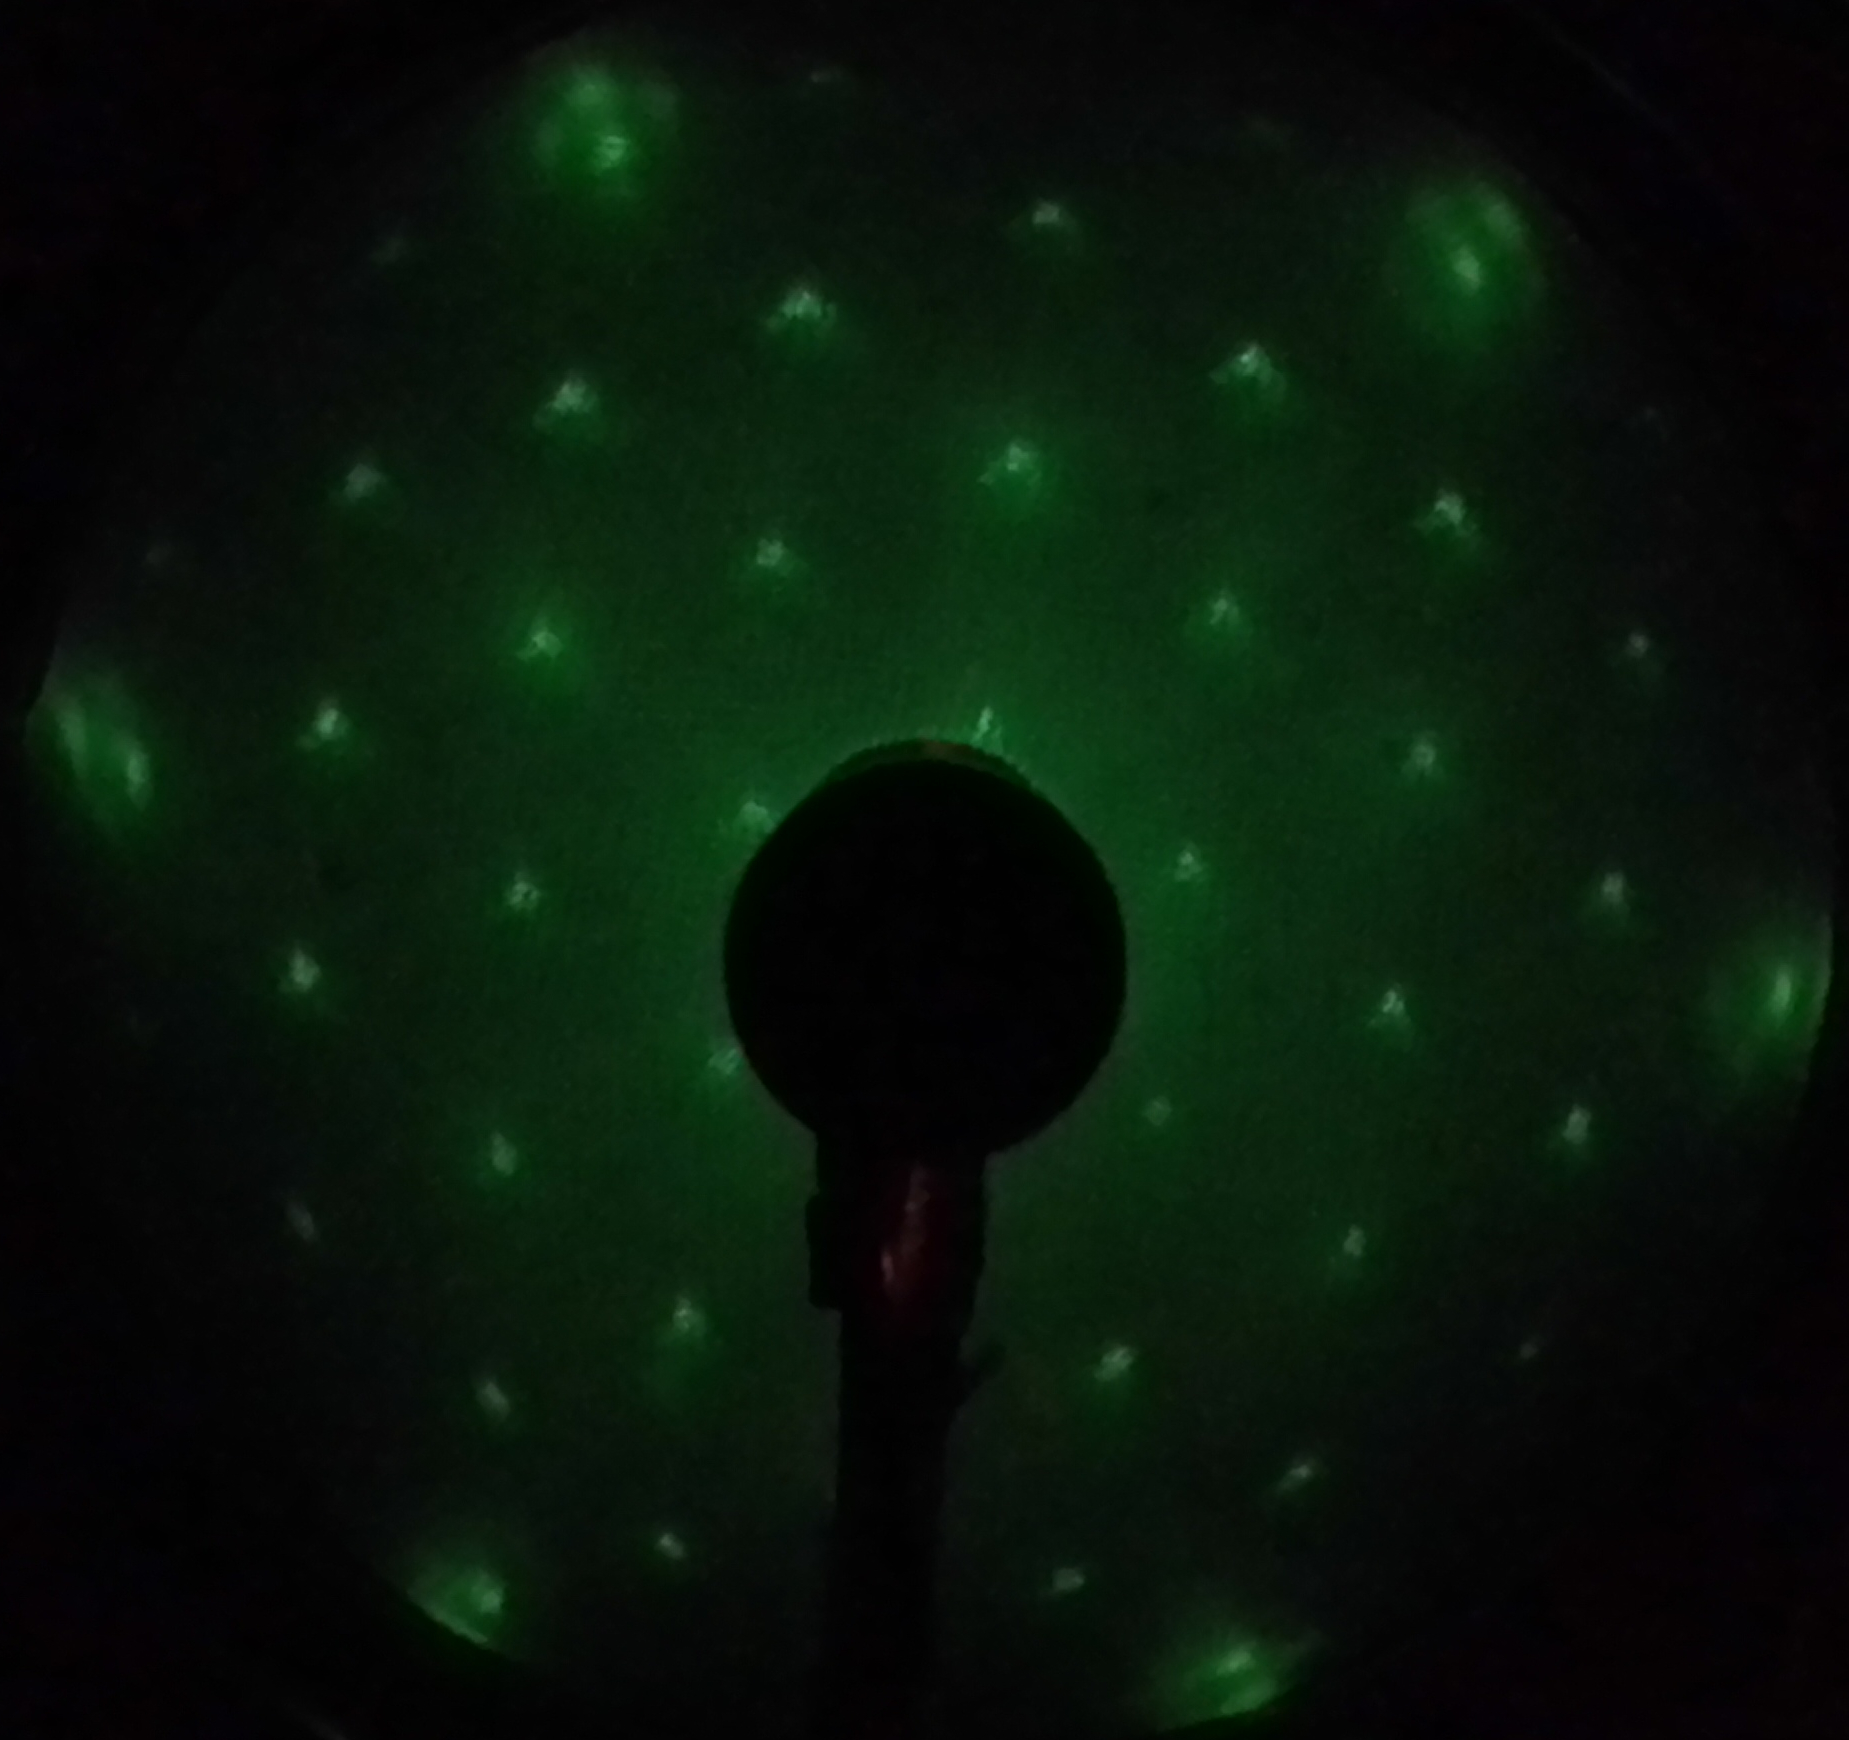
\includegraphics[scale=0.2]{./figs/graphene-hydro-leed.png}
  \caption{
  LEED pattern obtained after a growth of polymorphic graphene on a ruthenium (0001) substrate. Compared with Figure \ref{fig:graphene-leed}, there are many extra diffraction peaks. These peaks form a $(2\sqrt{3}$ x $2\sqrt{3})$R$30^\circ$ pattern relative to the primary Ru (1x1) pattern.
  }
  \label{fig:graphene-hydro}
\end{figure}

The temperature of the crystal and the carbon source are both crucial parameters for the growth process. The carbon source must be hot enough to sublimate carbon atoms to the ruthenium crystal surface as well as hot enough to fracture a hydrogen gas molecule. The temperature of the carbon source can be monitored with an optical pyrometer, whereas the temperature of the ruthenium crystal is monitored both by an optical pyrometer and a C-type thermocouple spot welded to the side of the crystal. The sample crystal should be brought as close to the carbon source as possible; direct line of sight between the carbon source and the sample presents a flux of carbon atoms to the ruthenium surface. A smaller distance between the sample and the source also serves to maximize the local atmosphere of atomic hydrogen gas.

With the sample positioned close to the carbon source, the temperature of the crystal is raised to near 800K by heating with a tungsten filament mounted behind the crystal. After a slight period of preheating the sample, the carbon source is brought up to temperatures above 1800K. At this point the UHV chamber is backfilled with ultra high purity molecular hydrogen to a pressure between $3$x$10^{-7}$ and $1$x$10^{-6}$ torr. The hot carbon source acts as a fracturing element for the atmosphere of molecular hydrogen gas thus creating a local atmosphere of atomic hydrogen in close proximity to the sample surface. This results in an incident flux of carbon atoms and atomic hydrogen onto the ruthenium surface.

The co-deposition process can be carried out for anywhere between 30 to 90 minutes. After halting the deposition, the LEED pattern can be assessed, however, generally an annealing cycle must follow the deposition to generate a clear LEED pattern. After the deposition, the sample is annealed at 1200-1225 K until a clear LEED pattern is obtained. This entire process may need to be repeated several times to achieve the desired sample quality. 

\begin{figure}
  \centering
  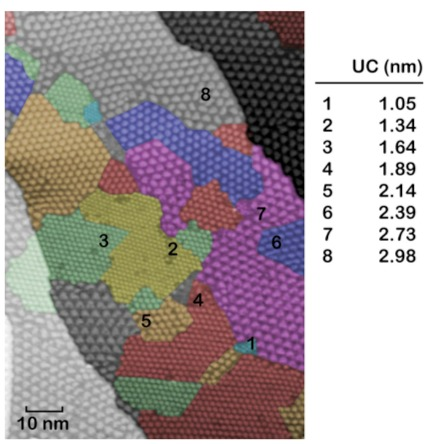
\includegraphics[scale=0.8]{./figs/moires.jpg}
  \caption{STM image displaying multiple domains of graphene with differing periodicity. Eight separate domains, each with a different moire period, are false colored for clarity.}
  \label{fig:polygraphene}
\end{figure}

\section{Polymorphic Graphene: A modulated graphene structure}

The signature of polymorphic graphene can be seen in multiple ways after the deposition. The first indication that the sample is distinct from the standard graphene ruthenium system comes from analysis of the LEED pattern. After co-depostion of atomic hydrogen and carbon, additional LEED spots forming a $(2\sqrt{3}$x$2\sqrt{3})$R$30^\circ$ pattern relative to the Ru p$(1$x$1)$ pattern are visible but often very faint in intensity. The relatively low intensity of the additional LEED spots may indicate that the sample quality is low or that the area exhibiting polymorphism is small. Figure \ref{fig:graphene-hydro} shows the LEED pattern exhibiting extra diffraction peaks alongside the primary ruthenium and moire peaks. Auger spectroscopy confirms that there are no additional contaminants in the sample surface region, thus it can be concluded that the presence of additional LEED peaks stems from the addition of hydrogen to the growth process. Given that conventional LEED displays the reciprocal space LEED pattern averaged over a large sample area, it can not be directly concluded what $(2\sqrt{3}$x$2\sqrt{3})$R$30^\circ$ pattern represents with respect to the physical structure of the system. Thus further analysis of the system is required.

\begin{figure}
  \centering
  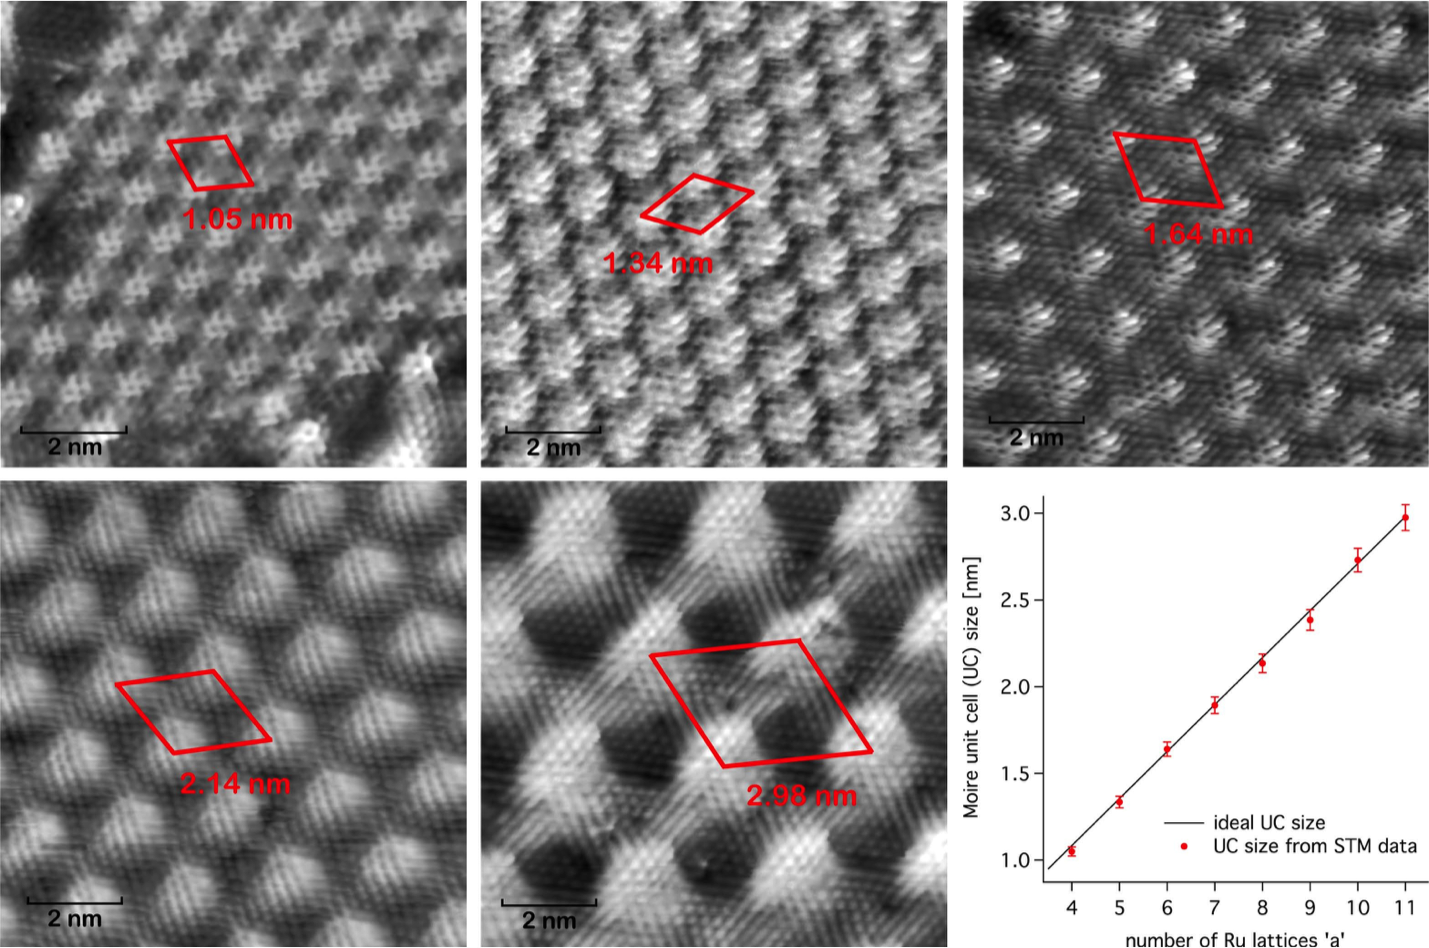
\includegraphics[scale=0.68]{./figs/unit-cell-plot.png}
  \caption{
  Atomically resolved STM images of polymorphic graphene. Domains with different unit cell sizes are shown with a unit cell overlay. Bottom Right: Plotting Moire unit cell size against the number of ruthenium lattices which fit in each unit cell length displays a linear relationship. 
  }
  \label{fig:unit-cell-plot}
\end{figure}

The second indication of structural deviation from the standard graphene/ruthenium system comes from analyzing STM images from the sample surface. STM analysis reveals numerous distinct domains in the graphene surface with a wide range of moire periods. Previously, only moire domains of 2.98 nm and 2.4 nm have been reported from STM investigation of graphene on ruthenium \cite{march, vazquez}. STM images of polymorphic graphene grown using the aforementioned procedure display morie unit cell sizes ranging from 1 nm to the standard value of 2.98 nm covering many values in between but never larger than 2.98 nm. An analysis of moire unit cell sizes observed compared with the number of ruthenium unit cells which fit in a given moire unit cell shows a linear relation between moire unit cell size and number of ruthenium unit cells. This implies that each consecutive moire superstructure corresponds to an increase of superstructure size by one single ruthenium unit cell. Using the previously defined nomenclature for describing the graphene/ruthenium superstructure, this relationship is quantified as follows: for a given moire structure with unit cell size, $a_n$, corresponding to a superstructure consisting of n+1 graphene unit cells atop n ruthenium unit cells, the next largest moire structure will have a moire period of $a_{n+1}$ and a superstructure denoted by n+2 x n+1.

There is some discrepancy as to the exact size of the moire superstructure in the graphene ruthenium system. DFT studies suggest there is little difference energetically when modeling the system as 12x11, 11x10, or other similarly sized superstructures \cite{graphene-metals}. Measurements from conventional LEED generally cannot distinguish between the difference in a 12x11 structure or an 11x10 structure. Taking the ratios between the two observed reciprocal lattice vectors will lead to a value somewhere in between 11 and 12 \cite{graphene-metals}. However, a surface x-ray diffraction, SXRD, experiment remedies the discrepancy with convincing evidence that the true periodic structure in the graphene/ruthenium system is larger by a factor of two \cite{sxrd}. The suggested model for the superstructure is split into four moire sublattices with a total size of 25 graphene unit cells atop 23 ruthenium unit cells. This model can then be envisioned as made up of four of the previously mentioned superstructures if they are accepted to have a superstructure size of 12.5 x 11.5. Using this model, the graphene superstructure is described by n+2 graphene unit cells atop n ruthenium unit cells, (n+2 x n).

\begin{figure}
  \centering
  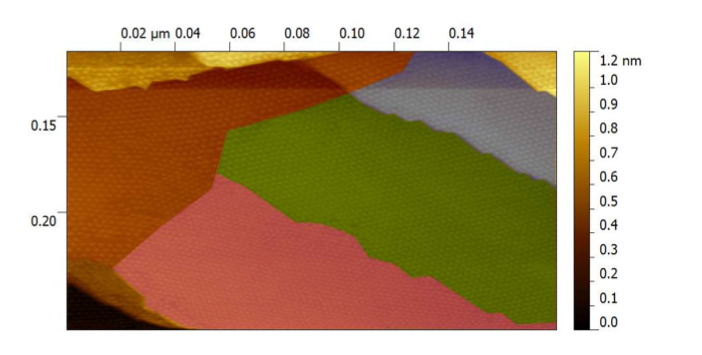
\includegraphics[scale=0.72]{./figs/half-integer-structures.png}
  \caption{
  STM images false-colored to show domains with differing moire periodicities. The green domain has a moire period of 2.56 nm, which corresponding to a (22 x 20) total superstructure consisting of four inequivalent subcells with periods of 2.56 nm. 
  }
  \label{fig:moire25}
\end{figure} 

During STM investigation of a polymorphic graphene sample, additional domains were discovered, which did not fit correctly in the old model for the superstructure size. Figure \ref{fig:moire25} displays a polymorphic graphene domain with a moire period of 2.56 nm. Comparing this value to the plot of unit cell size against number of ruthenium lattices shown in Figure \ref{fig:unit-cell-plot}, its clear that a unit cell size of 2.56nm would have corresponded to fractional values of the total number of ruthenium unit cells contained in the superstructure. A moire period of 2.56 nm would correspond, using the old model, to a (10.5 x 9.5) superstructure. Using this larger scale model suggested by SXRD for the total moire structure, we can fit STM observations of additional moire sizes, which were incompatible with the previous model. If instead the (n+2 x n) model is used, which generates a superstructure size of (25 x 23) for the standard graphene/ruthenium system, then the 2.56 nm moire structure fits a (22 x 20) superstructure that consists of four inequivalent cells with unit cell size of 2.56 nm.

\section{Limitations in analysis of polymorphic graphene}

A number of open questions remain concerning the growth and properties of polymorphic graphene, some of which are beyond the scope of this thesis work, however others will be explored in further chapters. Chief among the list of questions is addressing the role of hydrogen in the polymorphic graphene system. The STM images of the polymorphic graphene surface demonstrate the prospect of modulating the surface structure of the graphene/ruthenium system at the atomic level. The growth process for polymorphic graphene allows many moire domains to nucleate which would be otherwise energetically disfavored. Analysis of the surface of polymorphic graphene with atomic resolution shows little difference from the standard graphene/ruthenium system aside from the change in moire period. From the STM images the possibility that the surface of the graphene system contains hydrogen can be ruled out. In other words, the growth process is not forming graphane, the hydrogenated form of graphene, at least when viewed from the top down. 

One of the limitations of STM characterization is that the imaging technique is only sensitive to the topmost surface layer. Thus while the polymorphic graphene system can be imaged with atomic precision, there is a lack of understanding of the structure of the system below the carbon surface. Comparison of LEED patterns and STM images of standard graphene/ruthenium systems to the polymorphic graphene/ruthenium system show staunch differences, thus the hydrogen modulation of the growth process must play an important role. However, with STM and conventional LEED alone, no data can be obtained as to the role the hydrogen plays in the nucleation of different graphene domains.

Furthermore, STM investigation of the system does not easily provide information concerning the thickness of the carbon layer or layers at the surface. Thus it is not known whether single layer, bilayer, or many layers of graphene are grown atop the ruthenium surface. As mentioned in Chapter 3, low energy electron microscopy, LEEM, allows the surface of a crystal to be imaged simultaneously with an epitaxial growth process. It has been shown that LEEM provides a unique way to observe the nucleation of graphene islands and further growth into large scale graphene sheets atop the ruthenium surface \cite{mccarty-carbon, c-clusters}. Using this method, determination of the layer thickness is relatively straightforward given that the nucleation of each subsequent layer can be observed in real time. There is, however, one major limiting factor that makes using this technique to characterize polymorphic graphene growth more difficult. Currently polymorphic graphene growth happens at mid to high vacuum levels with relatively high pressures of hydrogen gas used relative to the base pressure of a LEEM system. Furthermore, currently polymorphic graphene growth has only been tested using a PVD growth process using a solid carbon source. These two properties of the growth process make integration with a LEEM system difficult, however it may be possible to adapt the growth of polymorphic graphene to a CVD, MBE, or segregation growth process more suitable to integration with LEEM. Chapter 5 will explore an alternative method for addressing the question of carbon layer thickness in the polymorphic graphene samples.

As mentioned before, STM can provide atomic scale images of only the upper most surface layer in the system. No other information concerning atomic positions subsurface is available. It may be of interest to have a better understanding of the precise atomic reconstructions present in polymorphic graphene as applied to the entire superstructure as a whole. To do so, information is needed about the positions of the ruthenium atoms within the supercell as well as the hydrogen. There are a limited number of surface science techniques available that can provide atomic scale information regarding the three dimensional position of atoms in the system with resolution small enough to probe individual domains in the polymorphic graphene system. Chapter 3 discussed LEED-I(V) as one potential tool for mapping atomic positions in a crystalline solid. Specifically LEED-I(V) carried out in a LEEM system has the possibility to restrict the electron beam sample area to sub-micron levels. Thus $\mu$-LEED-I(V) is an ideal candidate for further study of the polymorphic graphene system.

Finally, there are a number of open questions about the properties of polymorphic graphene, which are beyond the scope of this work but may warrant future studies. Specifically this work has focused on the structural characteristics of the polymorphic graphene system and their differences when compared to the standard graphene/ruthenium system. Given that the electronic properties of a material can be inherently linked to the structure of the material, it is quite possible that polymorphic graphene exhibits distinct electronic properties compared to the standard graphene/ruthenium system.

Pristine freestanding graphene is known to be a zero-gap semiconductor with extraordinarily high conductance. However, single layer graphene on ruthenium should depart from freestanding graphene significantly due to the strong overlap in the moire low regions between the graphene $\pi$ orbital and the ruthenium $4d$ orbital. This strong binding should disrupt the structure of graphene $\pi$ bands. Polymorphic graphene, however, may exhibit properties closer to pristine graphene as a result of the hydrogen in the system due to similarities with other graphene systems involving hydrogen. 

Silicon carbide is one of the most commonly used substrates for the study of graphene due to ease of growth. One common technique to prepare large-scale high quality graphene sheets involves the graphitization of 6H-SiC (0001). When a single carbon layer is grown in this manner, it remains strongly bound to the SiC surface, and as such is commonly referred to as a buffer layer, since it will not exhibit graphene like properties. However, it has been shown that when this system is exposed to a flux of atomic hydrogen, the hydrogen atoms penetrate the carbon surface layer and bind strongly at the SiC interface \cite{ SiC-passivation}. This is a result of the numerous dangling bonds present at the SiC interface. The hydrogen atoms passivate the SiC surface, which has a number of results. First it drastically reduces the total surface energy at the interface between SiC and the carbon buffer layer. Finally, the carbon buffer layer is lifted up higher from the SiC surface and becomes very weakly bound to the surface. Thus this process of hydrogen passivation transforms the strongly bound carbon layer into what is now called quasi-freestanding epitaxial graphene.

The graphene/ruthenium system may have a similar reaction to hydrogen intercalation. Initially there is strong bonding between carbon and ruthenium in the low points of the moire superstructure. The corrugated moire superstructure also presents many ruthenium dangling bonds at the interface between the ruthenium surface and the carbon layer. When atomic hydrogen is introduced into the system its possible that the hydrogen penetrates the carbon surface and remains bound at the interface between ruthenium and graphene. It has been previously mentioned that there is no indication found of hydrogen atop the carbon surface layer. Thus if hydrogen remains present in the system after the growth process, it must be at least subsurface relative to the uppermost carbon layer. If the atomic hydrogen manifests at the carbon-ruthenium interface, then it should be expected that the carbon surface layer is lifted higher from the ruthenium surface in a similar manner to the silicon carbide system. If this is the case then it can be expected that the electronic properties of this system will be different from those of the standard graphene/ruthenium system as a result of weaker overlap between the passivated ruthenium and carbon. These properties could be explored in the future using a combination of scanning tunneling spectroscopy, STS, and micro spot sized angle resolved photoemission spectroscopy, $\mu$-ARPES, to better understand the density of states and band structure of the system. ARPES measurements have been carried out for the graphene/ruthenium system before and after intercalation of atomic oxygen and the results are similar to those of the graphene/SiC system when exposed to atomic hydrogen \cite{o2-intercalation}. 





% Chapter Name
\chapter{\sc A Low Energy Electron Microscopy Investigation of Polymorphic Graphene}
\label{ch:A Low Energy Electron Microscopy Investigation of Polymorphic Graphene}

\section{Preliminary LEEM investigation of polymorphic graphene}
In order to more fully characterize the polymorphic graphene system, further surface science tools beyond conventional LEED, AES, and STM are required. In collaboration with the Center for Integrate Nano-Technology, CINT, at Sandia National Laboratory in Albuquerque, NM, a preliminary study of the polymorphic graphene system has been conducted using a low energy electron microscope. To begin this study, a polymorphic graphene sample was prepared at UNH using the method outlined in Chapter 4.

A small section of the sample surface area was found to display the characteristic conventional LEED signature of polymorphic graphene. Minimal other characterization was performed at UNH before packaging the sample for transit. The sample was transported to Sandia while still mounted within its UHV sample holder, however an additional solid washer was installed above the sample surface to prevent contact to the sample surface during transit.

Upon arrival at the CINT facility at Sandia, the sample holder assembly was disassembled so the ruthenium crystal could be mounted on the LEEM system sample holder. During this step it was crucial to keep track of sample orientation so that a specific area on the sample could be found during LEEM analysis. At this point it was noted that the ruthenium crystal had a distinct crack and warp on one section of the crystal, which made for an easy reference point, however this sample feature would have other important implications later in the study. Since the sample was transported to Sandia in air, it was necessary to perform a significant outgassing step under high vacuum before a LEEM investigation could be started. During this phase the sample was heated to 200$^{\circ}$ C by a rear mounted filament and allowed to outgas for some few hours. The pressure in the preparation chamber rose to over $10^{-8}$ torr at this point, indicating a high amount of outgassing from the sample.

\begin{figure}
  \centering
  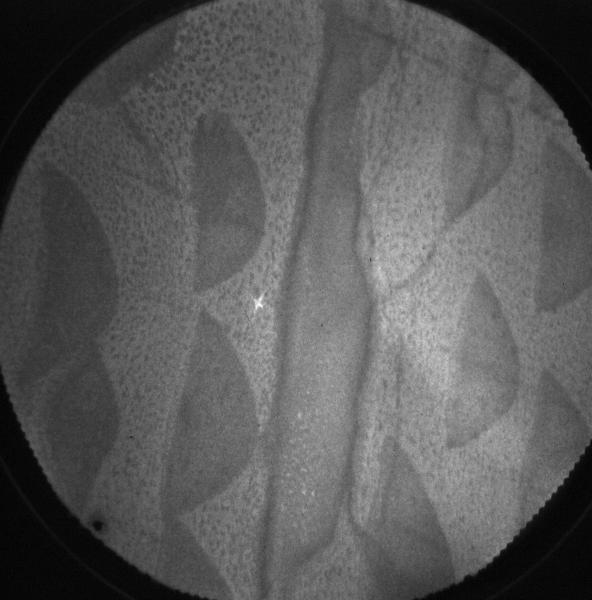
\includegraphics[scale=0.75]{./figs/LEEM-islands.jpg}
  \caption{
  Real Space 50 $\mu$m FOV LEEM image of the graphene/ruthenium system displaying characteristic lens shaped graphene islands, which appear as darker islands atop a brighter background. Image collected with incident beam energy of 13.9 eV. Data shown is part of a LEEM-\textit{I(V)} data set collected with 0.1 eV energy steps between images. Most islands are 3-5 $\mu$m at max width.
  }
  \label{fig:LEEM-islands}
\end{figure}

Upon initial investigation with real space LEEM using a 50 $\mu$m FOV, areas of the sample containing lens shaped islands were readily visible. These areas were identified as graphene islands and matched well with other reported studies of the graphene/ruthenium system using LEEM \cite{sutterleem}. Knowing the FOV of the LEEM images was 50 $\mu$m, the size of the graphene islands could be estimated to be multiple microns at their widest points. Here the relative coverage of graphene on the Ru(0001) surface can be estimated quickly due to the fast imaging nature of LEEM. The experiment demonstrated that samples could be grown ex-situ and transported to Sandia for imaging with minimal preparation needed before data collection.

\begin{figure}
  \subfloat[Real space LEEM image at 0.5eV incident energy with 50 micron FOV \label{subfig1}]{
    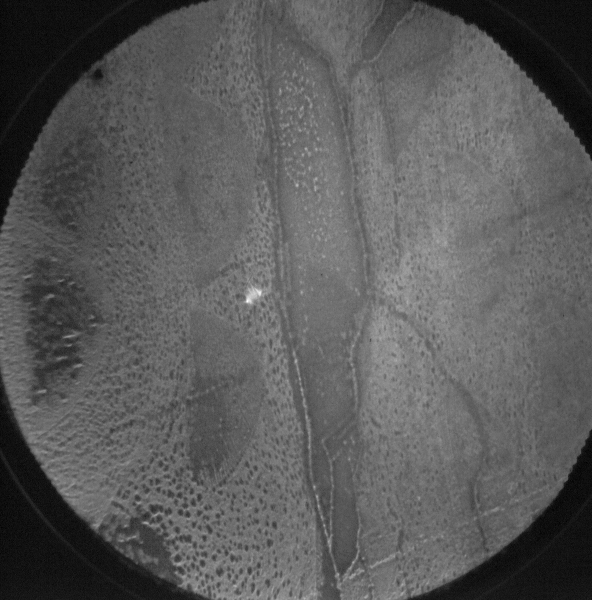
\includegraphics[scale=0.5]{./figs/mLEED1.png}
  }
  \hfill
  \subfloat[Aperture limited real space LEEM image \label{subfig2}]{
    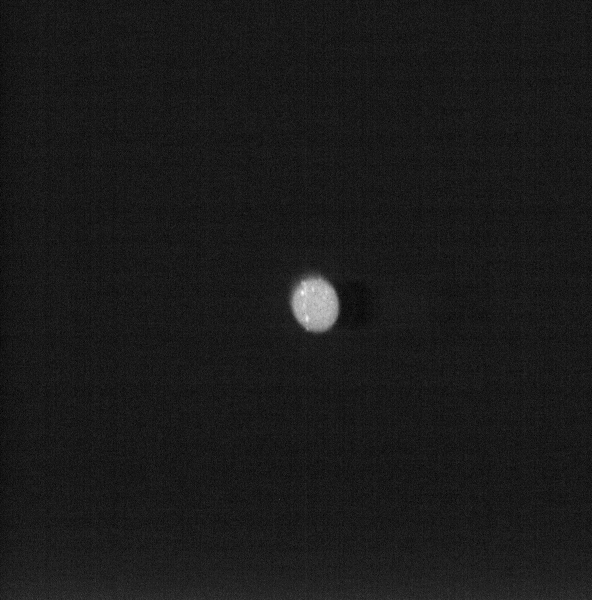
\includegraphics[scale=0.5]{./figs/mLEED2.png}
  }
  \\
  \subfloat[Overlay of (a) and (b) with 40\% transparency showing which part of the sample is imaged to acquire the data shown in (d) \label{subfig3}]{
    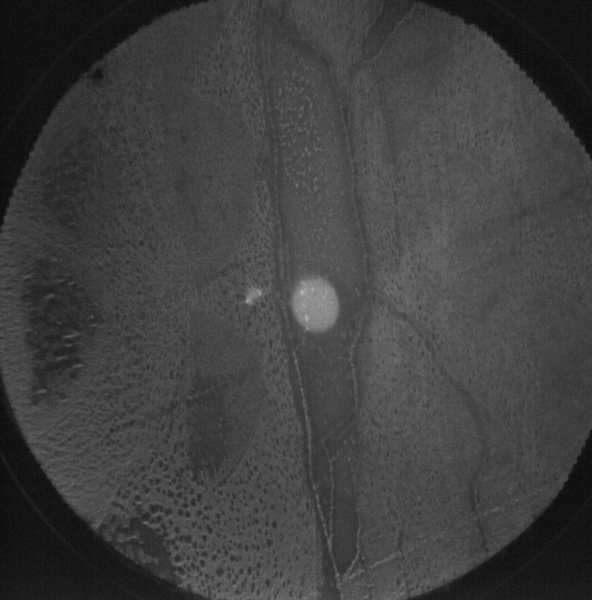
\includegraphics[scale=0.5]{./figs/mLEED3.png}
  }
  \hfill
  \subfloat[$\mu$-LEED image from roughly 5 micron illuminated section of sample. Reciprocal space image acquired at 50.0 eV. Ru (1x1) peaks are visible along with carbon satellite peaks typical of the graphene/ruthenium system.
                \label{subfig4}]{
    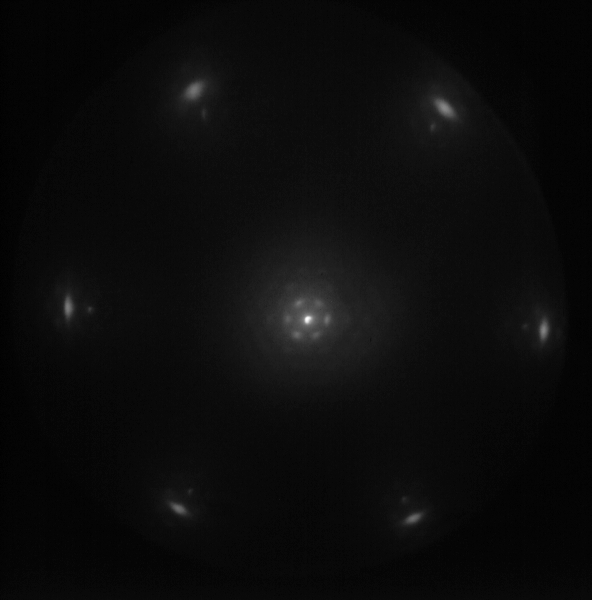
\includegraphics[scale=0.5]{./figs/mLEED4.png}
  }
  \caption{
  The $\mu$-LEED process shown where a specific location on the sample can be selected for acquisition of reciprocal space data. This process is sometimes referred to as selected area low energy electron diffraction.
  }
  \label{fig:microleed}
 \end{figure}

Further investigation of the sample at Sandia using $\mu$-LEED imaging was carried out in sample regions with visible graphene islands. The $\mu$-LEED technique allowed for a very high degree of control concerning which areas of the sample were imaged in reciprocal space by using micron sized apertures. To do so a large area real space LEEM image was acquired first so that areas of interest could be located. In this investigation we sought to image the graphene islands as well as the surrounding area with reciprocal space mapping. At this point a beam-limiting aperture was positioned in the beam line of the reflected electron beam after exiting the objective lens system before entering the transfer lens to the imaging column. This restricted the acquired image of the electron beam spot to a fixed diameter. With the aperture in place, a second real space image was collected such that only data from within the beam spot was acquired. By overlaying both real space images atop one another using post-processing software, the exact spot on the sample can be seen where reciprocal space data was collected.

Using the above technique, $\mu$-LEED patterns were collected from graphene islands as well as the surface between the islands. The LEED data was collected using a 5 $\mu$m aperture. Thus data was collected from an area on the sample illuminated by an approximately circular electron beam spot with roughly five micron diameter. Figure \ref{fig:microleed} shows an example of a real space LEEM image with graphene islands, an aperture limited real space image, the overlay of the two images together, and finally the LEED pattern acquired at a fixed energy from the spot illuminated in the images. The observed $\mu$-LEED patterns do not show evidence of extra diffraction peaks as were observed using conventional LEED at UNH. This is likely attributed to the limited area on the sample that was discovered to display polymorphic characteristics when characterized at UNH. Due to time restrictions and further experimental complications, the exact position of the sample that displayed polymorphic signatures could not be located.

\begin{figure}
  \centering
  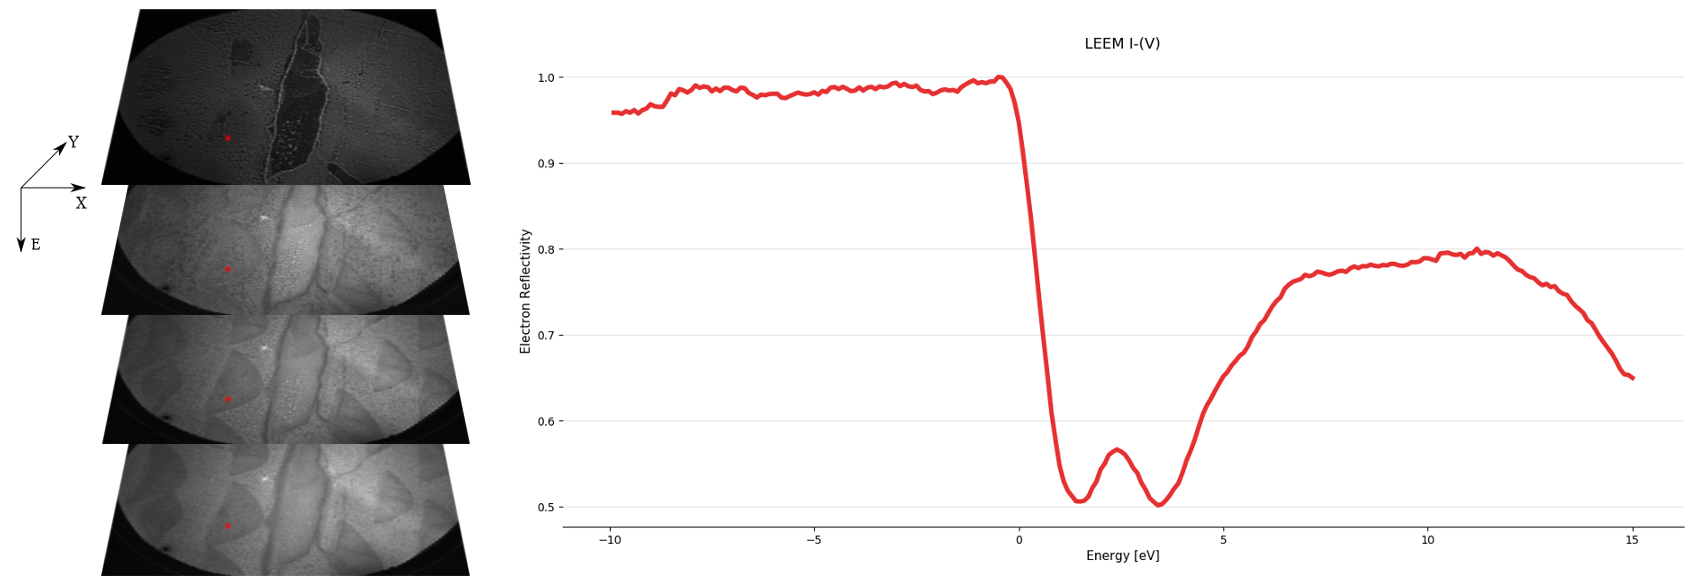
\includegraphics[scale=0.55]{./figs/IVDiagram.png}
   \caption{
  Example of a LEEM-\textit{I(V)} data set. A sequence of 250 real space images (left) are stacked vertically according to the incident electron energy at which the image was acquired. The energy step between images is 0.1 eV. \textit{I(V)} curves (right) are extracted by selecting the pixel intensity from a single pixel (highlighted in red) in each image sliced vertically through the energy axis. The structure of the curves relates to the three-dimensional structure of the sample material.
  }
  \label{fig:LEEM-I(V)-Example}
\end{figure}

Aside from the $\mu$-LEED patterns collected from the sample, a second data set using real space images was collected to allow for intensity-voltage (LEEM-\textit{I(V)}) analysis of the graphene/ruthenium system at very low incident energy. Specifically, this type of data set was of interest to look for a signature of carbon layer thickness. With STM analysis, measuring the exact layer thickness is difficult and slow. Due to the rapid imaging nature of LEEM, there is potential to quickly determine the layer thickness of many locations on the sample surface by analyzing oscillations in the electron reflectivity curves collected from many small regions.


LEEM-\textit{I(V)} data sets can be envisioned as a vertical stack of multiple real-space LEEM images from the same location on the sample captured at various incident electron energies. The LEEM control software automates the procedure such that images are captured at the same location with a fixed energy step in-between consecutive images. For LEEM-\textit{I(V)}, the step energy between images can be as low as 0.1eV. Thus covering an energy range of 0-15 eV, a LEEM-\textit{I(V)} data set with a step energy of 0.1eV consists of 150 images stacked vertically such that the vertical axis maps directly to the incident electron energy. An example of this is shown in figure \ref{fig:LEEM-I(V)-Example}. PLEASE, the Python Low-energy Electron Analysis SuitE, is the custom designed software package used for processing and analysis of LEEM and LEED data sets from graphene and other 2D materials. More details about the software can be found in Appendix A.

Previous experiments have demonstrated that oscillations in LEEM-\textit{I(V)} curves from graphene on silicone carbide correlate well to the number of carbon layers in the system as a result of thin film interference \cite{hibino-prb-g-sic}. This interference effect can be explained by the presence of quantum well states in the system; when an electron is incident on the thin film with an energy corresponding to a quantized energy state in the conduction band, then the electron will undergo resonant transmission through the film \cite{hibino-prb-g-sic, QSE}.  Transmission through the film in this manner results in a lower observed electron reflectivity. Thus by recording the electron reflectivity as a function of energy, which is effectively an \textit{I(V)} curve, the thickness of the film can be determined by analyzing the minima in the reflectivity curve. Similar modulations of the electron reflectivity spectrum have been observed in the graphene on ruthenium system \cite{sutterleem}. Thus, it is expected that the same method may be effective for analysis of the polymorphic graphene system.

Figure \ref{fig:LEEM-I(V)-Example} shows a typical LEEM-\textit{I(V)} curve extracted from the data collected at Sandia. The energy shown along the X axis is the difference between the electron source energy and the bias applied to the sample at the cathode. Thus, the initial data points have a negative energy indicative of the mirror-electron mode. Here the incident electrons have lower energy than the cathode lens and thus do not penetrate the sample surface but instead interact only weakly with the surface potential before being repelled back to the imaging column. All electrons are reflected in this mode, thus the observed intensity is very large. When the energy increases above the mirror electron threshold, the incident electrons begin to interact with the sample and the observed intensity has a drastic drop off. After this drop off two prominent oscillations are seen near 1 eV and 4 eV. These two minima may suggest that the carbon film in this region consists of two layers. LEEM-\textit{I(V)} curves with two minima represent the majority of observed curves, however, some locations display curves with other shapes as shown in Figure \ref{fig:LEEM-curves}. Also, many locations in the real space LEEM are observed to have similar \textit{I(V)} curve characteristics both on and off the areas identified as graphene islands. This complicates the direct attribution of number of minima to number of carbon layers.

\begin{figure}
  \centering
  \includegraphics[scale=0.18]{./figs/threeplots.png}
  \caption{Example of different LEEM-\textit{I(V)} curve shapes observed in initial study of the graphene/ruthenium system. Real space images acquired at 6.6eV; Data extraction location marked with green dots in the left hand side real space images.}
  \label{fig:LEEM-curves}
\end{figure}

Further complicating the analysis, Figure \ref{fig:2dips-2locations} compares the \textit{I(V)} data extracted from two different areas on the sample surface which both exhibit similar \textit{I(V)} shapes. If the large dark islands are believed to be graphene islands surrounded by a lighter area consisting of ruthenium, then one would expect the two areas to have different \textit{I(V)} characteristics. One possibility is that the lighter area between the islands is actually the ruthenium surface covered by amorphous carbon which has yet to form into an ordered graphene island. If this is indeed the case then its possible that some areas of the amorphous carbon are more ordered than others and are just beginning to form graphene islands. These areas then would be expected to appear the same as what is seen from the darker island regions. While this explains why two regions may share similar \textit{I(V)} characteristics, it does not explain why two minima are observed in the \textit{I(V)} curve. If the island represents two carbon layers then the interior region between islands should show a signal of being just one layer with a single minima. Its also possible that the mapping between minima and number of layers should instead be N minima mapping to N-1 layers. This would indicate that the island regions are then single layer graphene. However, this is not the case presented by a previous study of the graphene/ruthenium system \cite{sutterleem}.


\begin{figure}
  \centering
  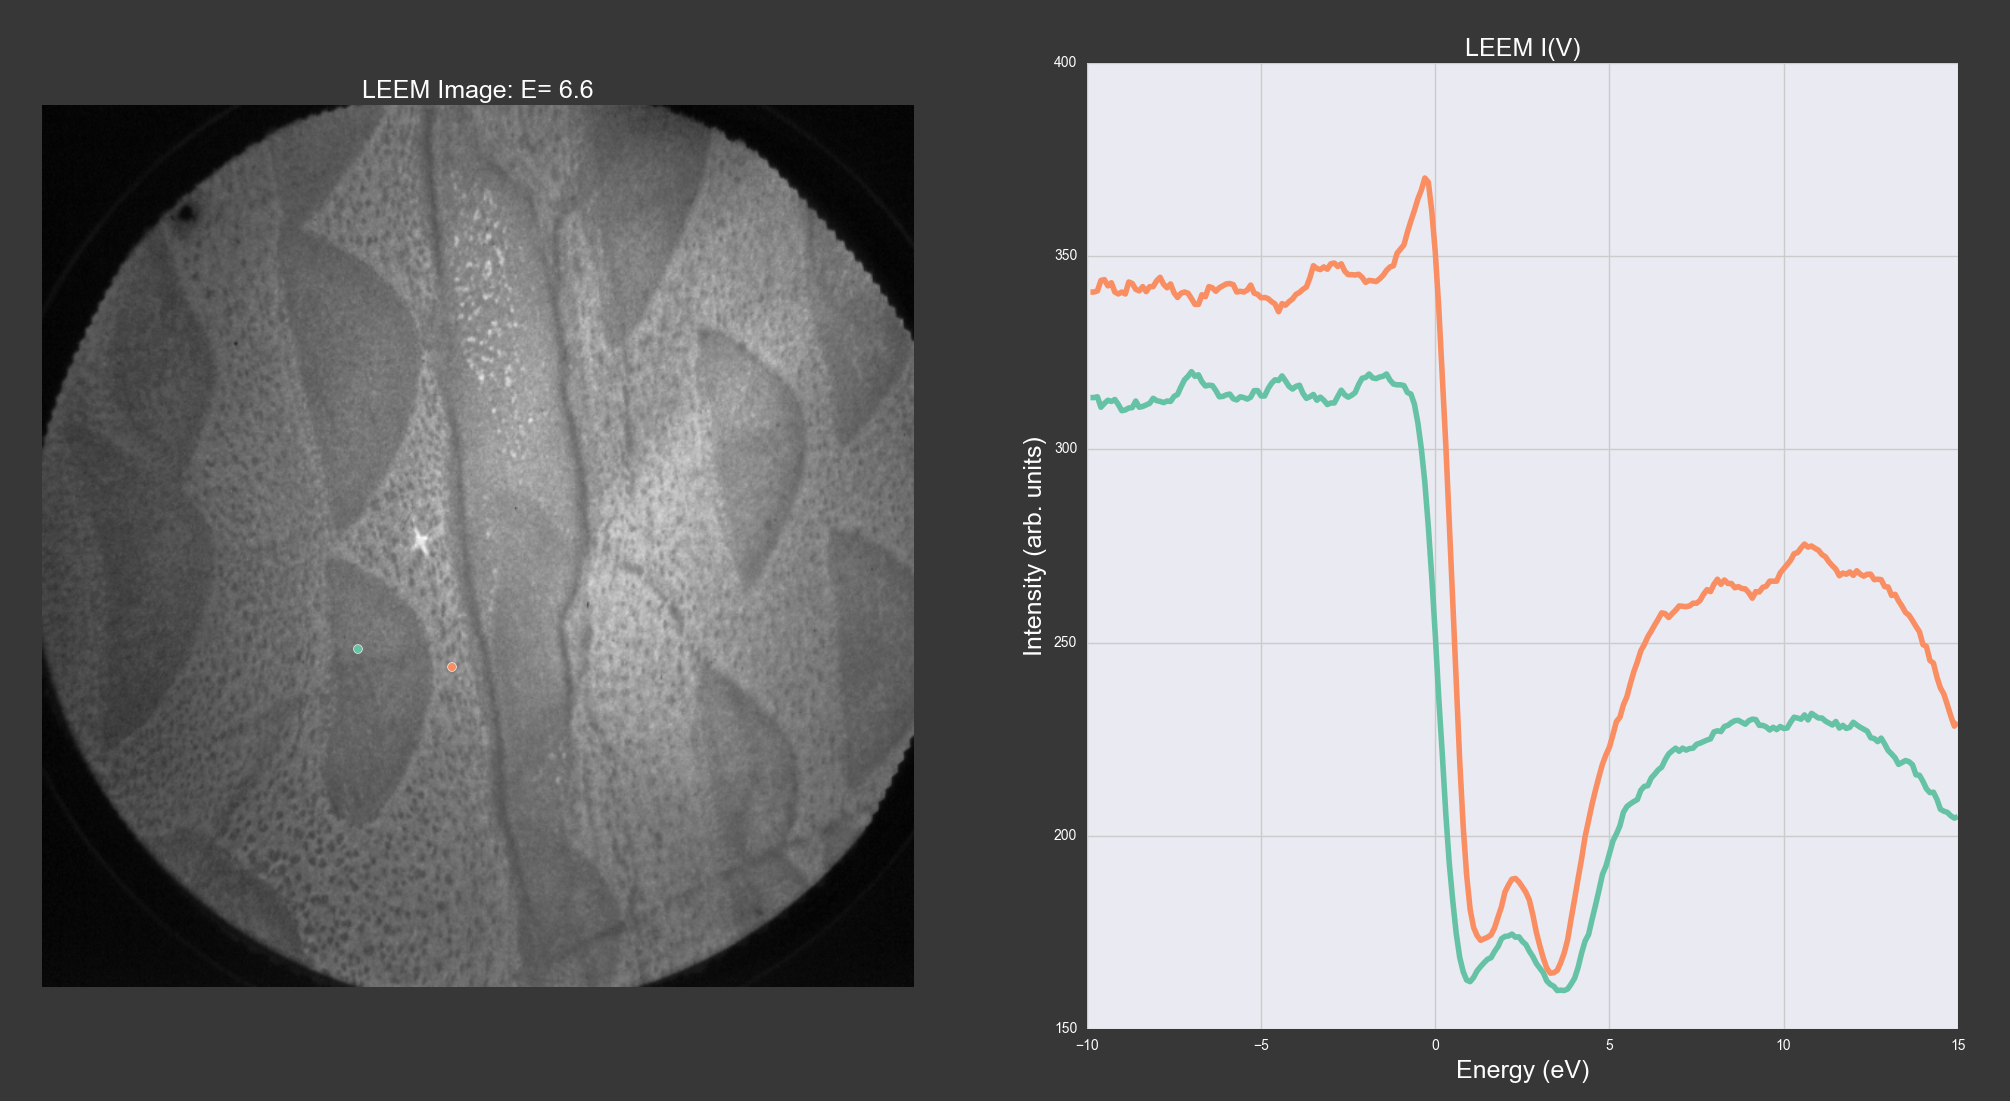
\includegraphics[scale=0.23]{./figs/2dips-2locations.png}
  \caption{LEEM-\textit{I(V)} extracted from two different sample areas displaying similar \textit{I(V)} characteristics. The green curve comes from an area believed to be a graphene island, the orange area would be suspected to be bare ruthenium or ruthenium with amorphous carbon.}
  \label{fig:2dips-2locations}
\end{figure}

Finally, since little STM data was recorded prior to the LEEM investigation of this sample, bilayer graphene can not be fully ruled out as a possibility for the surface structure in this sample. Whereas graphene growth by CVD on ruthenium is a self terminating process resulting in only a single layer, growth by segregation and PVD has the potential to grow multiple layers. Thus, given the inconsistencies present in the LEEM-\textit{I(V)} data extracted from our sample, no definite conclusion can be drawn concerning the sample's carbon layer thickness. However, the data collected during this experiment was still useful. Analysis of the LEEM/LEED images and LEEM-\textit{I(V)} data sets collected laid the groundwork for the PLEASE software package, which is still under active development, and is being used for further studies of numerous 2D materials beyond graphene.

Further data was prohibited as a result of a spark in the electron optics during the third day of analysis. The spark happened near the objective lens, thus the most likely culprit was the sample surface being warped. As mentioned previously, the ruthenium substrate was not uniform and had a pronounced warp/crack on one edge. This part of the sample was then closer to the objective lens than the rest of the sample surface. Given that operation of LEEM requires a very high electric field between the sample surface and objective lens, a rough sample has a tendency to create sparks. After the spark, alignment of the beam became very troublesome.

The final data set collected consisted of a random walk in reciprocal space. The beam alignment made quantitative measurements from the reciprocal space images impossible due to asymmetry in the observed patterns. Walking across the sample and observing the reciprocal space pattern showed mostly LEED signatures from Ruthenium and Graphene. However, one location on the sample was found that contained a very large number of extra diffraction spots in a variety of patterns. The pattern asymmetry makes analysis of the exact periodicity difficult, however, the patterns are still relatively well defined, as shown in Figure \ref{fig:ExtraLEEDSpots}. The cause of these extra peaks can not be confirmed; the spark may have sputtered various metals or other residual gas elements onto the sample surface. The observed patterns do not correspond to the $(2\sqrt{3}$ x $2\sqrt{3})$R30$^\circ$ previously observed via conventional LEED on the polymorphic sample, however, the beam spot size used to acquire this image is more than an order of magnitude smaller than what is possible using conventional LEED at UNH. No definitive conclusions can be drawn from this data concerning evidence of polymorphism.

\begin{figure}
  \centering
  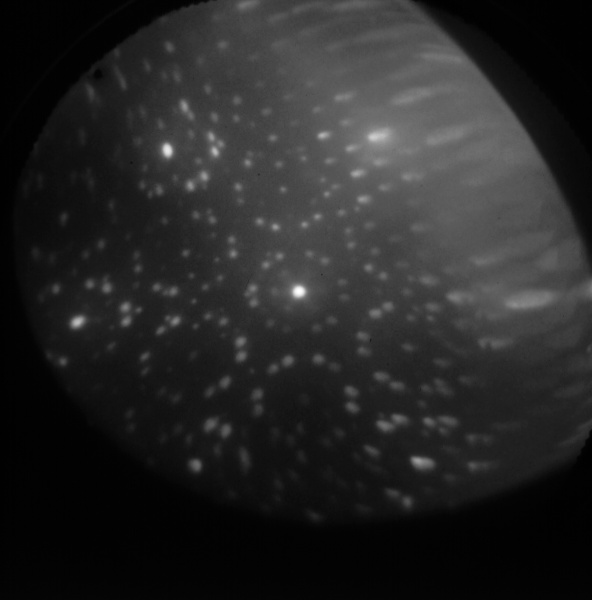
\includegraphics[scale=0.5]{./figs/extraLEED}
  \caption{An area of the sample was observed in reciprocal space which contained many extra diffraction spots relative to the primary ruthenium (1x1) pattern and the carbon moire peaks. Due to beam asymmetry as result of a spark in the electron optics, no quantitative measurements could be performed, nor could a real space image be brought into focus at this point in the sample.}
  \label{fig:ExtraLEEDSpots}
\end{figure}

\section{Results from first LEEM experiment}

Though we were unable to obtain the data concerning the sample surface structure and the carbon layer thickness, the initial experiment was not a total failure. First and foremost, the direct outcome of this experiment was the development of the PLEASE software package for LEEM and LEED data analysis. Chapter 6 will detail further uses of this software with respect to more quantitive analysis of material surface structure. Also, a direct result of this experiment was insight into the difficulties pertaining to data analysis of the polymorphic graphene system's \textit{I(V)} characteristics without a suitable guide for the characteristics for a known structure. To address some of these issues, a second LEEM/LEED experiment focused on furthering our understanding of the growth process was carried out at the Center for Functional Nanomaterials at Brookhaven National Laboratory.


\section{LEEM investigation on the influence of hydrogen in the graphene growth process}
While the first LEEM investigation of polymorphic graphene relied on studying the sample post growth after transit to the LEEM system, our second experiment focused on studying the influence of hydrogen on the growth dynamics of graphene on ruthenium. For this experiment all graphene growth was monitored in real time through LEEM/PEEM. The experiment was carried out at the Center for Functional Nanomaterials at Brookhaven National Laboratory using the Elmitec LEEM-V system, shown in figure \ref{fig:LEEM-V}.

In order to study the effects of hydrogen on the graphene growth process, a source of atomic hydrogen was added to the main LEEM chamber. A commercial thermal gas cracking device provided a flux of atomic hydrogen with controllable pressure to the main LEEM chamber, thus allowing graphene growth to take place in a hydrogen atmosphere while simultaneously imaging the surface with LEEM or PEEM. After installation of the hydrogen cracking source, the LEEM system was baked to obtain low pressures. Next, the electron optics were realigned using a combination of Au/Si and Si(111) samples. Temperatures in the experiment were measured with a C-Type thermocouple attached behind the sample surface. The thermocouple was calibrated using a single point method by observing the silicon (7x7) to (1x1) surface phase transition with real time LEED. The known phase transition temperature of 1100K \cite{Si111} was compared to the TC temp recorded during the transition in order to calculate an offset between the measured temperature and the known temperature. Due to time constraints, only one temperature calibration point was used. Thus the temperatures in this experiment were known to within 25-50K. The difference in LEED pattern observed from the two Si(111) surfaces can be seen in figure \ref{fig:Si(111)}. Future experiments would may more accurately perform the temperature calibration by using a second surface transition at a different temperature to perform a two-point calibration.


\begin{figure}
    \centering
    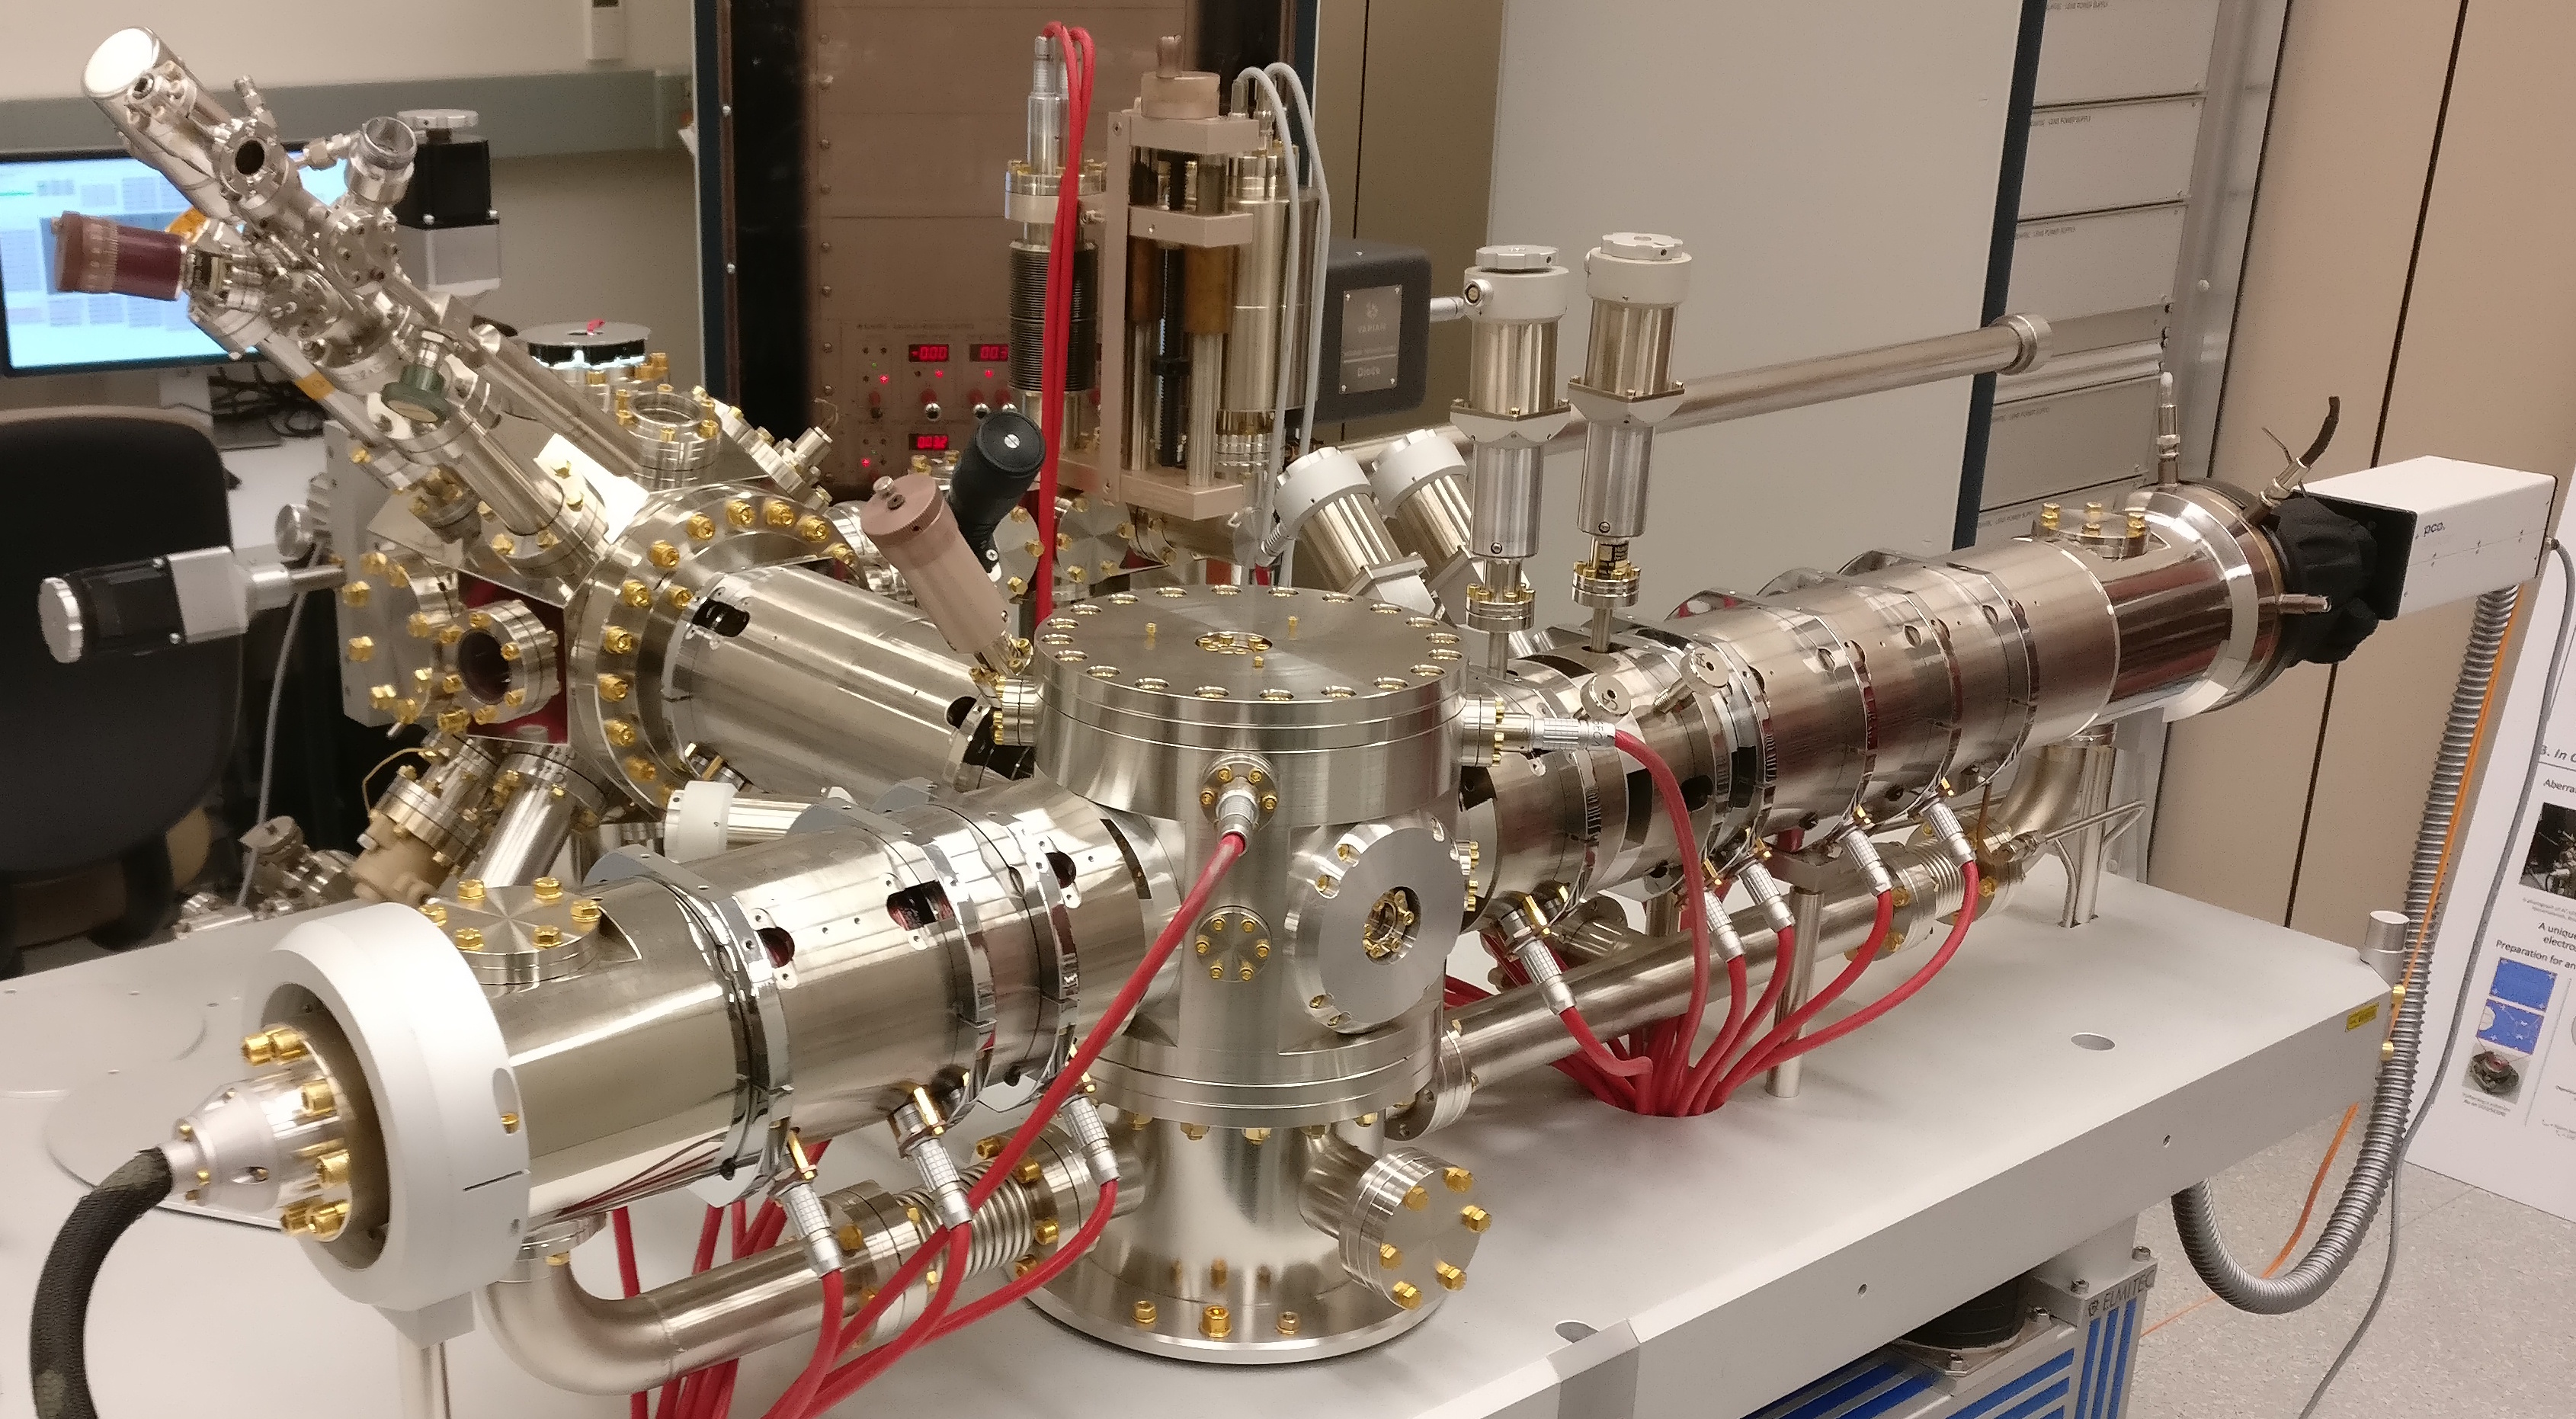
\includegraphics[scale=0.13]{./figs/LEEM-V1.jpg}
    \caption{
    The Elmitec LEEM-V system at the BNL CFN features a T-shape beamline configuration: Electron source (bottom left side); Main chamber, objective lens, and hydrogen cracking source (top left); magnetic prism array (center); imaging column and CCD (right side).
    }
    \label{fig:LEEM-V}
\end{figure}


\begin{figure}
  \subfloat[(7x7) surface reconstruction of Si(111)]{
    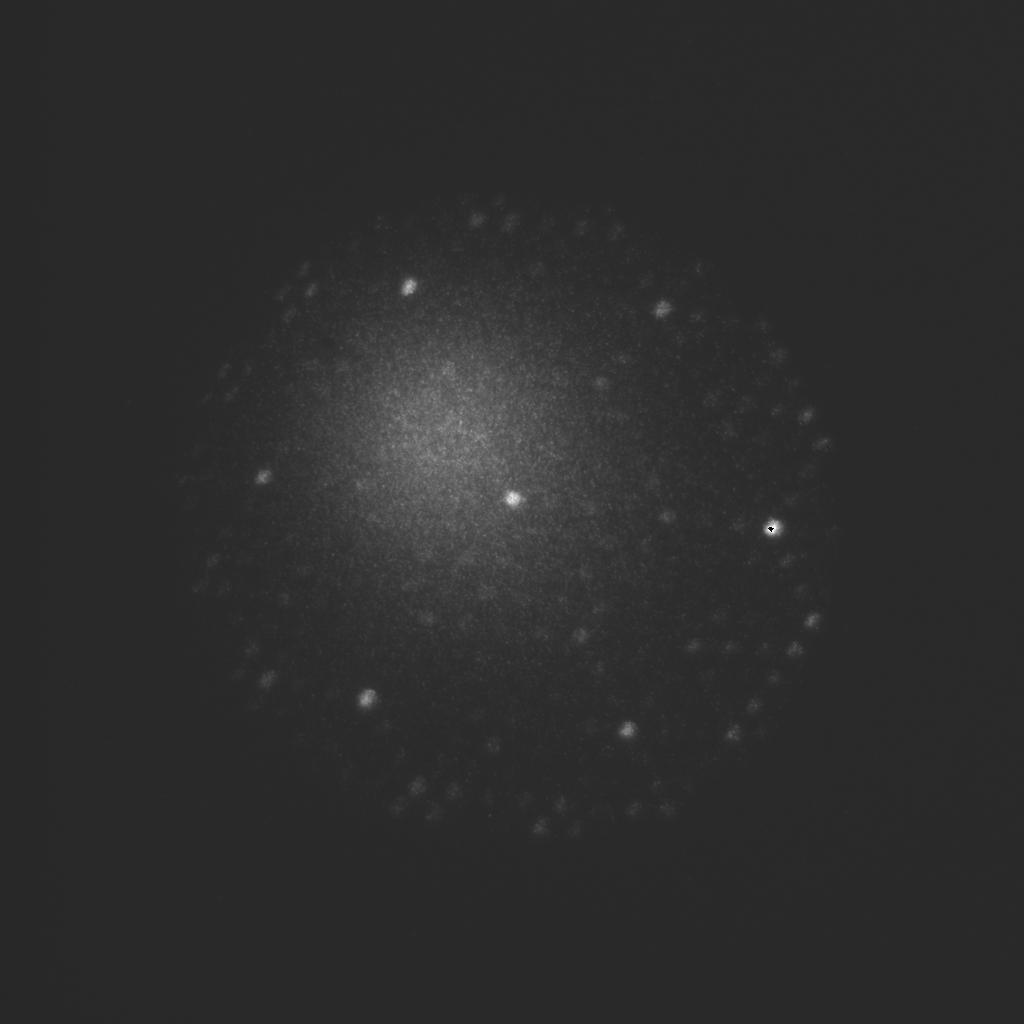
\includegraphics[scale=0.22]{./figs/Si(111)7x7.png}
  }
  \hfill
  \subfloat[Pristine (1x1) Si(111) surface]{
    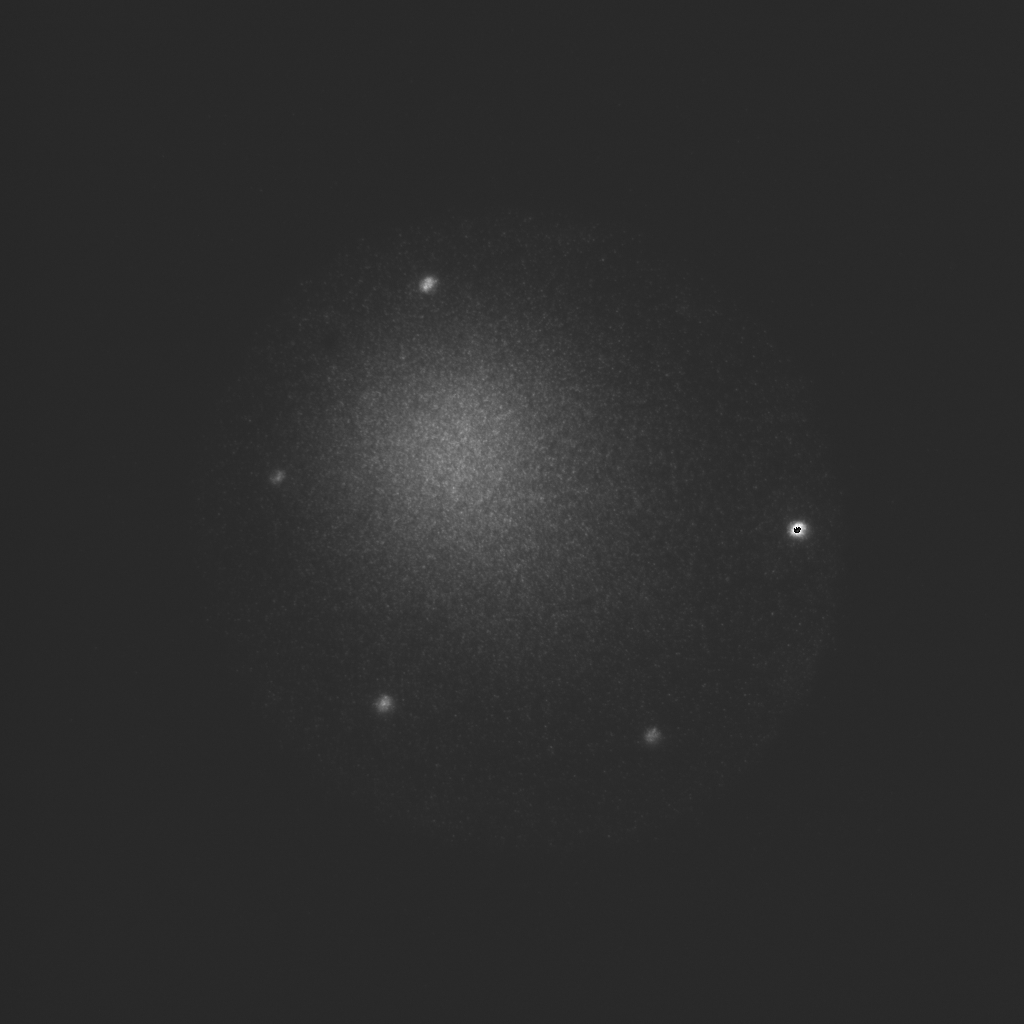
\includegraphics[scale=0.22]{./figs/Si(111)1x1.png}
  }
  \caption{
  The C-type thermocouple was calibrated by imaging the surface of Si(111) in reciprocal space and observing the temperature dependent transition from the (7x7) reconstruction [Left] to the (1x1) phase [Right], which occurs at 1100K.
  }
  \label{fig:Si(111)}
\end{figure}

To begin the sample preparation for this experiment, a Ru(0001) crystal was degassed in the preparation chamber above 400K for a few hours to remove water before being transferred to the main LEEM chamber. Preliminary imaging of the surface showed large amounts of carbon contamination and a high degree of roughness as determined by large amounts of disordered step bunches seen in LEEM. The surface was sputtered with argon ions for 30 mins followed by a standard procedure of exposure to oxygen followed by high temperature annealing to remove carbon. After repeated cycles of oxygen exposure and annealing, a clean Ru(0001) surface was obtained, as verified by a clean Ru p(1x1) LEED pattern free of any other LEED spots as well as a uniformly dark PEEM image. The ruthenium surface has a high work function and thus appears dark when imaged with PEEM, whereas carbon on the ruthenium surface present as adatoms in an amorphous phase or ordered graphene will have a very high signal in PEEM imaging mode.

\begin{figure}
        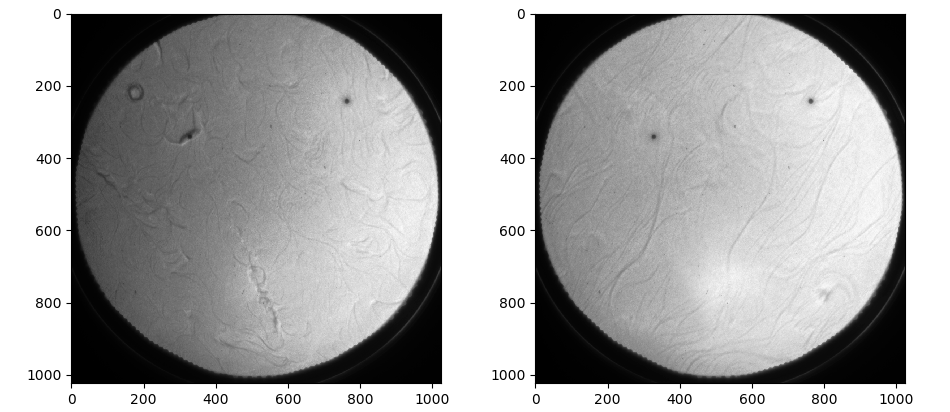
\includegraphics[scale=1.05]{./figs/LEEM-Ru-Before-After-150.png}
    \caption{Real-space LEEM images of the Ru(0001) surface slightly defocused to enhance the contrast of steps and step bunches on the surface. Steps and step bunches appear as dark marks on an otherwise bright surface. Left: 20 micron FOV image of the ruthenium surface after annealing before sputtering. Poor surface quality is indicated by frequency of step bunches and shorter disordered steps. Right: 10 micron FOV LEEM image after sputtering the surface and completing numerous cycles of flash annealing and oxygen exposure. Overall surface quality has improved.
    }
    \label{fig:LEEM-Ru-before-after}
\end{figure}



Figure \ref{fig:LEEM-Ru-before-after} shows two LEEM images of the Ru(0001) acquired before and after sputtering. The image after sputtering appeared clean enough to begin further studies. A LEED-\textit{I(V)} data set was acquired for the clean Ru(0001) surface, covering an energy range of 30-250 eV. A comparison of this data to previously reported conventional LEED-\textit{I(V)} data shows excellent agreement \cite{Ru-LEED-old}. While previous studies on the ruthenium surface structure utilized conventional LEED, our study acquired LEED data via LEEM. Thus, included in our data is the \textit{I(V)} curve for the (0,0) spectrally reflected beam, which is typically absent from conventional LEED experiments unless an off-normal angle of incidence is used. Thus, it may be worth analyzing the optimized surface structure obtained by fitting this data to dynamic electron multiple scattering models.

After analyzing the pristine ruthenium surface, the temperature parameters for graphene growth via bulk segregation were determined. The sample surface was doped with a small amount carbon via catalytic decomposition of ethylene using a CVD process. At high temperature, the $C_{2}H_{4}$ adsorbate molecules decompose into carbon adatoms and free hydrogen molecules. This process is easily visualized in real-time with PEEM due to the large difference in work function between ruthenium and carbon. Carbon adatoms and ordered graphene islands appear as bright areas atop a dark ruthenium background. Utilizing the fact that the carbon solubility in ruthenium changes as a function of temperature, the surface phase carbon was adsorbed into the bulk ruthenium crystal at a temperature above 1000$^\circ$ C which agrees with previous results \cite{mccarty-carbon}. At this point the PEEM image of the surface returned to a uniformly dark image devoid of structure indicating the surface was only ruthenium and was ready for graphene growth via segregation. Slowly cooling the sample from 1000$^\circ$ C while recording the PEEM image every few seconds provided a movie of the graphene growth process. As the ruthenium temperature cooled, the bulk carbon solubility dropped and thus the interstitial carbon atoms diffused to the surface. The initial nucleation of carbon surface atoms appeared as a small bright spot atop the dark ruthenium background. Growth continued slowly outward from the initial nucleation point in a somewhat dendritic fashion, indicating relatively poor surface quality.

Figure \ref{fig:seg-growth} shows a sequence of images from the bulk segregation growth process described above. The initial image shows a uniformly dark ruthenium surface devoid of any photoemission signal from the light source used. As the temperature of the crystal cools from temperatures above 1200 K, carbon begins to segregate from bulk to surface. This can be seen as bright spots that appear in the later images. The islands grow outwards from the initial nucleation points. The rate of growth is influenced by a number of factors such as temperature and relative bulk carbon abundance. The kinetics of the growth process are explained in detail by McCarty et al \cite{mccarty-carbon}. Depending on the initial amount of available carbon from CVD doping and the growth time, graphene islands could be grown up to tens of microns in size.

The process of growing graphene via segregation is a reversible process. After growing islands, the sample can be heated again to high temperatures (T $>$ 1600 K) to dissolve the carbon back into the crystal bulk. This was repeated numerous times to get a better understanding of the heating and cooling parameters required to grow repeatedly grow pristine graphene islands. Next, the influence of atomic hydrogen on as-grown graphene was studied. The process of CVD doping, dissolving of surface carbon, and finally growth by segregation was repeated to nucleate a large graphene island with a length dimension larger than 20 micron.

After the island was grown, it was exposed to a flux of atomic hydrogen and monitored with LEEM to look for changes in the local electron reflectivity or other signs of interaction with the hydrogen. The idea behind this study was that it may be possible for the hydrogen to intercalate at the graphene-ruthenium interface, thus lifting the carbon layer higher above the ruthenium and passivating the ruthenium surface. While monitoring the LEEM signal from the graphene surface during hydrogen exposure at a pressure of 1 x 10$^-6$ torr, little change was observed. The sample was then subject to prolonged annealing in a hydrogen atmosphere. The only difference observed over time was mild etching of the graphene island edges. Without a simultaneous residual gas analysis of the reaction, it is difficult to determine the specifics of the observed reaction. One possibility is a reaction between hydrogen (as molecular gas phase or in atomic phase) and the graphene island edge, producing a hydrocarbon of the form \ce{C_{x}H_{y}}. Another possibility is the reaction between oxygen impurities in the hydrogen atmosphere and the graphene island edge. Oxygen is known to react with carbon at the ruthenium surface to create \ce{CO} and \ce{CO_{2}} molecules. This is the primary method for cleaning a ruthenium surface to remove unwanted carbon contaminants. A previous study has shown that oxygen contamination can induce graphene etching in graphene grown by CVD on copper foils, and furthermore, this etching can be minimized or halted altogether by using ultra purified hydrogen \cite{graphene-etching}. A second study indicates that the reaction for oxygen etching on ruthenium proceeds with a relatively low activation energy \cite{graphene-etching-ru-O2}

Regardless of what chemical reaction is involved in the graphene etching process, it was noted that during a prolonged annealing in a hydrogen atmosphere, the etching process did not continue to the entirety of the graphene island. Actually, very little surface area of the island was etched away. One possible explanation of this could be a reaction terminated by ruthenium step edges.  Graphene on ruthenium tends to grow in a ``carpet-like'' fashion, where the graphene islands grow preferentially in a the downhill direction on the ruthenium terraces with little to no growth in the uphill direction. Similarly, the etching process via hydrogen atoms or other gas impurities may etch the island up to the nearest step edge in the uphill direction and then terminate. The carbon atoms at the step edge may be more strongly bound to the ruthenium surface as a result of the higher coordination number for ruthenium atoms at the step edge. This stronger binding may interrupt the etching process.

To summarize the findings for the interaction of hydrogen with as-grown graphene islands: no signs of intercalation were observed via PEEM, LEEM, and LEED. The LEED patterns observed from graphene before and after addition of the hydrogen remained unchanged indicating no structural changes in the graphene overlayer, and the LEEM images showed no observable change in electron reflectivity. To continue the experiment, we then analyzed the effects of graphene growth on ruthenium in a hydrogen atmosphere rather than observing the effect of hydrogen on an already grown graphene island.


\begin{figure}
  \subfloat[t = 0s]{
    
\includegraphics[scale=0.22]{./figs/PEEM-73.png}
  }
  \hfill
  \subfloat[t = 10s]{
    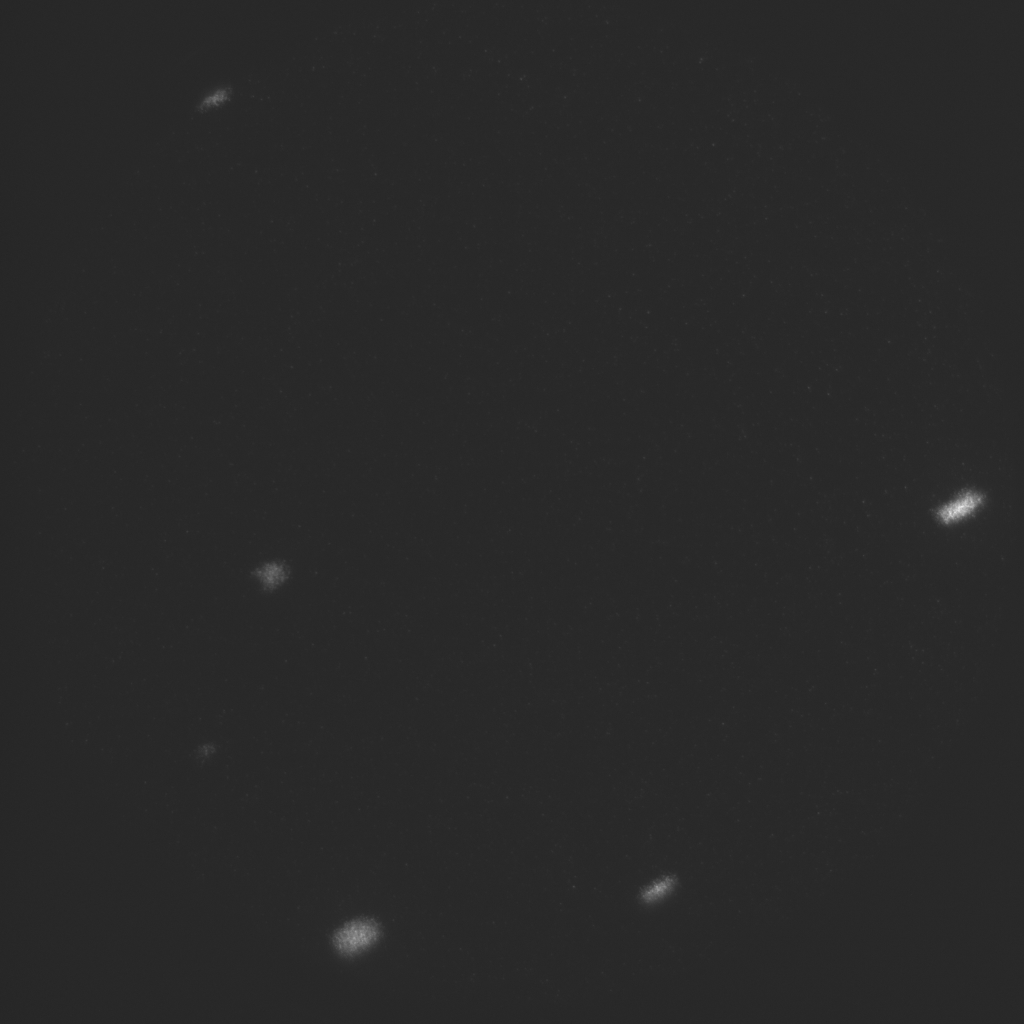
\includegraphics[scale=0.22]{./figs/PEEM-75.png}
  }
  \\
  \subfloat[t = 60s]{
    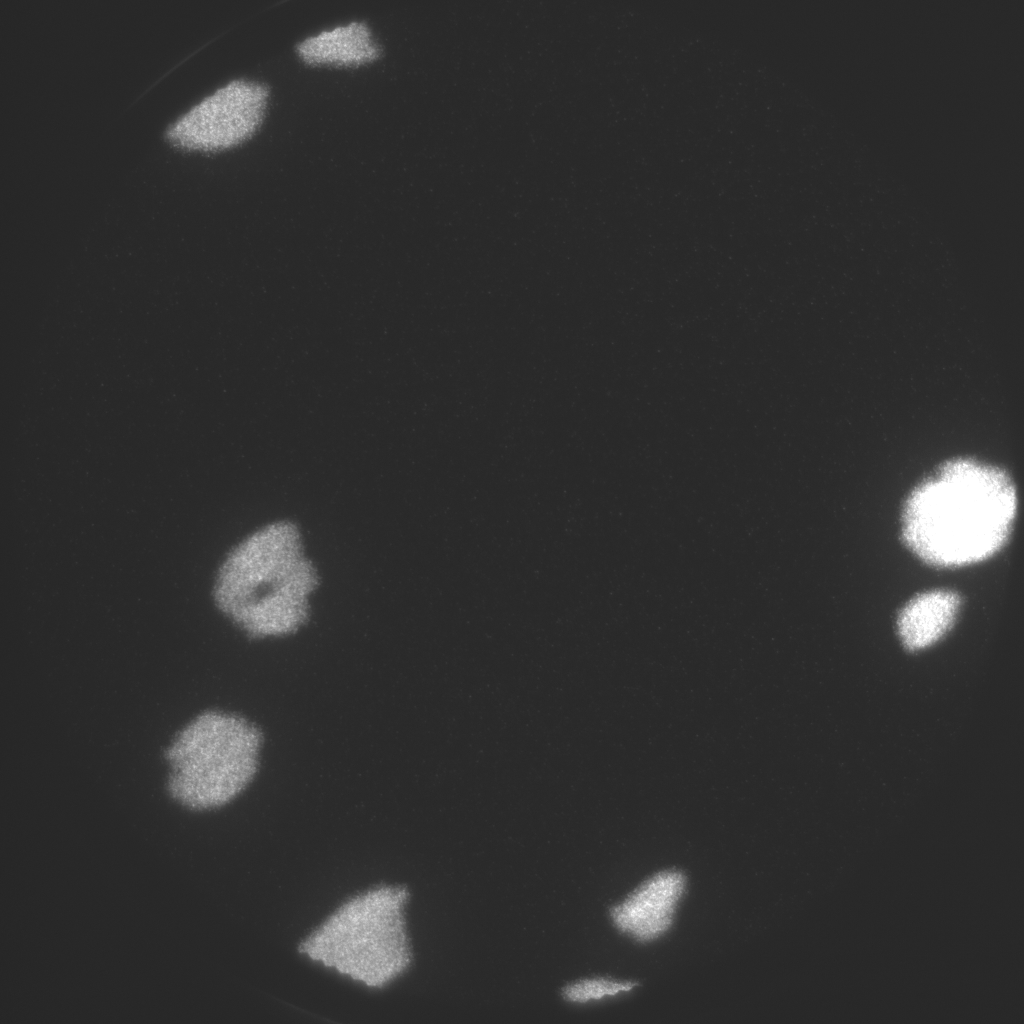
\includegraphics[scale=0.22]{./figs/PEEM-85.png}
  }
  \hfill
  \subfloat[t = 120s]{
    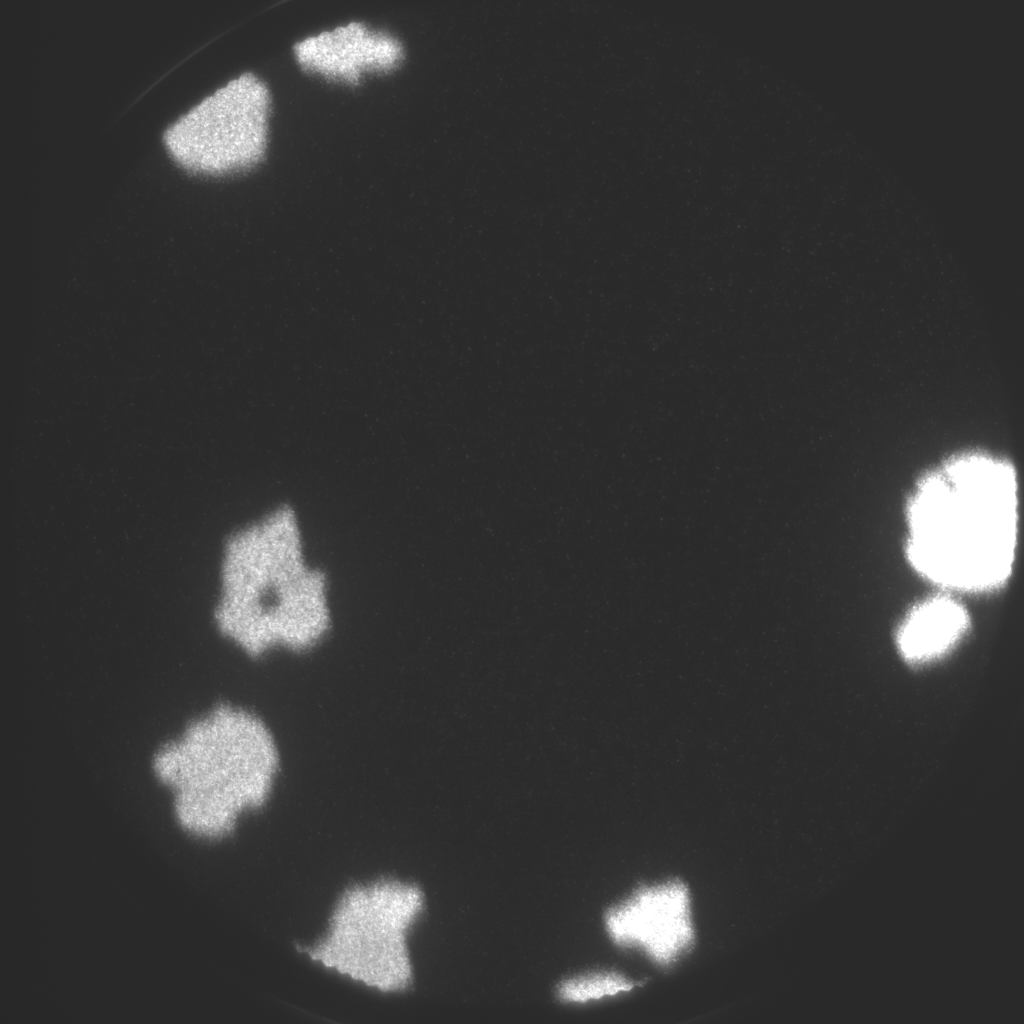
\includegraphics[scale=0.22]{./figs/PEEM-104.png}
  }
  \caption{Time sequence of PEEM images detailing growth of graphene islands via bulk segregation of interstitial carbon atoms from a Ru(0001) crystal. Field of View in all images is 30 micron; all times are approximate to within a few seconds, and the growth temperature is approximately 1075 K. The dark background is the ruthenium surface, devoid of any photoemission signal, as shown in panel a. The bright spots in later images indicate carbon islands that grow outward from the initial nucleation points shown in panel b.
  }
  \label{fig:seg-growth}
  \end{figure}

 To study the effect of hydrogen on the growth process of graphene on ruthenium, first the sample was pre-doped with carbon via CVD of ethylene at high temperature. Next, the surface carbon was adsorbed into bulk by high temperature annealing. The process was monitored in real time via PEEM. When the PEEM surface image became nearly uniformly dark, indicating no surface carbon. Finally, before regrowing graphene, the LEEM main chamber was backfilled with atomic hydrogen at a pressure of $10^{-6}$ torr. The process of carbon adsorption into bulk was then reversed by slowly cooling the sample from above 1000 $^\circ$ C. The growth of graphene islands via bulk segregation in a hydrogen atmosphere was monitored with LEEM and the process was continued until multiple large area islands had nucleated. Figure \ref{fig:three-islands} shows a 30 micron FOV image of three graphene islands after growth in a hydrogen atmosphere. Using the LEEM control software, three areas in the island centers were marked for analysis with LEED.

 Next the LEED patterns acquired from each island were observed by placing a 5 micron beam limiting aperture inline with the reflected/diffracted beam signals in the imaging column of the microscope and then aligning the data acquisition area with one of the previously marked locations. At each island, LEED-\textit{I(V)} data was also collected. Neither island displayed different characteristics in the observed LEED pattern compared to that of graphene grown via segregation without hydrogen. The $2\sqrt{3}$ x $2\sqrt{3}$R30$^\circ$ pattern observed after growth of polymorphic graphene at UNH was not observed after any combination of during-growth or post-growth hydrogen exposure. One possible explanation of the lack of signal of hydrogen interaction could be that the distance between hydrogen cracking device and the sample/objective lens system was too large. Given that the cracking device had to be integrated with the main LEEM chamber to to real time monitoring of the growth process, the distance to the hydrogen cracker could not be adjusted. If the mean free path of the atomic hydrogen atoms was too short, then a sufficient flux of atomic hydrogen would not reach the surface before recombination. A partial solution to this issue will be addressed later as a future experiment.

 Graphene samples were prepared using a variety of growth techniques. the CVD growth process using ethylene was the quickest way to achieve essentially a full monolayer of graphene due to the catalytic decomposition process being self terminating. However, the graphene grown by CVD was generally of poor quality, which could be seen in two ways. First, by monitoring the growth in real time it was observed that the CVD growth process proceeded from a very large number of nucleation points. Graphene would grown outward from each nucleation point resulting in a very large number of small graphene islands. As the monolayer grew to completion, the small graphene islands grew and merged together, however the domain boundaries between the individual islands did not fully go away. When observing the LEED pattern from CVD graphene it was evident that there was a very large degree of rotational disorder, likely resulting from the domain edges. It may be possible to recover a better LEED signature by a prolonged annealing of the CVD graphene sample, however this was not tested.

Graphene grown via bulk segregation generally resulted in higher quality graphene samples as characterized by LEED, however this comes with a number of downsides. The process of growth by segregation is very dependent on the initial conditions of carbon concentration in the bulk and near surface region of the ruthenium crystal. Growth will only continue while there is sufficient diffusion of interstitial carbon atoms through the bulk to the surface, thus the size of the graphene layer grown is limited by the carbon concentration. In contrast to the CVD growth process, bulk segregation is not a self terminating growth process. If there is sufficient carbon concentration in the bulk region, then multiple graphene layers can be grown. The second layer will not begin to grown until the surface has achieved approximately 0.80ML coverage, and will grow from below the first layer. \cite{sutterleem, Graphene-on-metals}

 \begin{figure}
     \centering
     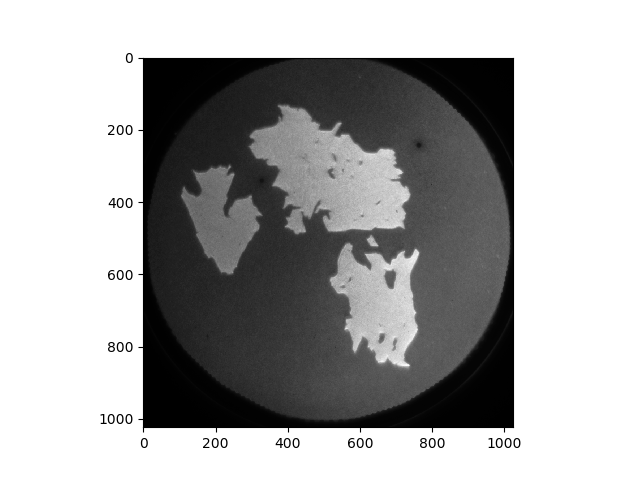
\includegraphics[scale=1.1]{./figs/LEEM-three-islands-with-H.png}
     \caption{30 micron FOV displaying three large area graphene islands grown via bulk segregation of carbon in a hydrogen atmosphere. To look for indications of structural changes resulting from hydrogen interaction, each island was examined using LEED.
     }
     \label{fig:three-islands}
\end{figure}

After analyzing the growth of graphene on ruthenium under a hydrogen atmosphere using a variety of growth parameters, no LEED signatures of hydrogen influence were observed. This prevented further analysis of the surface structure parameters via LEED-\textit{I(V)} of the polymorphic graphene system. However, a number of brightfield LEEM-\textit{I(V)} data sets were collected to analyze the carbon layer thickness in the sample. First, the sample was cleaned using the previously mentioned method of cycles of high temperature annealing and oxygen exposure. Once the ruthenium surface was deemed essentially free of carbon by analyzing PEEM images and the $\mu$-LEED pattern, a brightfield LEEM-\textit{I(V)} data set was acquired for the pristine Ru(0001) surface.

Next, graphene was grown via bulk segregation in a hydrogen atmosphere until large single layer islands had nucleated. Analysis of the sample surface with LEEM showed numerous large scale single layer graphene islands with uniform electron reflectivity contrast. The total coverage of the surface at this point was estimated to be near 0.6-0.7 ML. A second LEEM-\textit{I(V)} data set was acquired for a large area single layer graphene island. Finally, the single layer graphene sample was subjected to a prolonged annealing in the 700-900 $^\circ$ C range causing additional carbon to segregate from the bulk to the surface region. The process was monitored with brightfield LEEM with an electron energy near 3.5 eV. during this process, the surface area between visible islands became noticeably lighter in contrast, indicating an influx of carbon adatoms. Before the surface was fully covered with a monolayer of graphene it was noted that certain areas of the single layer graphene island began to change contrast in the electron reflectivity signal. Areas of the single layer graphene island nucleated with a darker contrast compared to the surrounding area, and slowly grew over time during the annealing process. When the dark contrast areas on the graphene island had grown to a sufficient size, the annealing process was halted and a third and final \textit{I(V)} data set was collected.

Using the PLEASE software package, the LEEM-\textit{I(V)} data sets were analyzed to examine differences in the shape of the very low energy regime of the \textit{I(V)} curves. First a region of the clean ruthenium (0001) surface was used for \textit{I(V)} extraction. By analyzing the LEEM images in the mirror electron energy range, the greatest contrast is found between ruthenium terraces and atomic steps or step bunches. Care was taken to extract \textit{I(V)} data from a region with minimal steps and step bunches to improve the data quality. For the second data set, three areas of the single layer graphene island were chosen. The images from the mirror electron energy range again provided the greatest contrast between the graphene island surface and defects or impurities present. The three regions were chosen such that there were minimal defects included. Finally


Finally, areas of the single layer graphene island and areas in the darker regions within the islands were used for data extraction. Distinct differences are observed between each \textit{I(V)} curve, as shown in Fig. \ref{fig:LayerThickness}. This difference can be attributed to the samples containing different thickness of carbon at the surface region. The dark regions formed after annealing single layer graphene indicate areas of the sample that contain bilayer graphene. This layer grows from below the surface as carbon segregates upwards from the bulk \cite{Graphene-on-metals}.

\begin{figure}
\centering
  \subfloat[Clean Ru(0001)]{
    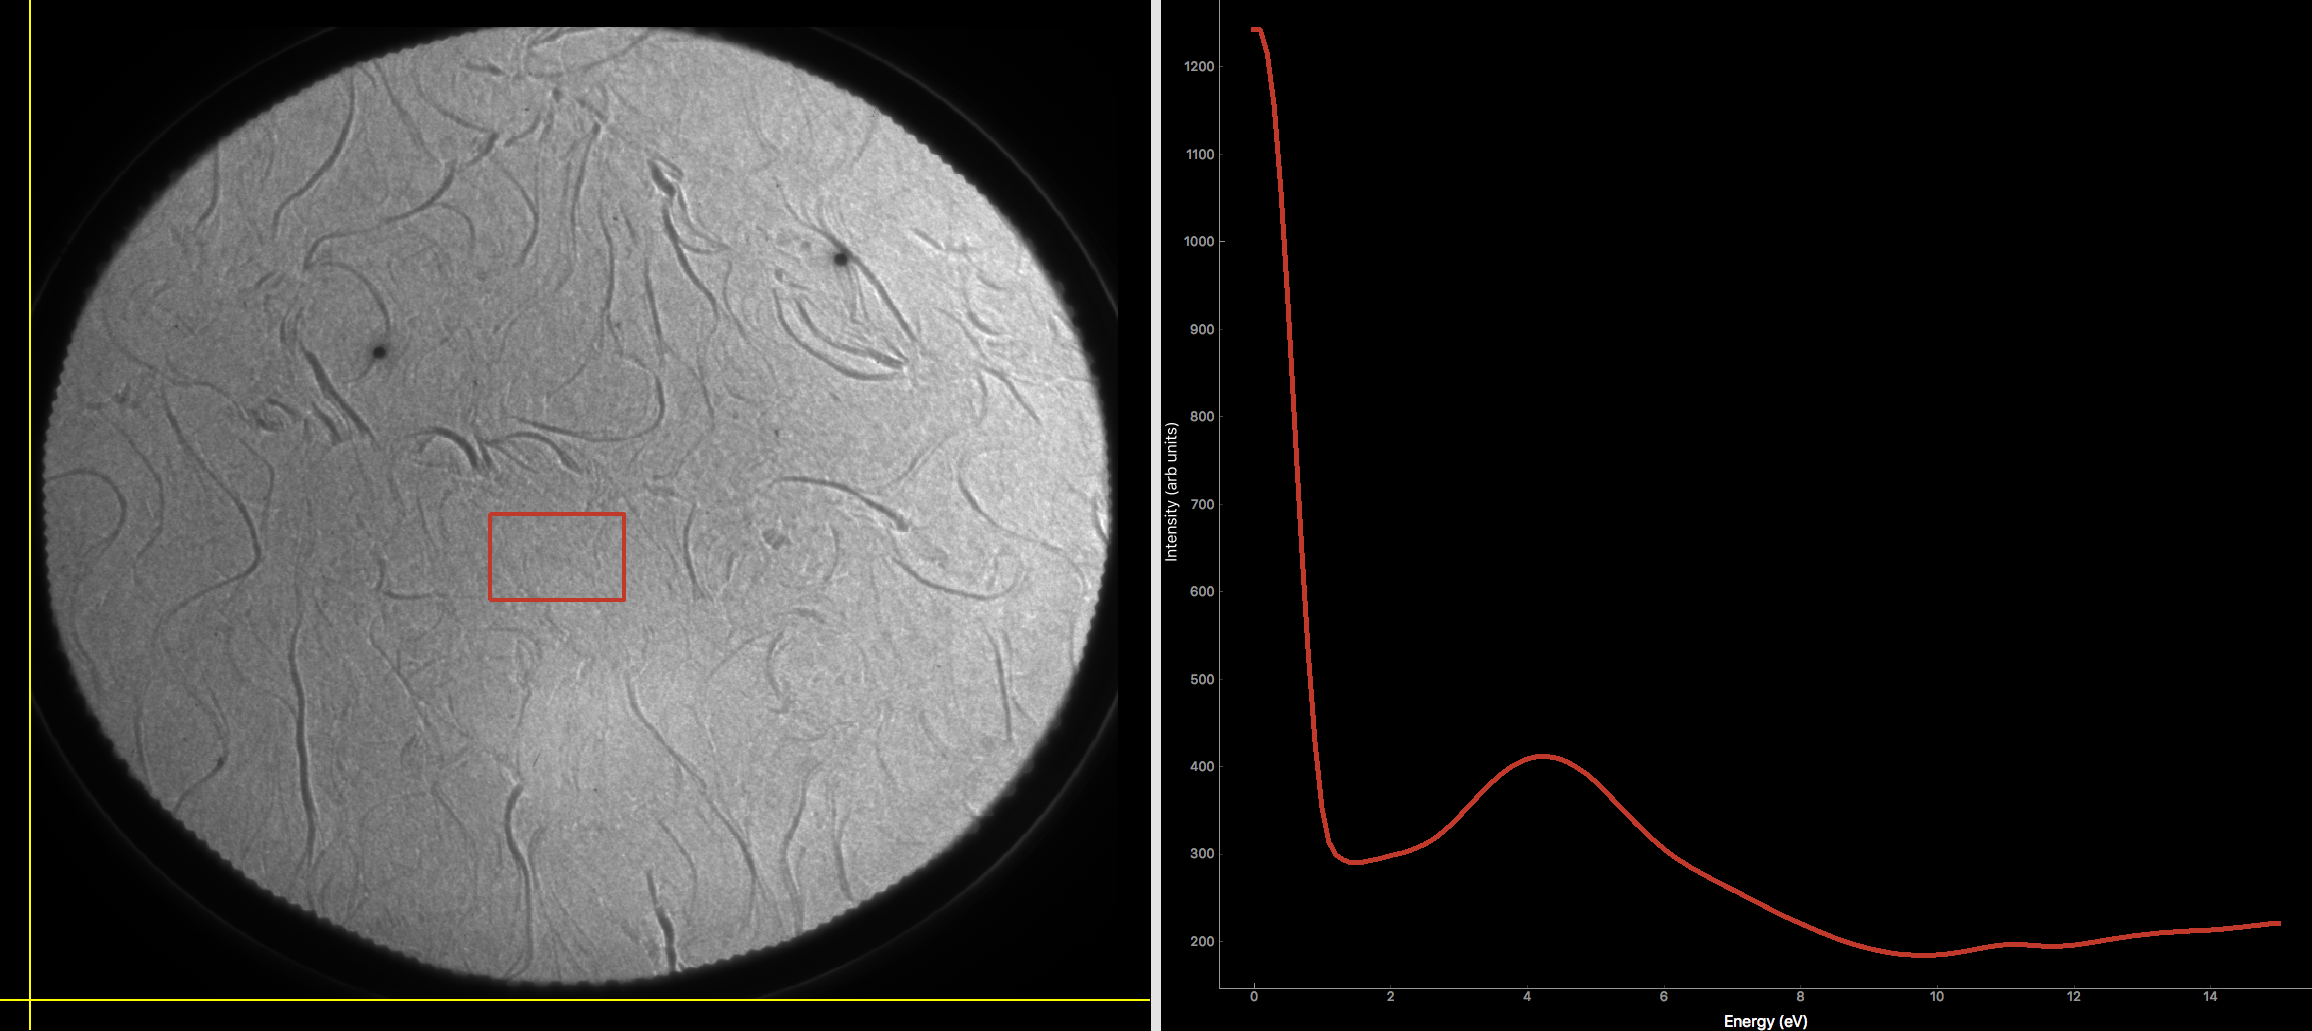
\includegraphics[scale=0.15]{./figs/Clean-Ru(0001)-LEEM-IV-2}
  }

  \subfloat[SlG/Ru(0001)]{
    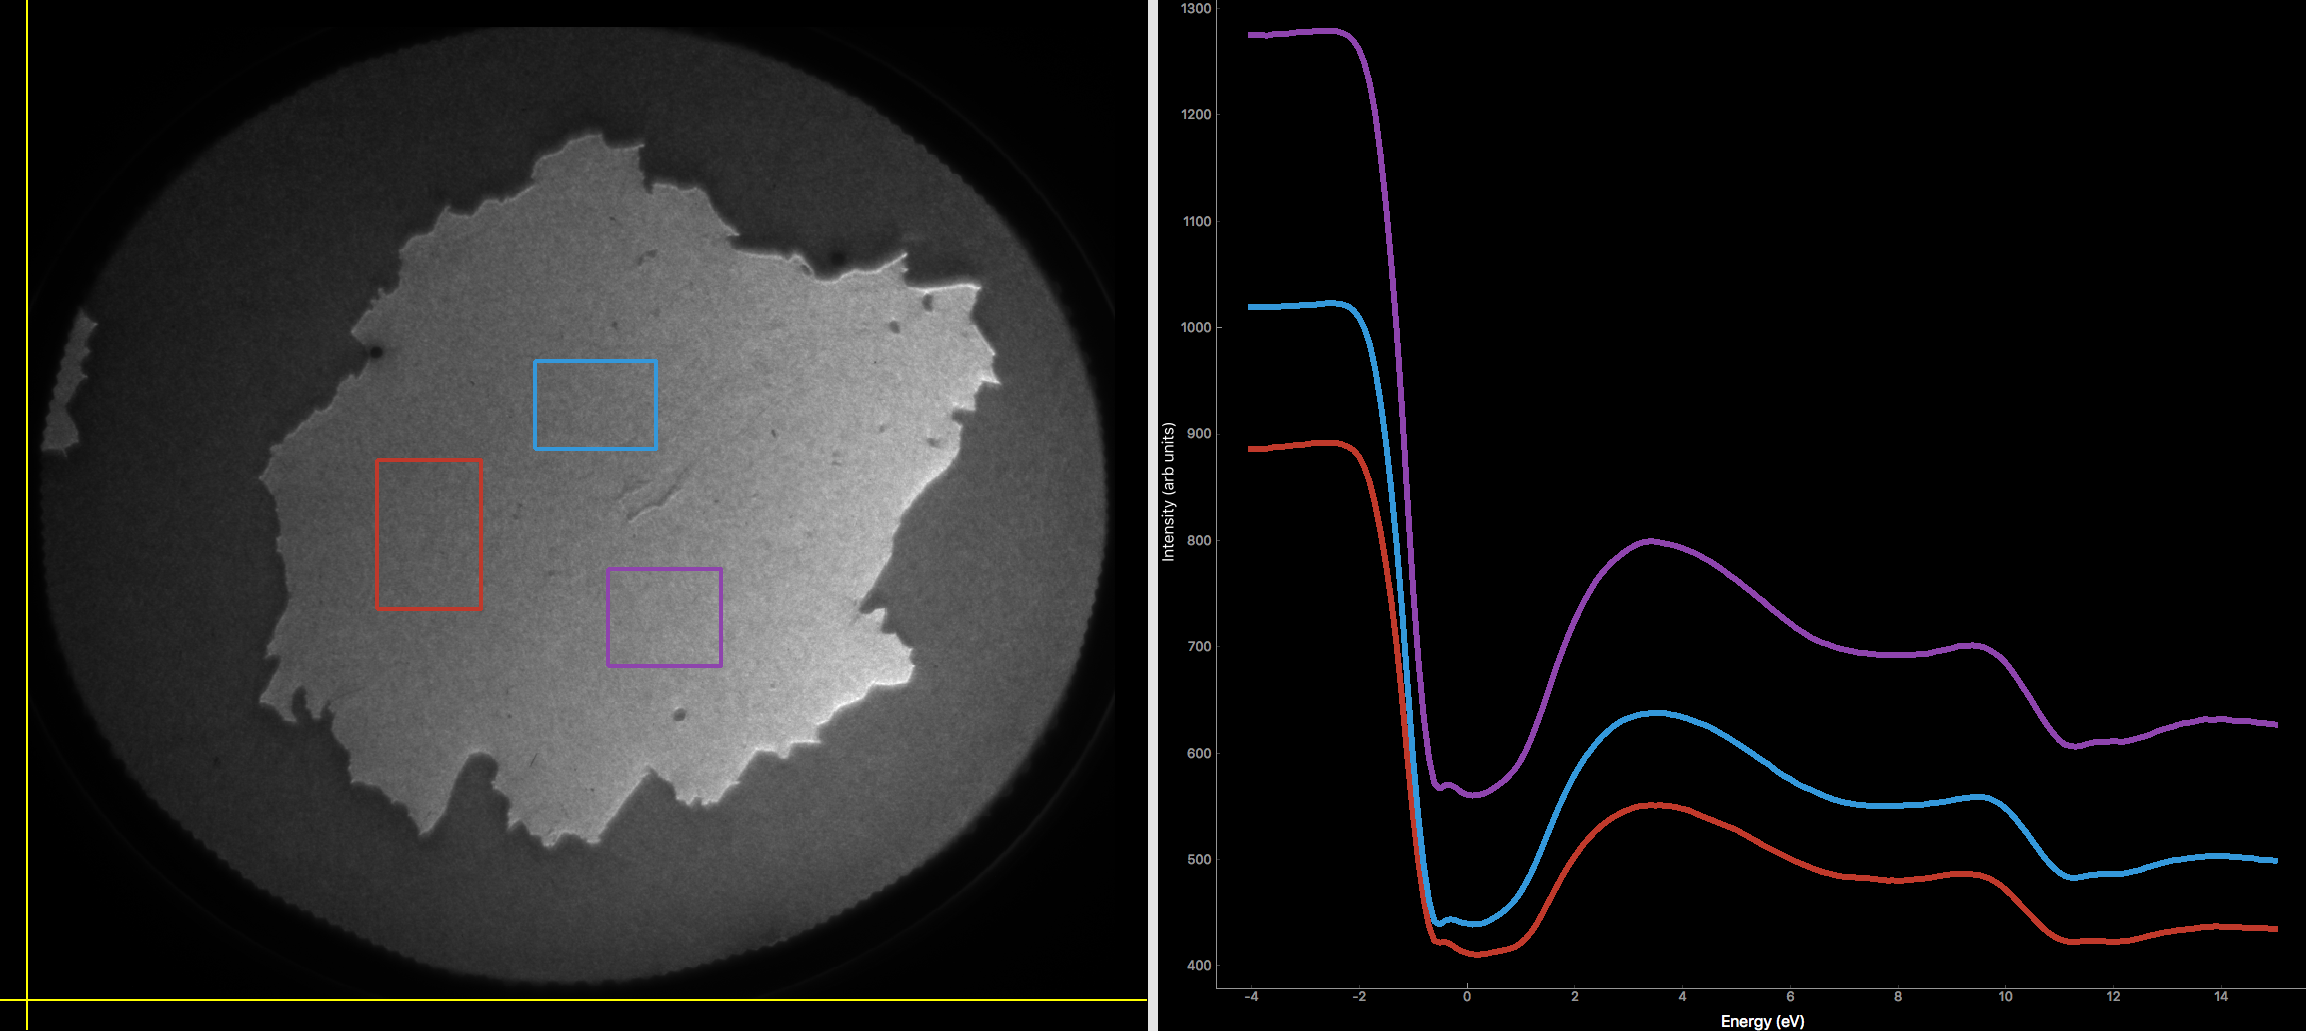
\includegraphics[scale=0.15]{./figs/SLG-LEEM-IV-2}
  }

  \subfloat[BLG/Ru(0001)]{
    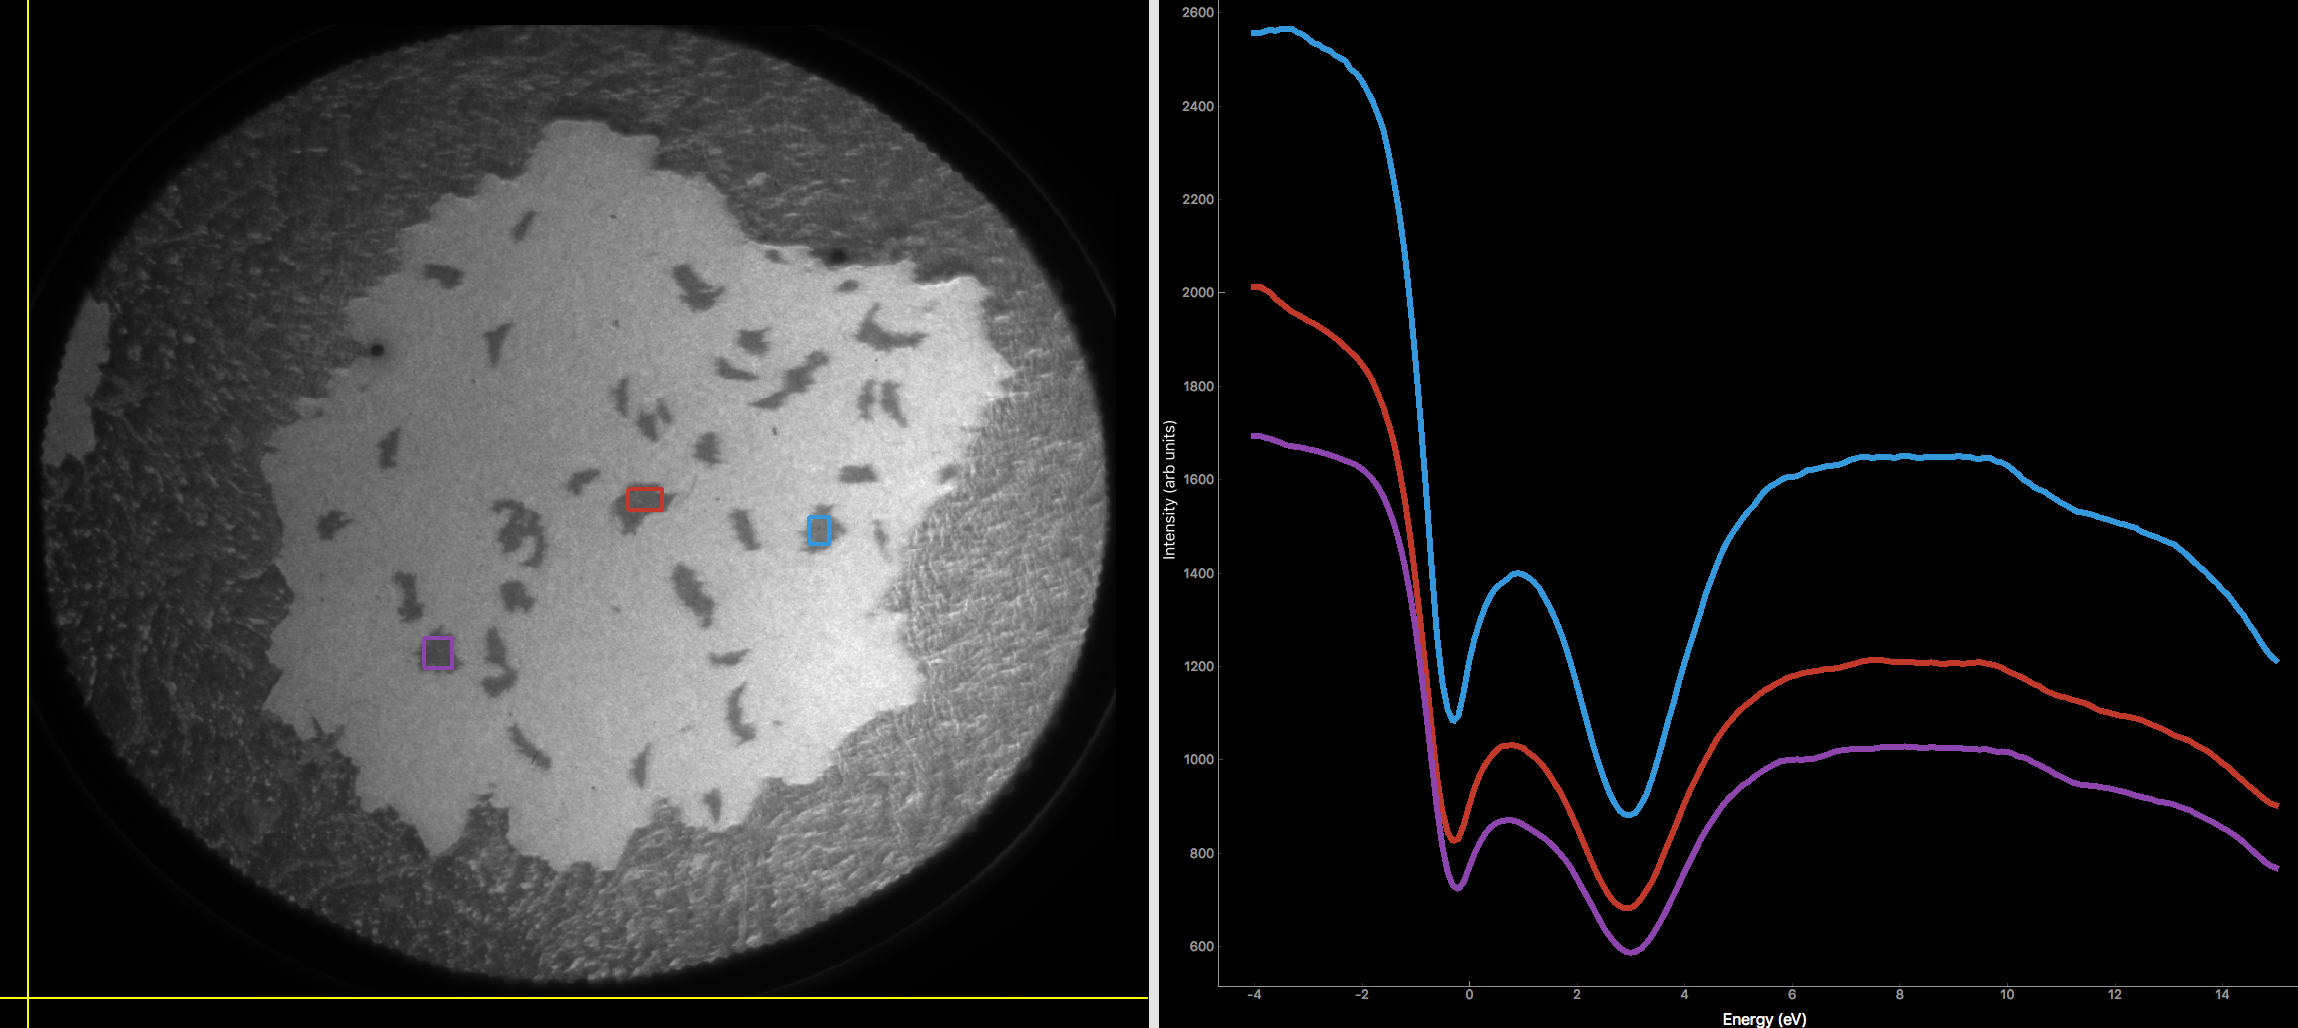
\includegraphics[scale=0.15]{./figs/BLG-LEEM-IV-2}
  }
  \caption{Brightfield LEEM-\textit{I(V)} showing distinct features for three separate surfaces. This demonstrates the capabilities for using LEEM-\textit{I(V)} as a method to characterize the layer thickness in layered materials and thin films.
  }
  \label{fig:LayerThickness}
\end{figure}

% Chapter Name
\chapter{\sc Novel Layered Materials Studied with LEEM/LEED-I(V)}
\label{ch:Novel Layered Materials Studied with LEEM/LEED-I(V)}

The study of the fundamental properties of materials and their applications has long been the driving factor in major technological advancements. Applications of novel materials are abundant in areas of research such as sustainable energy sources, healthcare technology, energy efficient transportation, and high speed computing devices \cite{novel-materials}. While not all problems faced by modern society will have a technological solution, it is safe to say that research and innovation in materials science will be crucial to the development and adaptation of many answers to these challenges.

The ability to manipulate and grow materials at the nanoscale has already enabled development of numerous technological advances based on nanotechnology. A wide range of applications from medicine to electronics have been demonstrated using nanoscale materials \cite{nanocancer, energystoragematerials}. The discovery of graphene demonstrated that carbon can be used for nanoscale devices in solid form ranging from zero to three dimensions and furthermore proved that the two-dimensional solid form was not prohibited. However, this discovery also lead to an explosion of research into other materials beyond graphene, which are also stable in two-dimensional form. Given that many new materials have been discovered to be stable in single layer or two-dimensional form, it should be expected that in the future nanotechnology will encompass a wide variety of materials beyond carbon \cite{2d-atlas}.

Many of the currently explored 2D materials posses unique layer dependent electronic properties \cite{2D-TMDs}. Furthermore, single layer and 2D materials span the configuration space of electronic structure from traditional metals, semiconductors, and insulators to more exotic types of materials such as Weyl semimetals, topological insulators, and novel magnetic materials \cite{2d-atlas}. Thus it may be possible in the future to harness the properties of many 2D materials and combine them into devices based on layered heterostructures.

Before devices and new technology can be generated from novel 2D materials, the material properties must be studied at the atomic scale. While many characterization techniques are useful for providing three dimensional structural information for bulk phase materials, the study of the structure of materials in 2D form requires highly surface sensitive probes. Furthermore, given that many current 2D materials are exfoliated into small flakes as opposed to grown via MBE, their characterization requires a probe that can be localized to the micrometer scale and below while also remaining non-destructive. This combination of requirements dramatically reduces the number of possible tools suited for the task.

Here I present a brief overview of the study of two-dimensional materials using LEEM and $\mu$-LEED to analyze the surface structure with {\aa}ngstr\"{o}m level precision. My initial work developing software to analyze LEEM data from our experiments on polymorphic graphene proved immensely useful in a more general sense to analyze both LEEM and LEED \textit{I(V)} data sets from a wide array of surface science experiments concerning the surface structure determination of 2D materials. More information on these studies including their experimental setup as well as corresponding computational and theoretical work can be found in their associated publications as well as the thesis work of my colleague, Zhongwei Dai.


\section{Molybdenum Disulfide}

Molybdenum disulfide belongs to a class of materials known as transition metal dichalcogenides (TMDs). These materials have the formula MX$_2$ where M is a transition metal cation and X is a chalcogen anion; chalcogen atoms fall under group 16 in the periodic table of elements. The molybdenum disulfide bulk crystal structure is composed of sets of layers three atoms in thickness whereby a molybdenum atom is sandwiched between two sulfur atoms. These individual three atom layers are referred to as sandwich layers. One unit cell of bulk MoS$_2$ contains atoms from two such layers consisting of two molybdenum atoms and four sulfur atoms. The sandwich layers of MoS$_2$ are characterized by strong intra-layer bonding and weak inter-layer bonds, which makes the material similar to graphite. As a result, MoS$_2$ also sees use as a lubricant due to the ease at which the sandwich layers can slide against one another. Similar to graphite, the layers of MoS$_2$ can be exfoliated from bulk crystals to form flakes of few layer thickness. Flake thickness can be measured with a variety of tools such as AFM, Raman spectroscopy, and potentially LEEM-\textit{I(V)}.

In bulk form, MoS$_2$ is an indirect gap semiconductor with a band gap of roughly 1.23 eV \cite{MoS2BulkGap}. The lowest direct gap in bulk MoS$_2$ has a larger band gap of nearly 1.8 eV \cite{TMD-bandgaps-ARPES}. However, it has been shown that as the number of layers is reduced from bulk towards a 2D material, MoS$_2$, like other TMDs, undergoes a band gap transition from indirect to direct gap \cite{Mos2GapTransition}. Since the band gap of MoS$_2$ matches well with the solar spectrum, it sees use as an electrode in Photo-electrical-chemical cells \cite{mos2-surfsci}.

Molybdenum disulfide has a variety of polytypes exhibiting different structural configurations, with the 2H polytype is the most stable configuration \cite{mos2-surfsci}. In order to determine the surface structure of this polytype with high resolution, a $\mu$-LEED-\textit{I(V)} study was carried out at Brookhaven National Lab's Center for Functional Nanomaterials. The experimental data was analyzed using the PLEASE software package to extract \textit{I(V)} curves from the (0,0) beam and all first order diffraction beams, as shown in Fig \ref{fig:BulkMoS2}. For each reflected or diffracted beam, the background intensity was also subtracted to improve results. Finally, using dynamical electron multiple scattering calculations, computationally generated \textit{I(V)} curves were matched to the experimental data by optimizing the surface structure parameters such as layer spacing between MoS$_2$ sandwich layers. Detailed information on the surface structure parameters of bulk and monolayer MoS$_2$, and the deviation from the bulk structure can be found in the associated publication \cite{mos2-surfsci}.

\begin{figure}
    \includegraphics[scale=0.46]{./figs/BulkMoS2-LEED-IV-150.png}
    \caption{LEED-I(V) data set for bulk MoS$_2$ collected at the Brookhaven National Laboratory Center for Functional Nanomaterials. I(V) curves extracted using the PLEASE software package are shown to the left for the (00), (10), and (01) beams. When comparing the experimental data to computationally generated I(V) curves, all symmetric first order beams were averaged together for better results.
    }
    \label{fig:BulkMoS2}
\end{figure}

\section{Black Phosphorous}
Similar to carbon, phosphorus is an element with a wide variety of allotropes. The most common allotropes of phosphorus are distinguished by their color and so named: red, white, violet and black. The different allotropes of phosphorus are also distinguished by their crystal structures. Black phosphorus is a relatively stable allotrope and its bulk form has a crystal structure similar to graphite with the main difference being the pronounced puckering of the hexagonal structure. While the bulk form was originally synthesized in 1914, nearly 100 years later it was found that similar to graphene and TMDs such as MoS$_2$, black phosphorous can be exfoliated into flakes of few layers \cite{bp-ren}.


However, staunchly different from graphene, the black phosphorus surface is highly reactive at ambient conditions and readily oxidizes. Thus, when studying the structure and properties of BP, great care must be taken to exfoliate samples under an inert gas atmosphere \cite{BP-layers-gap}. The electronic and optical properties of black phosphorus have been shown to strongly depend on the layer thickness \cite{BP-layers-gap}. The band gap decreases with increasing layer number, however, unlike make TMDs, black phosphorus does not undergo a transition from direct to indirect band gap or vice versa. In bulk form, BP has a relatively low bandgap of 0.35 eV. The bandgaps of monolayer, bilayer, and trilayer BP, encapsulated between insulating hexagonal boron nitride (h-BN) and a sapphire substrate, are reported to be 1.73 eV, 1.15 eV, and 0.83 eV respectively \cite{BP-layers-gap}. Thus, careful control of the thickness of BP allows highly tailored electronic properties.


As previously mentioned, black phosphorus has a puckered hexagonal lattice with atoms lying in two planes. Ideally the atoms within each plane lie perfectly flat with no out of plane distortion. However, some surface studies have identified a surface buckling that disrupts the ideal lattice structure. STM investigations of the surface structure of black phosphorus reveal an apparent height difference in the surface atoms, however a quantitative measurement of the buckling magnitude was somewhat difficult and estimated at 0.02 to 0.03 {\AA} \cite{bp-buckle-stm}. Since STM imaging couples the geometric features to the local electronic density of states, there is not a high degree of confidence in the accuracy for this value of the surface buckling.

Harnessing the ultra high surface sensitivity of $\mu$-LEED-\textit{I(V)}, we have resolved the atomic surface structure of two separate black phosphorus samples with sub-{\aa}ngstr\"{o}m level resolution. The experimental data was collected using the aberration-corrected LEEM system at the Center for Functional Nanomaterials at Brookhaven National Laboratory. One BP sample was cleaved from bulk under UHV conditions before analysis, the second was exfoliated under an inert gas atmosphere before transfer to the LEEM analysis chamber. \textit{I(V)} curves from the experimental data were extracted using the PLEASE software package. The curves were smoothed to lower the amount of noise and finally the local background signal was subtracted from each curve. Comparison of the experimental LEED-\textit{I(V)} data to the computationally generated curves from dynamical electron multiple scattering theory displays a distinct difference between the ideal unbuckled atomic surface structure and the optimized buckled surface structure. The magnitude of the surface buckling found in this study was an order of magnitude higher than previously reported values. Furthermore, analysis of the origin of the buckling using first principles DFT calculations leads to the conclusion that surface defects are the root cause of both the observed buckling as well as the intrinsic p-type doping commonly observed in black phosphorus \cite{rediscovering-BP}. Details on the experimental setup as well as the DFT calculations for the work on the structure of black phosphorus can be found in the thesis work of my colleague, Zhongwei Dai.

\section{Summary}
By harnessing the high spatial resolution, localization, and non-destructive nature of Low-energy Electron Microscopy, combined with the power of dynamic electron multiple scattering modeling, we have resolved the surface structure of many novel layered and two-dimensional materials with sub-{\aa}ngstr\"{o}m resolution. Furthermore, DFT calculations have helped to understand how changes in surface structure can lead to interesting changes in the electronic properties observed in novel materials. Understanding surface reconstructions and their impact on the electronic properties will be beneficial for future work on development of devices based on heterostructures of novel materials.

% Chapter Name
\chapter{\sc Conclusions}
\label{ch:Conclusions}

In this thesis I have described the growth process for a novel graphene system, which exhibits unique structural properties when compared to conventional graphene systems. The study of the graphene surface structure requires a wide variety of tools and techniques in order to provide an atomic scale description of the various reconstructions present. To add additional data complementary to what can be collected at the UNH Surface science lab, a novel microscopy technique, LEEM, has been employed to study graphene as well as other two-dimensional materials in collaboration with Sandia National Laboratory's Center for Integrated Nanotechnology and Brookhaven National Laboratory's Center for Functional Nanomaterials. To further our ability to process data from these experiments, a software package has been designed to aid in the extraction of relevant data from LEEM and LEED experiments. The software is designed to be cross-platform and open source in order to reach as large of an audience as possible.

The materials of interest in this work are primarily restricted to organic materials and/or 2D materials. These types of material offer great promise for future design of electronic devices in a wide gamut of applications. Specifically, adoption of organic materials into everyday electronic architectures may allow for higher electronic efficiency, lower cost, and a more environmentally friendly production. Furthermore, organic and 2D materials provide an avenue for flexible electronics, which then extends current device architectures to novel form factors such as flexible solar panels and wearable electronics.

Many of the novel properties expressed by the materials studied in this work stem directly from the restricted nature of the dimensionality. Analysis of materials and devices at the nanoscale and beyond requires many different tools to characterize the structure, electronic effects, and novel physics which emerge at atomic length scales. Studies of the fundamental properties of new materials will provide guidance to future applications. Furthermore, advances in growth techniques for the ever growing set of stable 2D materials, will provide opportunities for unique combinations of new materials to create heterostructures with tailored properties.

\section{Summary of Results}
The growth of a novel hydrogen-graphene system displaying unique moire domain polymorphism has been detailed in the previous chapters. Numerous studies have been carried out to better understand the structure of this system. Auger electron spectroscopy reveals no contaminants to the system above roughly 1\% of surface atoms, from which I can conclude that the introduction of atomic hydrogen to the growth process results in the structural changes observed. Characterization by conventional LEED reveals a set of extra diffraction peaks not present in the standard graphene/ruthenium system, which form a $(2\sqrt{3} x 2\sqrt{3})R30^\circ$ diffraction pattern relative to the primary ruthenium (1x1) pattern. Analysis with STM confirms that many areas on the sample exhibit moire periods which are not present in conventionally grown graphene on ruthenium. Rather than one domain consisting of a 2.98 nm moire period, many different domains have been observed with moire periods ranging from 1nm to 2.98nm. These domains are found to coexist on the same sample with surface areas ranging from a few square nanometers to hundreds of square nanometers.

Many of the individual moire domains have been imaged with atomic resolution. From this analysis, I find a linear relationship between the moire size observed and the number of ruthenium unit cells present along the superstructure edge. This suggests that the transition from one moire domain to the next largest domain corresponds to the addition of one ruthenium unit cell to the superstructure size. Previously the graphene-ruthenium superstructure size has been modeled as a (n+1) graphene unit cells atop n ruthenium unit cells. However, some domain sizes observed via STM do not fit this model. Instead, I suggest that the larger model provided by surface X-ray diffraction experiments, provides a better fit to the entire collection of observed domain sizes. In this model the graphene-ruthenium superstructure is larger by a factor of two and can be described as (n + 2) graphene unit cells atop n ruthenium unit cells. This superstructure is made up from four separate inequivalent superstructures of the size governed by the other model. This results in a 25 x 23 superstructure size to reproduce the observed moire pattern of 2.98 nm seen in the standard graphene on ruthenium system. Specifically, the larger superstructure model fits observed moire domains such as 2.56 nm, which did not fit the previous model under the assumption that n must be an integer.

A preliminary study of the polymorphic graphene system using LEEM at the Sandia National Laboratory Center for Integrated Nanotechnology was conducted to gather information concerning the carbon layer thickness resulting from this growth process. However, due to complications with the microscope possibly arising from poor sample quality, sufficient data was not available quantify the number of layers in the system.

A second study of the graphene-ruthenium system and its interaction with hydrogen was completed at the Brookhaven National Laboratory Center for Functional Nanomaterials. This study focused on characterization of the growth process of graphene on ruthenium and the influence of hydrogen. At room temperature, little to no difference was observed when growing graphene in the presence of atomic hydrogen. Given the nature of the interaction between hydrogen and ruthenium, it was difficult to quantify the amount of atomic hydrogen arriving at the ruthenium surface. Its possible that the partial pressure of atomic hydrogen in proximity to the ruthenium surface was too low to make a meaningful contribution to the growth process. Restrictions resulting from the geometry of the main LEEM chamber prevented shortening the distance between the hydrogen cracking device and the sample. While the role of hydrogen in the polymorphic graphene system remains an unanswered question, the second experiment was able to provide direct evidence that the electron reflectivity curves can be used to map the carbon layer thickness in the sample. LEEM-I(V) data was collected from clean ruthenium, single layer graphene, and bilayer graphene. Distinct differences in the shape of the I(V) curves in the very low energy regime were found. This data also suggests that the first LEEM experiment likely has large portions of the sample surface exhibiting bilayer graphene characteristics.

One of the goals in this work was to characterize the polymorphic graphene system and better understand the role of hydrogen in the graphene growth dynamics. Since we were unable to replicate the growth process used at UNH directly in the LEEM systems used for study, the influence of hydrogen still remains an open question. However, a direct result from these experiments was the development of a software package, PLEASE, to aid in analysis of LEEM and LEED experimental data. More details on the software are given in Appendix A. This software package was then used to further the analysis of experimental data from many other types of 2D materials such as $MoS_2$, Black Phosphorus, $SnSe_2$ and $MoTe_2-W alloy$. Many of these materials display interesting electronic characteristics, thus an understanding of their surface structures at the atomic level is useful. Using experimental data collected at the BNL CFN, the custom I(V) extraction software described in Appendix A, and dynamic electron multiple scattering modeling, the surface structure of 2H-$MoS_2$ has been determined with sub-angstrom resolution demonstrating that the surface structure is distinct from the known bulk lattice structure \cite{mos2-surfsci}. Further work detailing the surface structure of Black Phosphorus is currently awaiting publication.

\section{Future Outlook}
There are a number of remaining questions concerning the novel graphene system presented in this work. Further studies of the system with low-temperature STM may provide additional detail to the atomic picture of the surface structure. Specifically, studying the domain boundaries between area with differing moire periods with atomic resolution may provide insight as to how one domain transitions to another. Furthermore LT-STM may make electronic characterization of the system easier. Aside from unique structural differences between polymorphic graphene and standard graphene on ruthenium, there may also be unique electronic properties. If the hydrogen in the system passivates the ruthenium surface, then the electronic properties of the polymorphic system should be closer to that of quasi-freestanding graphene (QFG) similar to the use of hydrogen to generate QFG on silicon carbide \cite{SiC-passivation}.

Utilization of the graphene periodic moire structure as a scaffold for growth of other materials also remains an interesting area for future research. Previously, deposition of metal atoms atop the moire surface has demonstrated that metal atoms tend to grow in clusters centers on the moire minima as would be expected envisioning the growth process similar to marbles in a muffin tin \cite{ptclusters}. This form of growth leads to a periodic array off metal clusters with the spacing dictated by the moire period. Polymorphic graphene then offers an avenue for generating arrays of nanoclusters with different  periods.

While LEEM provided a novel method for monitoring the graphene growth process in real-time, it proved trouble some to integrate with the polymorphic graphene growth process. The main concern is providing a sufficient atmosphere of atomic hydrogen to the ruthenium surface during the growth. A research proposal has been submitted to continue this project at the BNL CFN. Rather than monitoring the growth in real time, instead the growth process can be moved to the LEEM prep-chamber rather than the main imaging chamber. This allows a better replication of the growth conditions used at UNH by integrating a restively heated solid carbon source as the hydrogen cracking device in closer proximity to the sample surface. Results from this growth method can be then compared to the previous data collected so look for a signal of hydrogen influence. The smoking gun evidence being searched for is a change in the observed LEED pattern after the growth process indicating an influence from hydrogen assuming all other contaminants are kept to a minimum as monitored by AES.

Future experiments at the BNL CFN may also be useful for further electronic characterization of the system. As previously mentioned, the polymorphic graphene system may display electronic properties distinct from that of standard graphene on ruthenium. While LT-STM may provide insight to the electronic properties via STS, the AC-LEEM system at BNL is currently being integrated with the new synchrotron source, the National Synchrotron Light Source II. This system then allows both characterization with normal LEEM, PEEM, and LEED as well as with ARPES. Using ARPES, the band structure of the target material at the Fermi surface can be imaged directly from a micron sized area.

Finally, there is also much work left to be done to refine the PLEASE software package. Each additional data set made available for study leads to new features and fixes for many bugs. While the software is currently in a stable state designated as the version 1.0.0 release, there are a number of features still being worked on for future releases. More details on future plans for the software can be found in Appendix A.

\begin{singlespace}     % comment this if want all thesis at one spaced, and uncomment the singlespace from the \toprul

%%%%%%%%%%%%%%%%%%%%%%%
% Handling of the appendices (if any) - Alexander Vapirev, July 2007
% If you don't have appendix then comment all these lines.
% Added \usepackage{appendix} in bookdefs
% Better handling of appendices here. Then each appendix is just as another chapter.
% If there is ONLY one appendix then you must not assign letter to it.
%%%%%%%%%%%%%%%%%%%%%%%
\addcontentsline{toc}{chapter}{\sc Appendices}  % Adds "Appendices" to the TOC. \sc makes sure it is the same style as the rest of TOC
\appendixtitletocon                             % puts the word "Appendix" before each appendix letter in TOC
\renewcommand\appendixpagename{\sc Appendices}  % makes sure that "Appendices" on separation page is same style as all chapters
\appendixpage                                   % include separation page before the appendices start
\renewcommand\appendixname{\sc Appendix}		% this line makes sure that "Appendix" is written with the same font style as the rest of TOC
\begin{appendices}
\chapter{\sc PLEASE: The \textbf{P}ython \textbf{L}ow-energy \textbf{E}lectron \textbf{A}nalysis \textbf{S}uit\textbf{E}}
\newcommand{\shellcmd}[1]{\\\indent\indent\texttt{\footnotesize\# #1}\\}
\label{app:Appendix A PLEASE: Python Low-energy Electron Analysis SuitE}

% --- Insert Text --- %

\section{Introduction}
PLEASE is a software package written in python providing an open source fully cross-platform multithreaded graphical user interface (GUI) for data analysis of LEEM and LEED experiments with a specific emphasis on analysis of Intensity-Energy( \textit{I(V)} ) data sets. The software uses the Qt (pronounced 'cute') C/C++ application framework via the python bindings provided by the PyQt and PyQtGraph libraries. The software is hosted on GitHub and available for download at \url{https://www.github.com/mgrady3/PLEASE}. PLEASE is licensed under the GPL v. 3 software license provided within the source repository.

\section{Background and Motivation: Why is it?}
 Low energy electron microscopy and the associated technique of micro spot sized low energy electron diffraction are powerful tools for a wide variety of surface science experiments applicable to the study of various novel materials. Considering that many novel two-dimensional materials can currently only be easily synthesized as small flakes of single or few layer thickness and small lateral area, this form factor makes many surface science techniques ill-equipped for their analysis. LEEM and $\mu$-LEED are uniquely suited for the structural analysis of 2D materials through analysis of electron \textit{I(V)} data.

 After completing my initial LEEM investigation of the polymorphic graphene system at the Sandia National Laboratory's Center for Integrated Nano Technology, I was left with multiple Gb's of experimental data with no easy ``off the shelf'' method for performing the required analysis. At the time of the initial development of the PLEASE software package, there were no open source software packages to aid in the analysis of both LEEM and LEED data. There was one open source package for analysis of conventional LEED \textit{I(V)} data - EasyLEED - written by Andreas Mayer, however this program was not suited for the study of real-space LEEM nor $\mu-$LEED data \cite{easy-leed}. Thus I decided to begin writing my own general purpose code for visualization and analysis of LEEM and LEED data.

Rather than basing the my software around extensible plotting software such as Igor Pro or ImageJ, I chose to use the python programming language for this project for a number of reasons:

First and foremost, python is cross-platform and open source, which is beneficial for reaching the largest audience in the scientific community. Second, python has been well accepted in the scientific community as an excellent resource for scientific computing due to its well established set of third-party libraries, which are often referred to as the ``scientific-stack'' \cite{py-scicomp}. Third, in general, python features lower development time compared to many other modern languages. Simply put, it was quicker to learn to write a full application in python rather than C++.  One of the reasons why python features low development time is also a reason why it integrates well with the scientific computing community. Python provides a very high degree of extensibility for usage of code from other languages, namely C and Fortran. Thus, the success of the python ``scientific stack'' stems from the ability to create python wrappers around heavily optimized C and Fortran code. This allows the user to offload the heavy lifting in numeric code to C and Fortran without having to write their own code in C and Fortran. The impact this has on writing scientific code in python is two fold. First, python features low development time for numeric code as a result of not needing to write C or Fortran. Finally, the python language emphasizes readability, which is crucial for promoting reusability in scientific programing.

The PLEASE software package began as a side project to wrap some of my LEEM-\textit{I(V)} data analysis routines into a user friendly graphical user interface. The first LEEM experiment I was involved in resulted in a large number of data sets to analyze. I wanted a way to quickly visualize the deferent data sets and perform the same analysis routines without having to edit the analysis scripts or make multiple copies for each data set. During the development of this software, our research group had the opportunity to work on the data analysis and modeling for a number of other surface structure focused experiments on a wide variety of 2D materials. I quickly realized that I could adapt the early version of PLEASE to provide visualization for both LEEM and LEED-\textit{I(V)} data and perform similar analysis routines to extract, plot, and output the \textit{I(V)} curves. After many iterations and significant refactoring of the original code, I arrived at the current version of PLEASE: the Python Low-energy Electron Analysis SuitE.

The name came from an afternoon of brainstorming various acronyms involving Python, LEED, LEEM, Electron, Analysis, \textit{I(V)}, Microscopy, etc. The name PLEASE occurred to me at a fortuitous time. I was currently working on streamlining the process of running the code so that non-python users would have an easier time using the software. I wrote a quick bash script to execute the main python code and start the GUI. The executable was then adequately named PLEASE-Start.



\section{Functionality and Usage}

The PLEASE software package is designed to provide a user friendly, open source, and cross-platform graphical user interface for the visualization and analysis of LEEM/LEED-\textit{I(V)} data. A list of functionality provided by the software is provided herein:


\subsection{LEEM and LEED Visualization}

PLEASE can load LEEM and LEED \textit{I(V)} data sets from a number of different data formats for visualization. Keyboard arrow keys can be used to navigate to subsequent images in the \textit{I(V)} data sets in real time. Supported formats are PNG, TIFF, and raw binary (.dat) files.

\subsection{I(V) Curve Extraction}
The core feature of PLEASE is extraction of \textit{I(V)} curves from the data sets based on user selections. LEEM \textit{I(V)} curves are extracted from a single pixel from each image in the data set. For LEEM-\textit{I(V)} analysis, PLEASE tracks the user mouse movement within the image area and plots the \textit{I(V)} curve from the mouse location in real time. Figure \ref{fig:please1} demonstrates a LEEM-\textit{I(V)} data set loaded into the GUI. The left hand panel shows the real space surface image at a fixed energy along with a moveable crosshair, which shows where the corresponding \textit{I(V)} cure is extracted from. The mouse movement in the left panel is tracked and the \textit{I(V)} curve from the mouse location in displayed in real time in the right hand panel, which plots the reflected electron intensity asa  function of incident electron energy.

\begin{figure}
    \centering
        \includegraphics[scale=0.45]{figs/LEEM-IV150.png}
    \caption{50 $\mu$m field of view bright field LEEM image of graphene islands (dark areas) atop a ruthenium substrate (light). Image collected with incident electron energy of 7.1 eV. The \textit{I(V)} curve from an area on a graphene island marked by the yellow crosshair is plotted to the right.}
    \label{fig:please1}
\end{figure}

For LEED-\textit{I(V)} data, the extraction process is slightly different. Rather than extracting an \textit{I(V)} curve from a single pixel, the intensity of an entire diffracted electron beam spot must be summed and averaged then plotted against the incident electron energy. The size of the integration window for electron beam selection is a user configurable setting available in the CONFIG tab of the main PLEASE UI. Electron beams can be selected by left-clicking in the left hand image panel. A colored square window will be drawn centered on the user click location. \textit{I(V)} curves from up to ten selected areas can be extracted and plotted by choosing ``Extract-I(V)" from the LEED menu. The \textit{I(V)} curves will be plotted on the right hand panel and color coded to match the user selections. Figure \ref{fig:please2} demonstrates the extraction of multiple \textit{I(V)} curves from a LEED-\textit{I(V)} data set.


\begin{figure}
    \centering
        \includegraphics[scale=0.45]{figs/PLEASE-LEED-IV150.png}
    \caption{Reciprocal space image of MoS2 showing the diffraction pattern at a fixed energy alongside \textit{I(V)} curves from multiple symmetric diffraction beams using a 50 pixel x 50 pixel integration window.}
\label{fig:please2}
\end{figure}

\subsection{I(V) Output}
When \textit{I(V)} data has been extracted for LEEM or LEED data sets, the extracted curves can be output to a columnar tab-delimited text file. This is useful for recreating plots outside of the PLEASE GUI, formatting the \textit{I(V)} plots for publication, or a variety of post-processing techniques such as filtering to remove instrumental noise and noise from local inelastic electron scattering. \textit{I(V)} curves from multiple user selections will be output to separate text files. All I/O happens in a separate thread from the main UI thread, thus the UI will remain functional during the process of file writing.

\subsection{Standardized format for File Input}
In order to make PLEASE accessible for a wide range of users, multiple file formats are supported. To streamline the process of loading data for an experiment, I have created a standardized meta-data format for creating experiment configuration files using the YAML file format. These files tell PLEASE the correct parameters needed to load the data files for a given experiment. The necessary information for loading data is as follows:

\begin{itemize}
\item Path to data files
\item Experiment type (LEEM or LEED)
\item Image Parameters
    \begin{itemize}
       \item Image width in pixels
       \item Image height in pixels
       \item (optional) Image Bit Depth (8bit or 16bit) Required for loading raw data; no support for higher bit depth images
       \item (optional) Image Byte Order (Little Endian or Big Endian) Required for loading raw data
    \end{itemize}
\item Energy Parameters
     \begin{itemize}
       \item Starting energy in eV
       \item Final energy in eV
       \item Step energy in eV
     \end{itemize}
\end{itemize}

To provide convenience for the creation of YAML configuration files, a method is provide in the PLEASE GUI to create a new configuration file. From the File menu, selecting "Generate Experiment Config File" will open a dialog with input forms for all the required information listed above. File paths can be selected by clicking the corresponding button and navigating the dialog that appears. The information input by the user will be checked for validity before saving the file.

\subsection{Data Smoothing}
The raw data output from the LEEM instrument CCD will likely contain some level of instrumental noise resulting from the CCD itself as well as the micro-channel plate or similar technology used in the imaging column. As a result, there may be unwanted noise in the extracted \textit{I(V)} curves. To mitigate help mitigate this, the PLEASE software provides an easy to use data smoothing algorithm. \textit{I(V)} curves can be smoothed before plotting or writing to disk with a user configurable smoothing function. The smoothing is achieved by calculating the one-dimensional convolution of the intensity data from the \textit{I(V)} curve with a predefined window function. The window function and window length are user configurable options. The available windows are: Flat (Boxcar/Sliding Average), Bartlett, Blackman, Hanning, and Hamming. Boundary effects are minimized by extending the convolution region by introducing reflected copies of the signal at either end with length equal to the selected window length \cite{scipy-cookbook}.

\subsection{LEED Background Analysis Automation}
When analyzing LEED-\textit{I(V)} beams, there may be significant contribution to the observed \textit{I(V)} curve from the local background of inelastically scattered electrons. Thus, to improve the quality of the extracted \textit{I(V)} curve, it may be necessary to subtract an average background intensity obtained from the local vicinity of the selected electron beam. PLEASE provides an automated method for selecting local background curves from an electron beam. Once an electron beam has been selected, choosing "Auto Background Selection" from the LEED menu will generate six selection areas spread in a circle around the initial selection. Extracting the \textit{I(V)} will then show the intensity of the initial selection as well as the six background selections. This data can be output to text where the background intensity can be averaged and subtracted from the main beam intensity via post-processing. Figure \ref{leed-autobackground} demonstrates the automatic background selection process. Here it should be noted that while this method is convenient, it will not work properly for every LEED data set. The background selection boxes are  spread uniformly around a circle surrounding the initial user selection and their size scales with the size of the initial user selection. For certain LEED data sets with very closely spaced diffraction spots, the automatically generated background selection may overlap with areas that should not be considered background. For these data sets, instead the user should default to manually selecting background areas.

While PLEASE provides an easy method for selecting and extracting the background \textit{I(V)} from a data set, the actual background subtraction is left to the user, given that there is not necessarily one correct subtraction method that works on all data sets. Using the PLEASE software package's ability to output \textit{I(V)} to tab-delimited text files, the background subtraction can be accomplished relatively easy using python. Appendix B demonstrates an example of performing a background subtraction using data extracted using PLEASE and output to text.

\begin{figure}
  \centering
    \includegraphics[scale=0.45]{./figs/LEED-AutoBackground150.png}
    \caption{
    LEED-\textit{I(V)} analysis of SnSe$_2$ demonstrating the automatic background analysis routine. The user selected electron beam \textit{I(V)} is plotted in red, the six background selections generated automatically have their corresponding \textit{I(V)} curves plotted in white.
    }
    \label{leed-autobackground}
\end{figure}


\section{Code}
The PLEASE software package is written entirely in python and designed to run on python versions 2.7 and 3.5+. It is highly recommended to use the latest version of python 3, however, python version 2.7 should still work fine. PLEASE does not support any python version less than 2.7 and no future support for legacy python versions is planned. For python 3, officially versions 3.5 and higher are supported, however, it may be possible to run on versions 3.3 or 3.4. These older versions of python 3 have not been tested and no future support is planned for these versions.


The source code for PLEASE can be found at \url{https://www.github.com/mgrady3/PLEASE} The main branch in the git repository should always be stable but may not contain the most up to date feature set. I maintain a number of branches for testing new features as they are added to the program but am not always as quick to merge working features into the main branch.
If in doubt, ask me about a given feature and I can provide the correct set of code to use.

The main github repository contains the source code, documentation, as well as a number of test data sets which can be used to ensure the software is functioning properly. Instructions for opening the test data are found within the test data directories in the main github repository.

More detailed instructions for installation and usage of the PLEASE software package can be found at the main github page listed above. It is recommended that you setup a python virtual environment for PLEASE so its dependencies do not conflict with other python software you may use. Instructions for how to do this are found in the Installation file in the main github repository.

Finally, given that the code is publicly available on Github, pull requests for new features and bug fixes are welcomed. Hopefully the code is structured in a way that will facilitate ease of use and modification. More information about contributing to the project can be found in the CONTRIBUTING file in the main github repository. In general the rule of thumb is to follow PEP8 guidelines when submitting code in a pull request.

\section{License}
\textbf{This software is released to the public under the GNU General Public License (GPL) included with the source code. The code may be freely used, modified, and distributed in accordance with this license. All required python libraries are subject to their own licensing terms and are not included under the license of this code.}

Please see the license file found within the main Github repository for full details concerning the licensing: \url{https://github.com/mgrady3/PLEASE/blob/master/LICENSE}

\section{Current and Future Work}
\begin{figure}
    \centering
    \includegraphics[scale=0.42]{./figs/PLEASE-old-new-150.png}
    \caption{Update to the design of PLEASE: The latest version of PLEASE, version 1.0.0, shown at the top, has been rewritten to leverage PyQtGraph in the backend for all image display and plotting. The old version, shown in the bottom, used Matplotlib figures embedded in a Qt widget.}
    \label{fig:PLEASE-Update}
\end{figure}
During its development, PLEASE has evolved from a command line script to process a single LEEM-\textit{I(V)} curve, to a full fledged GUI capable of analyzing numerous sets of both LEEM and LEED data. Over time the codebase has undergone two major rewrites. The most recent rewrite of the code completely changed the graphics library using for all data plotting to address a main concern from the old codebase. The legacy codebase relied on the python library Matplotlib to display all images and plots to the screen. While this worked fine for static plots, the library was ill-equipped to deal with rapid updates to the image display. For visualization of LEEM/LEED-\textit{I(V)} data sets, it is often useful to scan through the entire stack of images as a slideshow to check for things like beam motion in LEED images or contrast shifts in LEEM images. The Matplotlib event loop would often become bogged down when rapidly changing the image being currently displayed to the screen.

To address this issue the entirety of the PLEASE codebase was re-written to use PyQtGraph for all image and plot displays while still utilizing PyQt for the rest of the UI. In the backend, PyQtGraph uses the Qt QGraphicsView Framework (QGVF) for display purposes. The QGVF extends to the Model-View programing paradigm featured in numerous other languages and libraries, including Qt, to a collection of widgets centered on displaying images and graphs. This collection of widgets is highly optimized for real-time plotting and high fps animation and video.

Integrating PyQtGraph into the PLEASE software package not only solved the problem of lag when rapidly switching the displayed image but also allowed the LEEM portion of the program to perform extraction and plotting of \textit{I(V)} data in real-time. Rather than selecting a single spot on a LEEM image from the \textit{I(V)} data set to extract an \textit{I(V)} curve from, the program now automatically tracks the user mouse movement through the image, then extracts and plots the data from that location to the \textit{I(V)} plot. This all happens in near real-time with minimal lag, even when the user enables data smoothing for the \textit{I(V)} plots.

The current version of the software with the features detailed above integrated with PyQtGraph in the backend is stable, has been tested on all major operating systems, and can be downloaded from the Github master branch. Figure \ref{fig:PLEASE-Update} shows an example of the latest version of the PLEASE GUI in comparison to the previous version.

Each new set of experimental data analyzed with the PLEASE software package brings another opportunity to expand the functionality and enhance the user experience. There are a number of features currently being worked on for future releases of the software:

\subsection{Features under development}
The most complex of the new features provides a quality of use upgrade for extraction of LEED-\textit{I(V)} curves by implementing a beam tracking algorithm. Ideally, in a LEED-\textit{I(V)} data set acquired with a LEEM system, there should be little to no motion of the electron diffraction spots as the incident energy changes. However, due to circumstances often beyond control for a given experiment, there may be some shift in beam spot position as the incident energy changes. If the shift is relatively small then it may often be ignored so long as the extraction window size is large enough. However, to help with situations with larger beam motion, a method has been implemented to track the beam motion during the \textit{I(V)} extraction process and automatically shift the extraction window as needed.

Another feature of use for many LEEM and LEED experiments is to interpret a data set as a function of time rather than electron incident energy. For example, one can observe structural phase transitions by analyzing how a LEED pattern changes with temperature. By recording LEED images over time while simultaneously heating or cooling the sample, the pattern will change when the critical phase transition temperature has been passed. The data collected then is essentially \textit{I(t)} rather than \textit{I(V)}. Another example would be collecting real-time LEEM or PEEM images during the growth of a thin film by CVD, PVD, or MBE. Analyzing the LEEM or PEEM time series images shows how electron reflectivity or photoemission evolves over time during the growth process. To implement the ability to analyze time series data, a small addition of two parameters to the YAML meta-data configuration format has been indicates to the PLEASE software package that it should load the data as a time series set instead of an \textit{I(V)} data set. This has been implemented in a development branch and after some further testing will be ready to merge into the master branch as a main feature.

To complement time-series analysis, an additional feature being explored is the ability to output movies from the data images. The python package, MoviePy, makes this a relatively straightforward process, however, it also adds additional dependencies on the underlying FFMPEG engine in order to properly encode the files as videos. Initial work has been done as proof of concept that the movie file generation should work. What remains to be done is test the functionality on all major OS platforms, wrap the function into a GUI operation, and finally likely implement some method of allowing the main program to run without this feature simply disabled if the user does not have the proper dependencies for MoviePy to run. The last step may not be required depending on the outcome of testing the MoviePy library on alternate operating systems. If the installation of this library doesn't pose a problem on most operating systems, then it will be included as a full dependency of the PLEASE software package.

\subsection{Planned features not currently under development}
The final major feature being worked on would be a major overhaul or addition to the current method for loading data via the customized meta-data configuration files stored as YAML documents. The current method works well but can be somewhat cumbersome if a user has a very large number of experiments they currently analyze. Currently all of the burden is on the user to keep their experimental data organized in some fashion and the YAML files for each experiment up to date with the appropriate parameters. One possible method to help with the organizational problem would be to implement an experiment database and experiment parameter view to the main UI. When loading an experiment via a YAML file, an option would be provided to add this experiment to a database of experiments. At a later time, any previously opened experiment could be opened again by selecting the experiment from a TreeView widget allowing exploration (and possibly editing) of all the parameters from each experiment saved to the database. Likely the database could be implemented as a NOSQL variant using a simple key-value pair system for storing the experiments and their parameters as nested dictionary items. Having the database view be editable would give the user an easy way to change settings as needed or change the data path if the experiment data files are moved to a new location. Some initial work has been completed testing the viability of visualizing the experimental parameters in a TreeView widget, but no work as been started implementing the database backend to feed information to the view.

While there are a number of other minor features currently being worked on, the last to be mentioned here is a feature for static image analysis. Sometimes it may be useful to view images that are unrelated through time or incident energy. This may be a single image or a series of images. Currently the only way to do this is create a separate YAML configuration file for each image or series and spoof the ``Energy Settings'' section with arbitrary numbers only making sure that the total number of files is correct. In the future it would be convenient to have the ability to load static images without the need to create separate configuration files for each image. So far no work has been started on this feature though it is likely not a difficult feature to add.


% ------------------- %
               % APPENDIX A
\chapter{Guide for LEED Background Subtraction using PLEASE and Python}
\label{app:Background Subtraction}

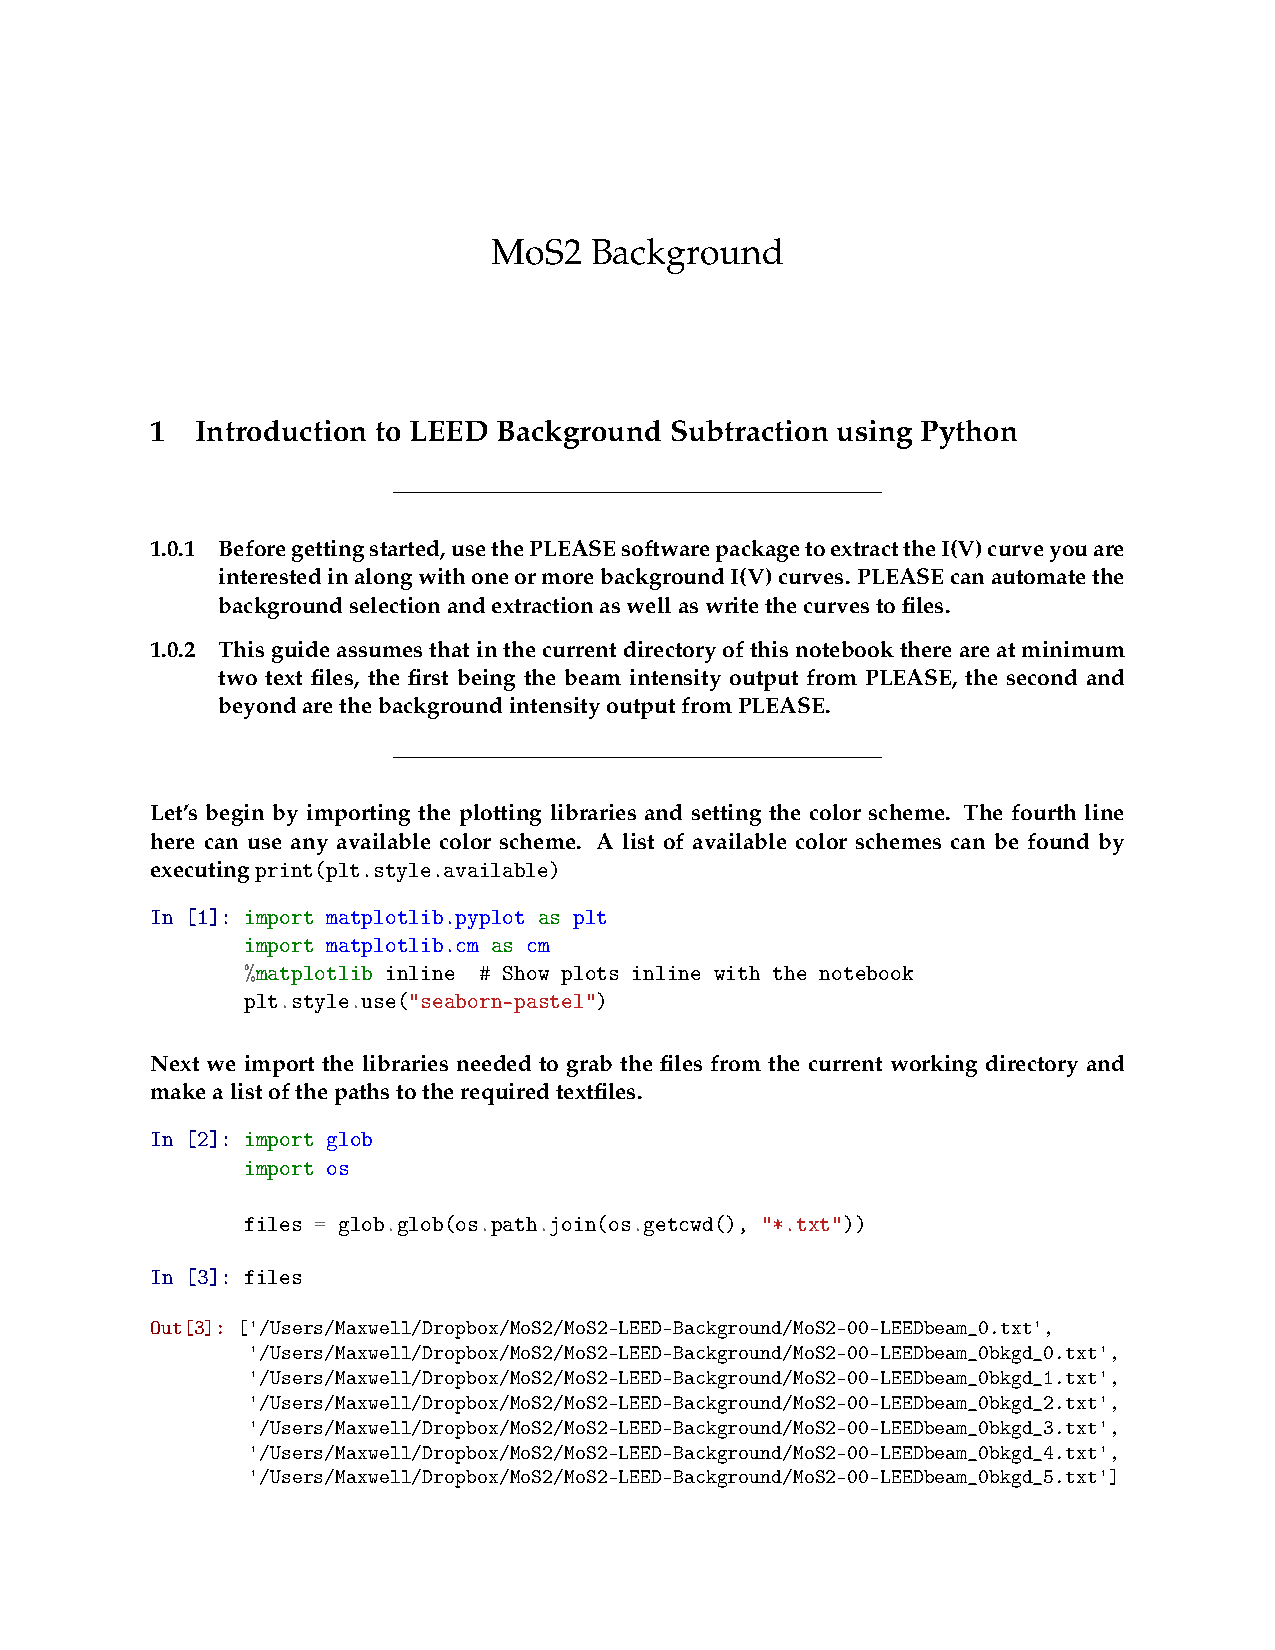
\includepdf[pages={-}, pagecommand={}]{./Appendices/MoS2-Background.pdf}
               % APPENDIX B
% \chapter{\sc Appendix C}
\label{app:Appendix-C}

% --- Insert Text --- %
\Blindtext
% ------------------- %

               % APPENDIX B
\end{appendices}
%%%%%%%%%%%%%%%%%%%%%%%%

%%%%%%%%%%%%%%%%%%%
\addcontentsline{toc}{chapter}{\sc Bibliography} % Add Bibliography into table of contents 12/05/05 Burcin Donmez
%%%%%%%%%%%%%%%%%%%%
\bibliography{./mybib}
\end{singlespace}
\end{document}

% GOOD LUCK!
